% Options for packages loaded elsewhere
\PassOptionsToPackage{unicode}{hyperref}
\PassOptionsToPackage{hyphens}{url}
%
\documentclass[
  12pt,
]{article}
\usepackage{amsmath,amssymb}
\usepackage{iftex}
\ifPDFTeX
  \usepackage[T1]{fontenc}
  \usepackage[utf8]{inputenc}
  \usepackage{textcomp} % provide euro and other symbols
\else % if luatex or xetex
  \usepackage{unicode-math} % this also loads fontspec
  \defaultfontfeatures{Scale=MatchLowercase}
  \defaultfontfeatures[\rmfamily]{Ligatures=TeX,Scale=1}
\fi
\usepackage{lmodern}
\ifPDFTeX\else
  % xetex/luatex font selection
\fi
% Use upquote if available, for straight quotes in verbatim environments
\IfFileExists{upquote.sty}{\usepackage{upquote}}{}
\IfFileExists{microtype.sty}{% use microtype if available
  \usepackage[]{microtype}
  \UseMicrotypeSet[protrusion]{basicmath} % disable protrusion for tt fonts
}{}
\makeatletter
\@ifundefined{KOMAClassName}{% if non-KOMA class
  \IfFileExists{parskip.sty}{%
    \usepackage{parskip}
  }{% else
    \setlength{\parindent}{0pt}
    \setlength{\parskip}{6pt plus 2pt minus 1pt}}
}{% if KOMA class
  \KOMAoptions{parskip=half}}
\makeatother
\usepackage{xcolor}
\usepackage[margin=1in]{geometry}
\usepackage{graphicx}
\makeatletter
\def\maxwidth{\ifdim\Gin@nat@width>\linewidth\linewidth\else\Gin@nat@width\fi}
\def\maxheight{\ifdim\Gin@nat@height>\textheight\textheight\else\Gin@nat@height\fi}
\makeatother
% Scale images if necessary, so that they will not overflow the page
% margins by default, and it is still possible to overwrite the defaults
% using explicit options in \includegraphics[width, height, ...]{}
\setkeys{Gin}{width=\maxwidth,height=\maxheight,keepaspectratio}
% Set default figure placement to htbp
\makeatletter
\def\fps@figure{htbp}
\makeatother
\setlength{\emergencystretch}{3em} % prevent overfull lines
\providecommand{\tightlist}{%
  \setlength{\itemsep}{0pt}\setlength{\parskip}{0pt}}
\setcounter{secnumdepth}{-\maxdimen} % remove section numbering
\usepackage{fontspec}
\setmainfont[
Path = C:/Users/jaketruscott/AppData/Local/Microsoft/Windows/Fonts/,
Extension = .ttf,
UprightFont = Mulish-Regular,
BoldFont = Mulish-Bold,
ItalicFont = Mulish-Italic,
BoldItalicFont = Mulish-BoldItalic
]{Mulish}

\usepackage{tikz}
\usepackage{atbegshi}
\usepackage{multicol}
\usepackage{array}
\usepackage{fontawesome5}
\usepackage{amsmath}
\usepackage{hyperref}
\usetikzlibrary{calc}
\usepackage{xcolor}
\usepackage{geometry}
\usepackage{tocloft}
\newcolumntype{L}[1]{>{\raggedright\arraybackslash}m{#1}}
\newcolumntype{C}[1]{>{\centering\arraybackslash}m{#1}}
\setlength{\cftbeforesecskip}{8pt}
\setlength{\cftbeforesubsecskip}{7pt}
\geometry{paperwidth=13.333in, paperheight=7.5in, margin=0.25in}
\setlength{\footskip}{18pt} % adjust 15–25pt depending on taste
\definecolor{dispatchBlue}{HTML}{112537}
\definecolor{dispatchRed}{HTML}{C41E3A}
\usepackage{titlesec}
\titleformat{\section} {\color{dispatchRed}\fontsize{35pt}{38pt}\selectfont\bfseries} {\thesection}{1em}{}
\titleformat{\subsection} {\color{dispatchRed}\fontsize{35pt}{38pt}\selectfont\bfseries} {\thesubsection}{1em}{}
\titleformat{\subsubsection} {\color{dispatchRed}\fontsize{35pt}{38pt}\selectfont\bfseries} {\thesubsubsection}{1em}{}
\usepackage{fancyhdr}
\fancypagestyle{fancy}{ \fancyhf{} \fancyfoot[R]{\normalsize\thepage} \renewcommand{\headrulewidth}{0pt} \renewcommand{\footrulewidth}{0pt} }
\fancypagestyle{plain}{ \fancyhf{} \fancyfoot[R]{\normalsize\thepage} \renewcommand{\headrulewidth}{0pt} \renewcommand{\footrulewidth}{0pt} }
\pagestyle{fancy}
\setlength{\footskip}{15pt}
\newcommand{\sidebox}[1]{
\hspace{-2cm}
\begin{tikzpicture}[outer sep=0pt,inner sep=0pt]
\node[
fill=dispatchBlue!8,
draw=dispatchBlue,
line width=1.2pt,
rounded corners=6pt,
inner sep=10pt,
text width=10cm,
align=left,
font=\footnotesize, 
]{
#1
};
\end{tikzpicture}
}

\newcommand{\footernote}[1]{
\begin{tikzpicture}[remember picture,overlay]

% Box dimensions
\coordinate (boxSW) at ($(current page.south west)+(0.5in,0.10in)$);
\coordinate (boxNE) at ($(current page.south east)+(-0.5in,1.15in)$);

% Draw box
\filldraw[
  fill=dispatchBlue!8,
  draw=dispatchBlue,
  line width=1.2pt,
  rounded corners=6pt
]
(boxSW) rectangle (boxNE);

% Text
\node[
anchor=center,
text width=11.5in,
align=left,
font=\footnotesize
]
at ($(boxSW)!0.5!(boxNE)$)
{#1};

\end{tikzpicture}
}

\newcommand{\footernoteopinionlengths}[1]{
\begin{tikzpicture}[remember picture,overlay]

% Box dimensions
\coordinate (boxSW) at ($(current page.south west)+(0.5in,0.10in)$);
\coordinate (boxNE) at ($(current page.south east)+(-0.5in,1.9in)$);

% Draw box
\filldraw[
  fill=dispatchBlue!8,
  draw=dispatchBlue,
  line width=1.2pt,
  rounded corners=6pt
]
(boxSW) rectangle (boxNE);

% Text
\node[
anchor=center,
text width=11.5in,
align=left,
font=\footnotesize
]
at ($(boxSW)!0.5!(boxNE)$)
{#1};

\end{tikzpicture}
}      

\newcommand{\footernotevoting}[1]{
\begin{tikzpicture}[remember picture,overlay]

% Box dimensions
\coordinate (boxSW) at ($(current page.south west)+(0.5in,0.10in)$);
\coordinate (boxNE) at ($(current page.south east)+(-0.5in,3in)$);

% Draw box
\filldraw[
  fill=dispatchBlue!8,
  draw=dispatchBlue,
  line width=1.2pt,
  rounded corners=6pt
]
(boxSW) rectangle (boxNE);

% Text
\node[
anchor=center,
text width=11.5in,
align=left,
font=\footnotesize
]
at ($(boxSW)!0.5!(boxNE)$)
{#1};

\end{tikzpicture}
}      
\usepackage{booktabs}
\usepackage{longtable}
\usepackage{array}
\usepackage{multirow}
\usepackage{wrapfig}
\usepackage{float}
\usepackage{colortbl}
\usepackage{pdflscape}
\usepackage{tabu}
\usepackage{threeparttable}
\usepackage{threeparttablex}
\usepackage[normalem]{ulem}
\usepackage{makecell}
\usepackage{xcolor}
\ifLuaTeX
  \usepackage{selnolig}  % disable illegal ligatures
\fi
\usepackage{bookmark}
\IfFileExists{xurl.sty}{\usepackage{xurl}}{} % add URL line breaks if available
\urlstyle{same}
\hypersetup{
  hidelinks,
  pdfcreator={LaTeX via pandoc}}

\author{}
\date{\vspace{-2.5em}}

\begin{document}

\begin{titlepage}
\thispagestyle{empty}
\noindent

\vspace*{0.4cm}

\hspace*{0.05\textwidth} 
% ===== LEFT COLUMN =====
\begin{minipage}[c]{0.4\textwidth}
\centering
{
\includegraphics[height=0.75\textwidth]{../images/scotusblog_logo.jpg}\par}
\vspace{2cm}
{\Huge \textbf{Final Stat Pack for the \\ 2025-26 Term}\par}
\vspace{1cm}
{\large \textbf{Updated: \today}\par}
\end{minipage}
\hfill
% ===== RIGHT COLUMN =====
\begin{minipage}[c]{0.5\textwidth}
\centering

{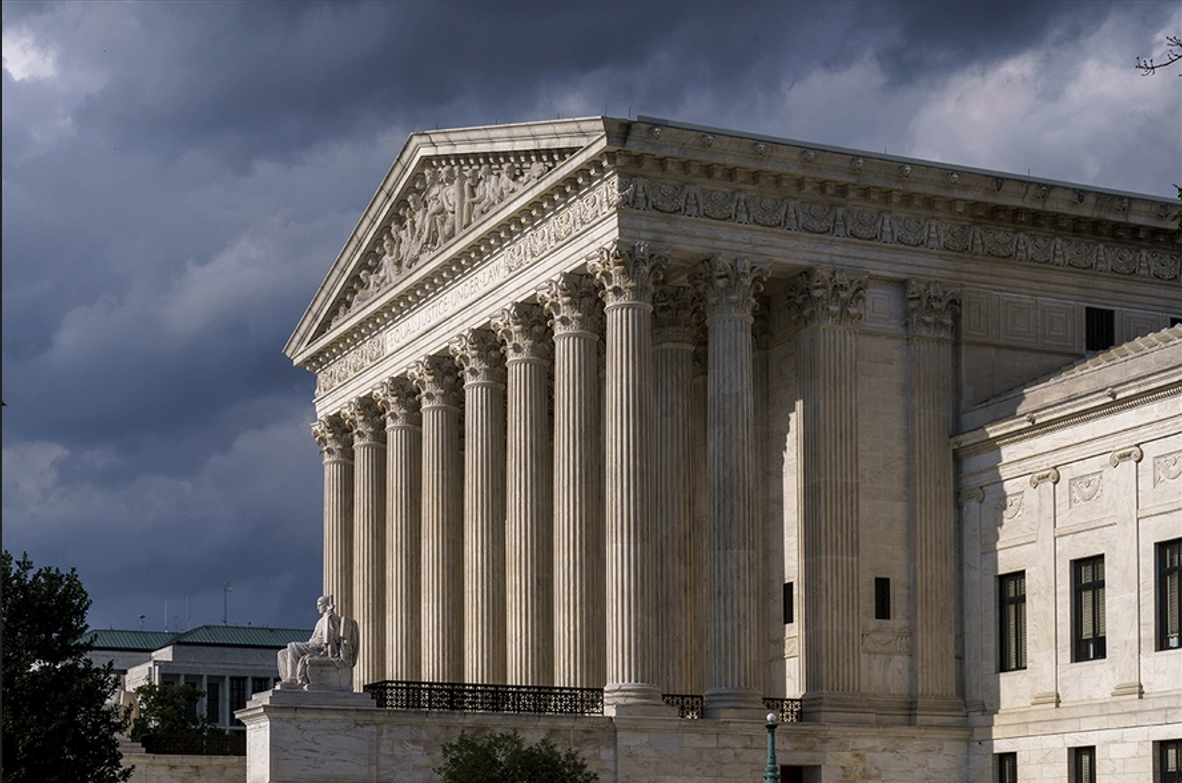
\includegraphics[height=0.6\textwidth]{../images/scotus_building.png}\par}
{\footnotesize J. Scott Applewhite/AP Photo}

\end{minipage}


\vspace*{\fill}

% AUTHOR BLOCK (flush left)
\noindent
\begin{minipage}[b]{\textwidth}
\raggedright
{\normalsize
\emph{\textbf{Compiled by Jake S. Truscott (Ph.D) and Adam Feldman (J.D., Ph.D.)}}.
}
\end{minipage}

\vspace*{1.5cm}


% ===== TIKZ FOOTER (unchanged) =====
\begin{tikzpicture}[remember picture, overlay]

\coordinate (barSW) at (current page.south west);
\coordinate (barSE) at ($(current page.south east)+(0,2.25cm)$);

\fill[dispatchBlue] (barSW) rectangle (barSE);

\coordinate (barMid) at ($(barSW)!0.5!(barSE)$);

\coordinate (colA) at ($(current page.south west)!0.125!(current page.south east)$);
\coordinate (colB) at ($(current page.south west)!0.35!(current page.south east)$);
\coordinate (colC) at ($(current page.south west)!0.525!(current page.south east)$);
\coordinate (colD) at ($(current page.south west)!0.8!(current page.south east)$);

\node[text=white, font=\Large, align=center] at (colA |- barMid)
{\href{https://www.scotusblog.com/}{\faDesktop\ www.scotusblog.com}};

\node[text=white, font=\Large, align=center] at (colB |- barMid)
{\href{https://twitter.com/SCOTUSblog}{
\includegraphics[height=14pt]{../images/x_logo.png}\ @SCOTUSblog}};

\node[text=white, font=\Large, align=center] at (colC |- barMid)
{\href{https://twitter.com/SCOTUSblog}{\faTiktok\ @scotusblog}};

\node[text=white, font=\Large, align=center] at (colD |- barMid)
{\href{mailto:scotusblog@thedispatch.com}{\faEnvelope\ scotusblog@thedispatch.com}};

\end{tikzpicture}

\end{titlepage}

\clearpage
\begingroup
\pagestyle{empty}
\pagenumbering{gobble}

\section*{Table of Contents}

\nopagebreak

\renewcommand{\contentsname}{}

\vspace{-1.25cm}

\makeatletter
\renewcommand{\@dotsep}{4.5}
\makeatother

\renewcommand{\cftsubsecfont}{\footnotesize}
\renewcommand{\cftsubsecpagefont}{\footnotesize}

\setlength{\cftbeforesubsecskip}{-1.5pt}

\tableofcontents

\clearpage
\endgroup

\pagenumbering{arabic}
\setcounter{page}{1}
\pagestyle{fancy}

\clearpage
\thispagestyle{fancy}
\pagenumbering{arabic}
\setcounter{page}{1}

\section{Introduction}

{\Large \textbf{\underline{Key Findings in the Stat Pack for the 2025-26 term}}} \par \vspace{1cm}

{\large \hspace{2.5mm} \textbf{Test 1}}. Information sample 1 \par  \vspace{1cm}

{\large \hspace{2.5mm}  \textbf{Test 2}}. Information sample 2 \par  \vspace{1cm}

{\large \hspace{2.5mm}  \textbf{Test 3}}. Information sample 3 \par  \vspace{1cm}

{\large \hspace{2.5mm}  \textbf{Test 4}}. Information sample 4 \par  \vspace{1cm}

{\large \hspace{2.5mm}  \textbf{Test 5}}. Information sample 5 \par  \vspace{1cm}

{\large \hspace{2.5mm}  \textbf{Test 6}}. Information sample 6 \par  \vspace{1cm}


\newpage

\section{Opinions Over Time}

\begin{figure}
    \centering
    
\includegraphics[width=0.65\linewidth]{../../scotusblog_replication/figures/decisions_over_time.png}
    \label{fig:opinions_over_time}
\end{figure}

\newpage

\vspace{-5mm}

\section{Makeup of the Opinions of the Court}

\begingroup\fontsize{10}{12}\selectfont

\begin{longtable}[t]{>{\raggedright\arraybackslash}p{5in}>{\centering\arraybackslash}p{3in}>{\centering\arraybackslash}p{3in}}
\toprule
\multicolumn{1}{c}{\textbf{Case Name}} & \multicolumn{1}{c}{\textbf{Abbreviation}} & \multicolumn{1}{c}{\textbf{Issue}}\\
\midrule
\endfirsthead
\multicolumn{3}{@{}l}{\textit{(continued)}}\\
\toprule
\multicolumn{1}{c}{\textbf{Case Name}} & \multicolumn{1}{c}{\textbf{Abbreviation}} & \multicolumn{1}{c}{\textbf{Issue}}\\
\midrule
\endhead

\endfoot
\bottomrule
\endlastfoot
\cellcolor{gray!10}{Abouammo v. United States} & \cellcolor{gray!10}{Abouammo} & \cellcolor{gray!10}{Criminal Procedure}\\
Barrett v. United States & Barrett & Criminal Law\\
\cellcolor{gray!10}{Berk v. Choy} & \cellcolor{gray!10}{Berk} & \cellcolor{gray!10}{Civil Procedure}\\
Blanche, Acting Atty Gen. v. Lau & Lau & Immigration\\
\cellcolor{gray!10}{Bost v. IL Bd. Of Elections} & \cellcolor{gray!10}{Bost} & \cellcolor{gray!10}{Federal Jurisdiction}\\
Bowe v. United States & Bowe & Habeas Corpus\\
\cellcolor{gray!10}{Case v. Montana} & \cellcolor{gray!10}{Case} & \cellcolor{gray!10}{Fourth Amendment}\\
Chatrie v. United States & Chatrie & Fourth Amendment\\
\cellcolor{gray!10}{Chevron USA Inc. v. Plaquemines Parish} & \cellcolor{gray!10}{Plaquemines Parish} & \cellcolor{gray!10}{Federal Jurisdiction}\\
Chiles v. Salazar & Chiles & Free Speech\\
\cellcolor{gray!10}{Cisco Systems, Inc. v. DOE I} & \cellcolor{gray!10}{Cisco} & \cellcolor{gray!10}{Human Rights Litigation}\\
Clark v. Sweeney & Clark & Appellate Procedure\\
\cellcolor{gray!10}{Coney Island Auto Parts, Inc. v. Burton} & \cellcolor{gray!10}{Coney Island Auto} & \cellcolor{gray!10}{Civil Procedure}\\
Cox Communications v. Sony Music Entertainment & Cox & Copyright\\
\cellcolor{gray!10}{District of Columbia v. R.W.} & \cellcolor{gray!10}{R.W.} & \cellcolor{gray!10}{Fourth Amendment}\\
Doe v. Dynamic Physical Therapy, LLC & Dynamic PT & Federal Supremacy\\
\cellcolor{gray!10}{Ellingburg v. United States} & \cellcolor{gray!10}{Ellingburg} & \cellcolor{gray!10}{Criminal Sentencing}\\
Enbridge Energy, LP v. Nessel & Enbridge & Federal Jurisdiction\\
\cellcolor{gray!10}{Exxon Mobil Corp. v. Corporacion Cimex, S.A.} & \cellcolor{gray!10}{Exxon} & \cellcolor{gray!10}{Foreign Sovereign Immunity}\\
FCC v. AT\&T & AT\&T & Administrative Law\\
\cellcolor{gray!10}{FS Credit Opportunities Corp. v. Saba Capital Master Fund} & \cellcolor{gray!10}{FS Credit} & \cellcolor{gray!10}{Securities Law}\\
Fernandez v. United States & Fernandez & Habeas Corpus\\
\cellcolor{gray!10}{First Choice Women's Resource Centers v. Davenport} & \cellcolor{gray!10}{First Choice} & \cellcolor{gray!10}{Freedom of Association}\\
Flowers Foods, Inc. v. Brock & Flowers Foods & Arbitration\\
\cellcolor{gray!10}{GEO Group, Inc. v. Menocal} & \cellcolor{gray!10}{GEO Group} & \cellcolor{gray!10}{Federal Jurisdiction}\\
Galette v. NJ Transit Corp. & Galette & Sovereign Immunity\\
\cellcolor{gray!10}{Hain Celestial Group v. Palmquist} & \cellcolor{gray!10}{Hain Celestial Grp.} & \cellcolor{gray!10}{Federal Jurisdiction}\\
Hamm v. Smith & Hamm & Death Penalty\\
\cellcolor{gray!10}{Havana Docks Corp. v. Royal Caribbean  Cruises} & \cellcolor{gray!10}{Havana Docks} & \cellcolor{gray!10}{Foreign Affairs}\\
Hencely v. Fluor Corp & Hencely & Federal Preemption\\
\cellcolor{gray!10}{Hikma Pharmaceuticals USA Inc. v. Amarin Pharma, Inc.} & \cellcolor{gray!10}{Hikma} & \cellcolor{gray!10}{Patent Law}\\
Hunter v. United States & Hunter & Criminal Procedure\\
\cellcolor{gray!10}{Jules v. Andre Balazs Properties} & \cellcolor{gray!10}{Jules} & \cellcolor{gray!10}{Arbitration}\\
Keathley v. Buddy Ayers Construction, Inc. & Keathley & Bankruptcy\\
\cellcolor{gray!10}{Klein v. Martin} & \cellcolor{gray!10}{Klein} & \cellcolor{gray!10}{Habeas Corpus}\\
Landor v. LA DOC & Landor & Religious Liberty\\
\cellcolor{gray!10}{Learning Resources, Inc. v. Trump, President of U.S.} & \cellcolor{gray!10}{Learning Resources} & \cellcolor{gray!10}{Presidential Power}\\
Little v. Hecox & Little & Gender Identity\\
\cellcolor{gray!10}{Louisiana v. Callais} & \cellcolor{gray!10}{Callais} & \cellcolor{gray!10}{Redistricting}\\
M \& K Employee Solutions v. Trustees of the IAM Pension Fund & IAM Pension Fund & ERISA\\
\cellcolor{gray!10}{Margolin v. NAIJ} & \cellcolor{gray!10}{Margolin} & \cellcolor{gray!10}{Appellate Procedure}\\
McCarthy v. Hernandez & McCarthy & Habeas Corpus\\
\cellcolor{gray!10}{Monsanto Co. v. Durnell} & \cellcolor{gray!10}{Monsanto} & \cellcolor{gray!10}{Federal Preemption}\\
Montgomery v. Caribe Transport II, LLC & Montgomery & Federal Preemption\\
\cellcolor{gray!10}{Mullin, Sec. of Homeland Security v. Doe} & \cellcolor{gray!10}{Mullin v. Doe} & \cellcolor{gray!10}{Immigration}\\
Mullin, Sec. of Homeland v. Al Otro Lado & Al Otro Lado & Immigration\\
\cellcolor{gray!10}{NRSC v. FEC} & \cellcolor{gray!10}{NRSC} & \cellcolor{gray!10}{Campaign Finance}\\
Olivier v. City of Brandon & Olivier & Civil Rights\\
\cellcolor{gray!10}{Pitchford v. Cain} & \cellcolor{gray!10}{Pitchford} & \cellcolor{gray!10}{Habeas Corpus}\\
Pitts v. Mississippi & Pitts & Confrontation Clause\\
\cellcolor{gray!10}{Pung v. Isabella County} & \cellcolor{gray!10}{Pung} & \cellcolor{gray!10}{Property Rights}\\
Rico v. United States & Rico & Criminal Sentencing\\
\cellcolor{gray!10}{Rutherford v. United States} & \cellcolor{gray!10}{Rutherford} & \cellcolor{gray!10}{Criminal Sentencing}\\
Sripetch v. SEC & Sripetch & Securities Law\\
\cellcolor{gray!10}{T. M. v. Univ. of MD Medical Sys. Corp.} & \cellcolor{gray!10}{UMD Medical} & \cellcolor{gray!10}{Federal Jurisdiction}\\
Trump v. Barbara & Barbara & Citizenship\\
\cellcolor{gray!10}{Trump, President of U.S. v. Cook} & \cellcolor{gray!10}{Cook} & \cellcolor{gray!10}{Presidential Power}\\
Trump, President of United States v. Slaughter & Slaughter & Presidential Power\\
\cellcolor{gray!10}{USPS v. Konan} & \cellcolor{gray!10}{USPS} & \cellcolor{gray!10}{Federal Tort Claims}\\
United States v. Hemani & Hemani & Criminal Law\\
\cellcolor{gray!10}{Urias-Orellana v. Bondi, Att'y Gen.} & \cellcolor{gray!10}{Urias-Orellana} & \cellcolor{gray!10}{Immigration}\\
Villarreal v. Texas & Villarreal & Criminal Procedure\\
\cellcolor{gray!10}{Watson v. RNC} & \cellcolor{gray!10}{Watson} & \cellcolor{gray!10}{Election Law}\\
West Virginia v. B.P.J. & B.P.J. & Gender Identity\\
\cellcolor{gray!10}{Whitton v. Dixon} & \cellcolor{gray!10}{Whitton} & \cellcolor{gray!10}{Habeas Corpus}\\
Wolford v. Lopez & Wolford & Second Amendment\\
\cellcolor{gray!10}{Zorn v. Linton} & \cellcolor{gray!10}{Zorn} & \cellcolor{gray!10}{Qualified Immunity}\\*
\end{longtable}
\endgroup{}
\newpage

\section*{Most Frequent Issues}
\addcontentsline{toc}{subsection}{Most Frequent Issues}

\begin{center}
{
\renewcommand{\arraystretch}{3.5}
\begin{table}[!h]
\centering\begingroup\fontsize{11}{13}\selectfont

\begin{tabular}[t]{L{20cm}C{4cm}}
\toprule
\multicolumn{1}{c}{\textbf{Issue(s)}} & \multicolumn{1}{c}{\textbf{OT25-26 Cases}}\\
\midrule
Federal Jurisdiction, Habeas Corpus & 6\\
\cellcolor[HTML]{F5F5F5}{Immigration} & \cellcolor[HTML]{F5F5F5}{4}\\
Criminal Procedure, Criminal Sentencing, Federal Preemption, Fourth Amendment, Presidential Power & 3\\
\cellcolor[HTML]{F5F5F5}{Appellate Procedure, Arbitration, Civil Procedure, Criminal Law, Gender Identity, Securities Law} & \cellcolor[HTML]{F5F5F5}{2}\\
Administrative Law, Bankruptcy, Campaign Finance, Citizenship, Civil Rights, Confrontation Clause, Copyright, Death Penalty, Election Law, ERISA, Federal Supremacy, Federal Tort Claims, Foreign Affairs, Foreign Sovereign Immunity, Free Speech, Freedom of Association, Human Rights Litigation, Patent Law, Property Rights, Qualified Immunity, Redistricting, Religious Liberty, Second Amendment, Sovereign Immunity & 1\\
\bottomrule
\end{tabular}
\endgroup{}
\end{table}}
\end{center}

\newpage
\newpage

\section{Unanimity}

\begin{figure}
    \centering
    
\includegraphics[width=0.65\linewidth]{../../scotusblog_replication/figures/unanimity_over_time.png}
    \label{fig:unanimity}
\end{figure}

\footernote{
\textbf{Description}: This figure shows the percentage of unanimous decisions (i.e., cases decided without any
full dissents) between OT05-OT25. These include decisions reached per curiam without any
noted dissents. Dashed red line represent longitudinal average.
}
\newpage

\addcontentsline{toc}{section}{Frequency in the Majority}
\section*{Frequency in the Majority -- All Cases}
\addcontentsline{toc}{subsection}{All Cases}
\begin{figure}
    \centering
    
\includegraphics[width=0.65\linewidth]{../../scotusblog_replication/figures/percent_in_majority.png}
    \label{fig:frequency_majority_all}
\end{figure}

\footernote{
\textbf{Description}: Figure shows the percentage of cases where each justice was in the majority coalition among all cases that they participated in (including those decided \emph{unanimously}, \emph{per curiam}, or \emph{dismissed as improvidently granted}). 
}
\newpage


\section*{Frequency in the Majority -- Non-Unanimous Cases}
\addcontentsline{toc}{subsection}{Non-Unanimous Cases}
\begin{figure}
    \centering
    
\includegraphics[width=0.65\linewidth]{../../scotusblog_replication/figures/percent_in_majority_non_unanimous_cases.png}
    \label{fig:frequency_majority_non_unanimous}
\end{figure}

\footernote{
\textbf{Description}: Figure shows the percentage of cases where each justice was in the majority coalition among cases decided without a unanimous majority. 
}
\newpage

\section*{Frequency in the Majority -- Closely Divided Cases}
\addcontentsline{toc}{subsection}{Closely Divided Cases}
\begin{figure}
    \centering
    
\includegraphics[width=0.65\linewidth]{../../scotusblog_replication/figures/percent_in_majority_close_cases.png}
    \label{fig:frequency_majority_close_cases}
\end{figure}

\footernote{
\textbf{Description}: Figures show the percentage of cases where each justice was in the majority coalition among cases decided by (5-4) or (6-3) coalitions. 
}
\newpage

\addcontentsline{toc}{section}{Justice Agreement}
\section*{Justice Agreement -- All Cases}
\addcontentsline{toc}{subsection}{All Cases}
\noindent
\begin{tabular}{@{}m{0.68\textwidth} m{0.30\textwidth}@{}}

\includegraphics[
width=0.8\linewidth,
keepaspectratio
]{../../scotusblog_replication/figures/agreement_matrix_all_cases.png}
&
\sidebox{
\textbf{Description}: Figure shows the relative agreement (percent) in voting alignment shared between justices in all cases where justices participated during the 2025-26 term.

}

\end{tabular}
\clearpage

\section*{Justice Agreement -- Closely Divided Cases}
\addcontentsline{toc}{subsection}{Closely Divided Cases}
\noindent
\begin{tabular}{@{}m{0.68\textwidth} m{0.30\textwidth}@{}}

\includegraphics[
width=0.8\linewidth,
keepaspectratio
]{../../scotusblog_replication/figures/agreement_matrix_close_cases.png}
&
\sidebox{
\textbf{Description}: Figure shows the relative agreement (percent) in voting alignment shared between justices in cases decided by (5-4) or (6-3) coalitions in the 2025-26 term.
}

\end{tabular}
\clearpage

\addcontentsline{toc}{section}{Decisions by Vote Split}
\section*{Decisions by Vote Split -- All Cases}
\addcontentsline{toc}{subsection}{All Cases}
\begin{figure}[h!]
    \centering
    \begin{minipage}{0.32\linewidth}
        \centering
        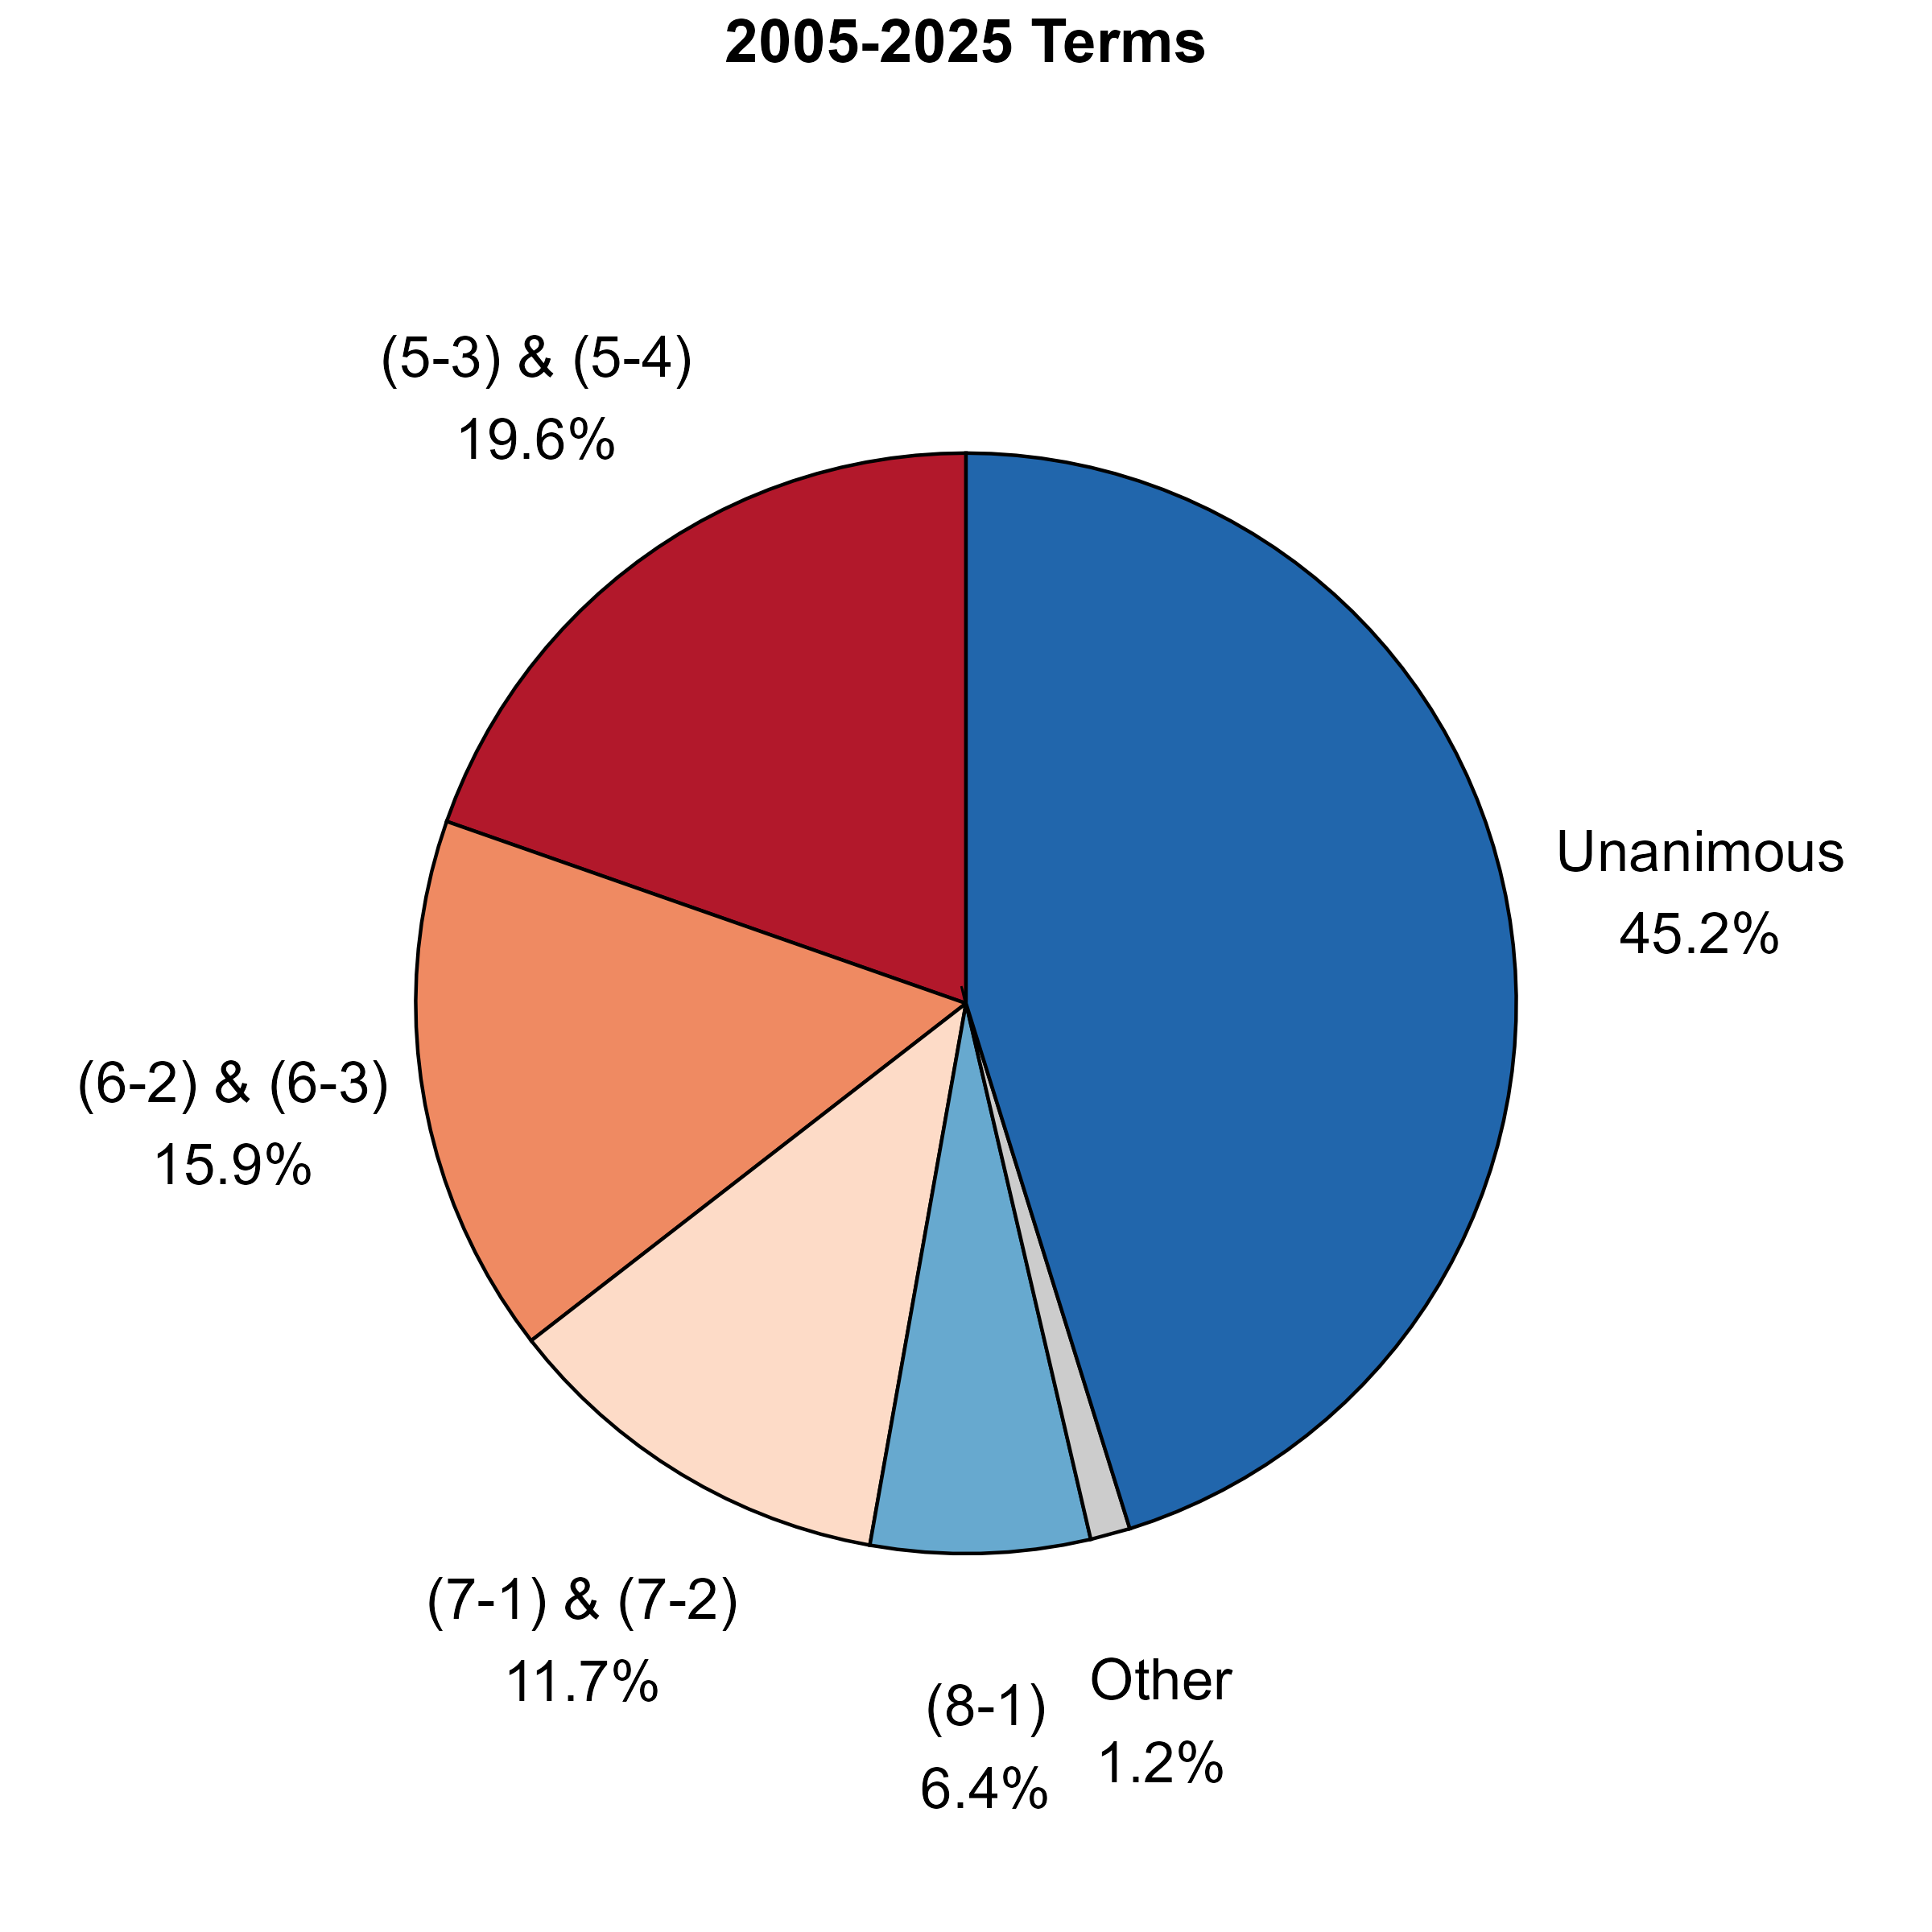
\includegraphics[width=\linewidth]{../../scotusblog_replication/figures/ot05_ot25_splits.png}
    \end{minipage}
    \hfill
    \begin{minipage}{0.32\linewidth}
        \centering
        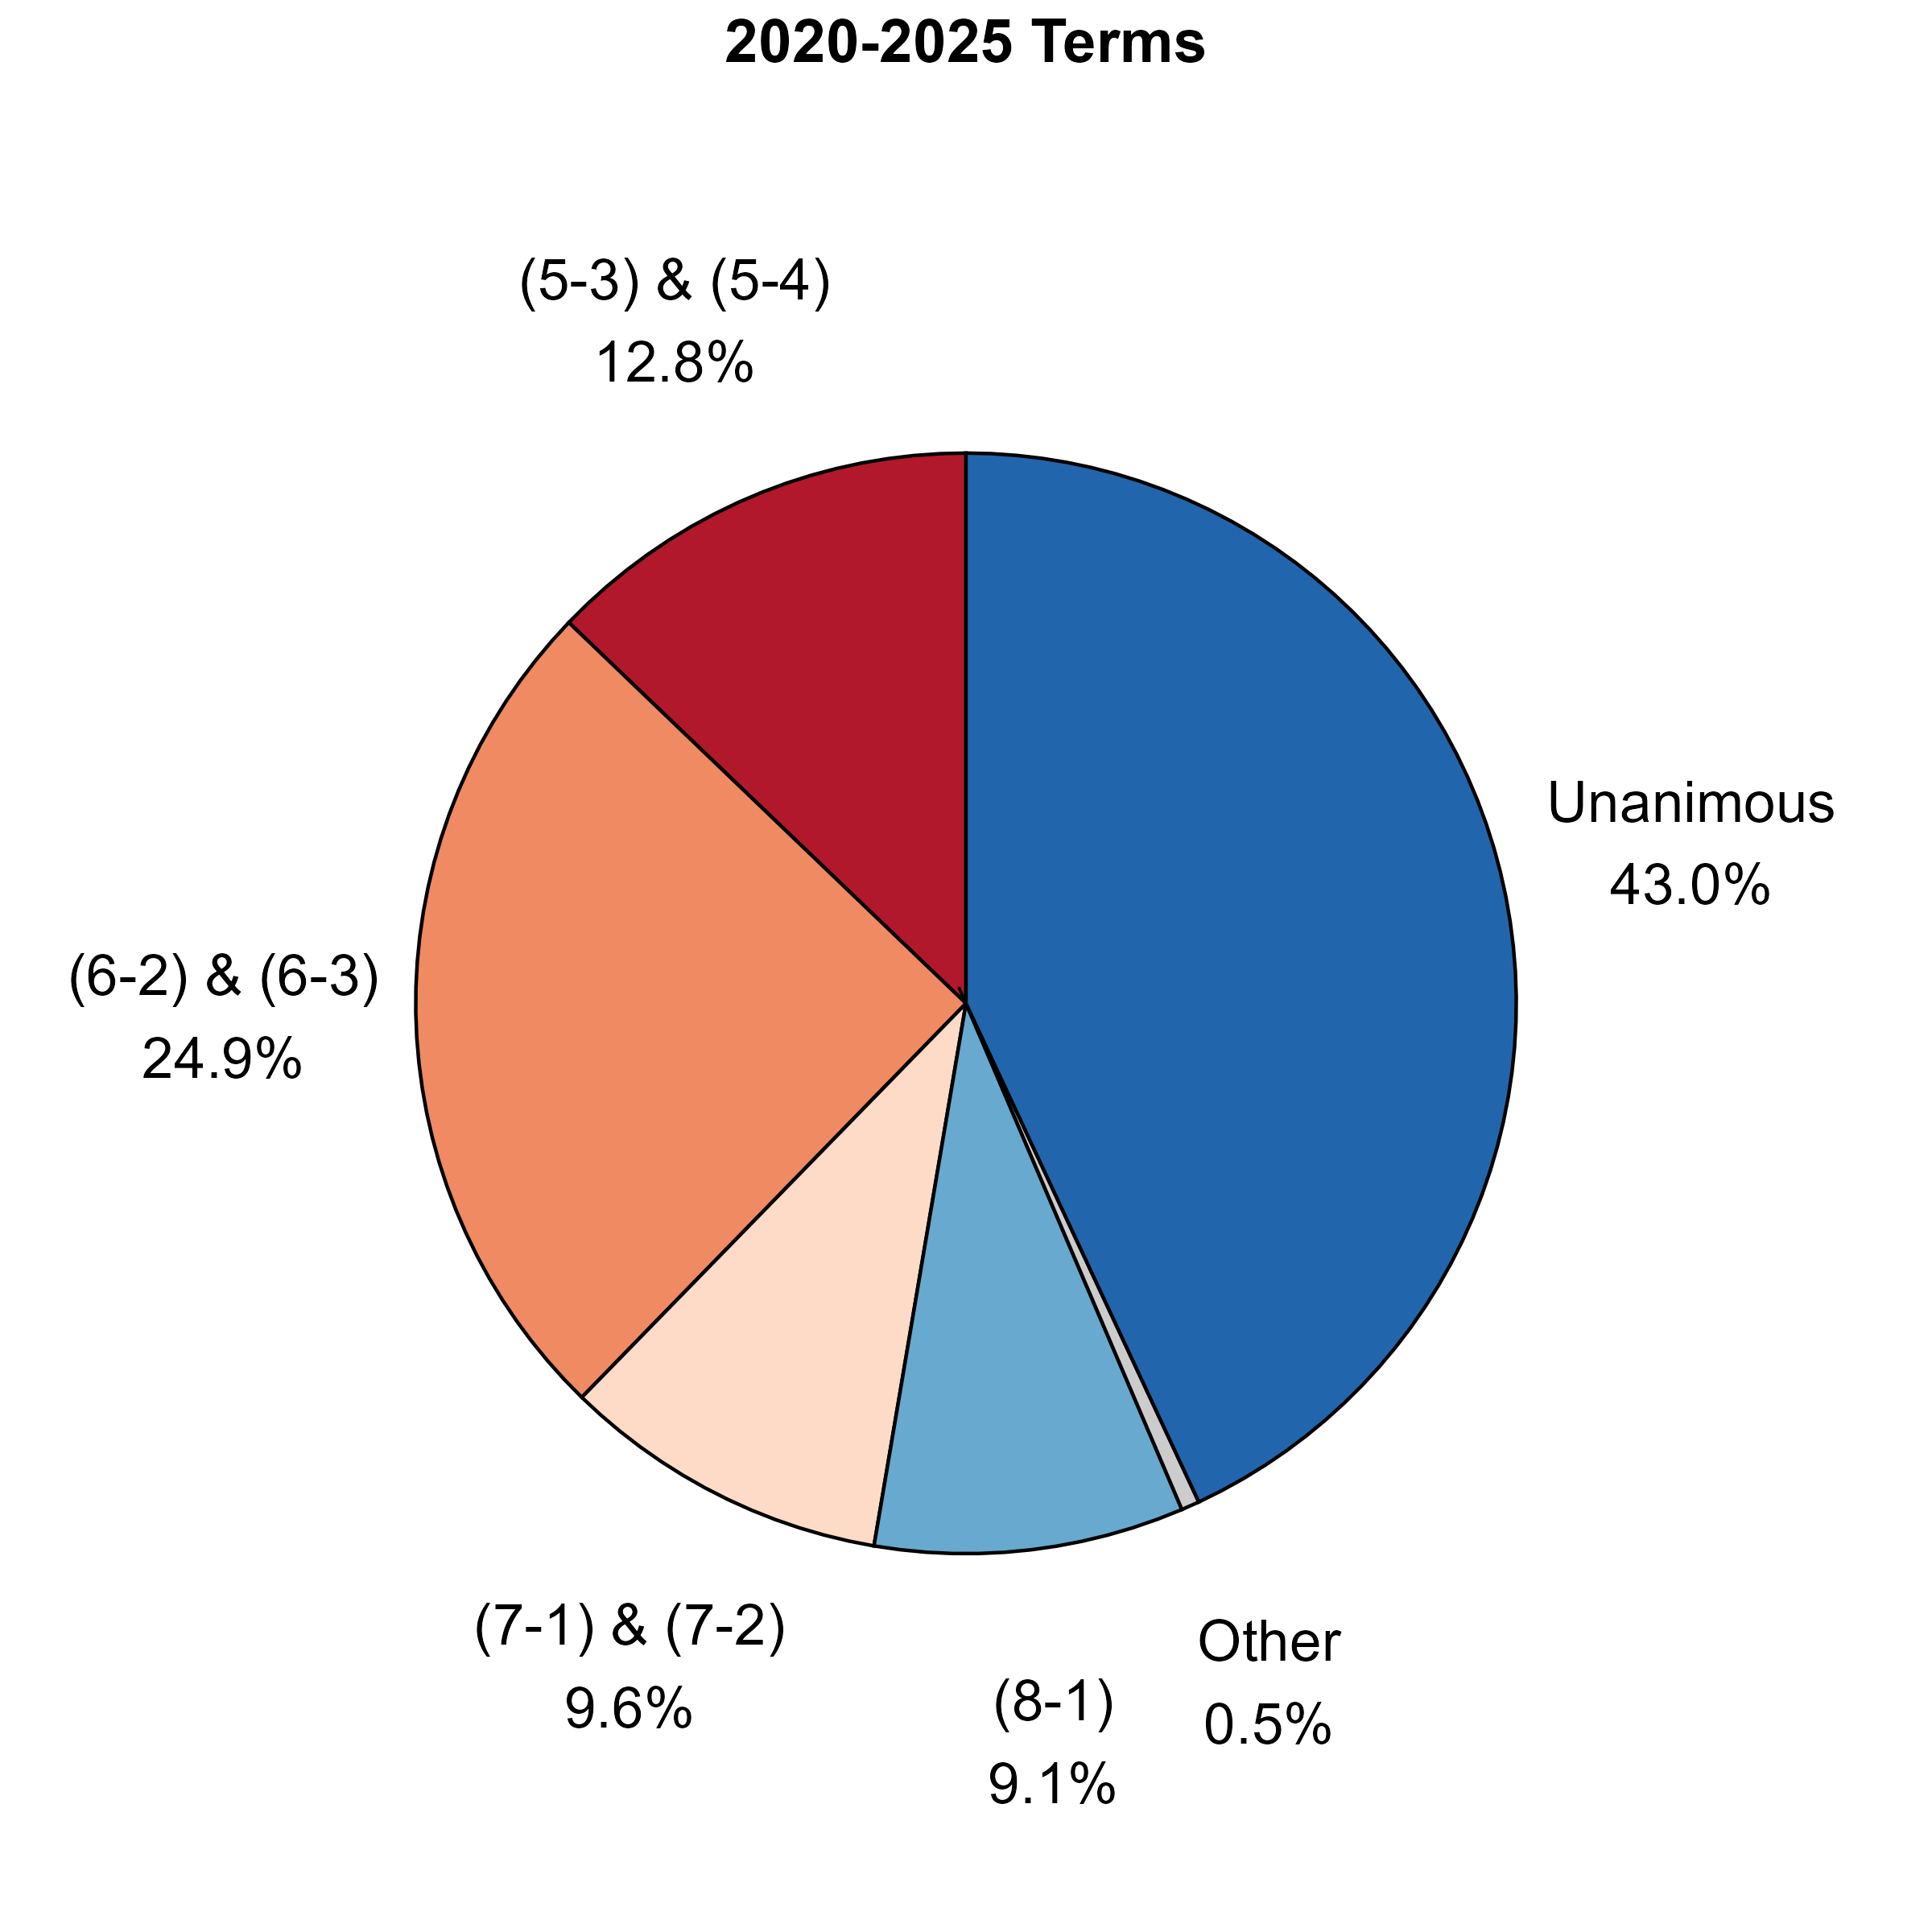
\includegraphics[width=\linewidth]{../../scotusblog_replication/figures/ot20_ot25_splits.png}
    \end{minipage}
    \hfill
    \begin{minipage}{0.32\linewidth}
        \centering
        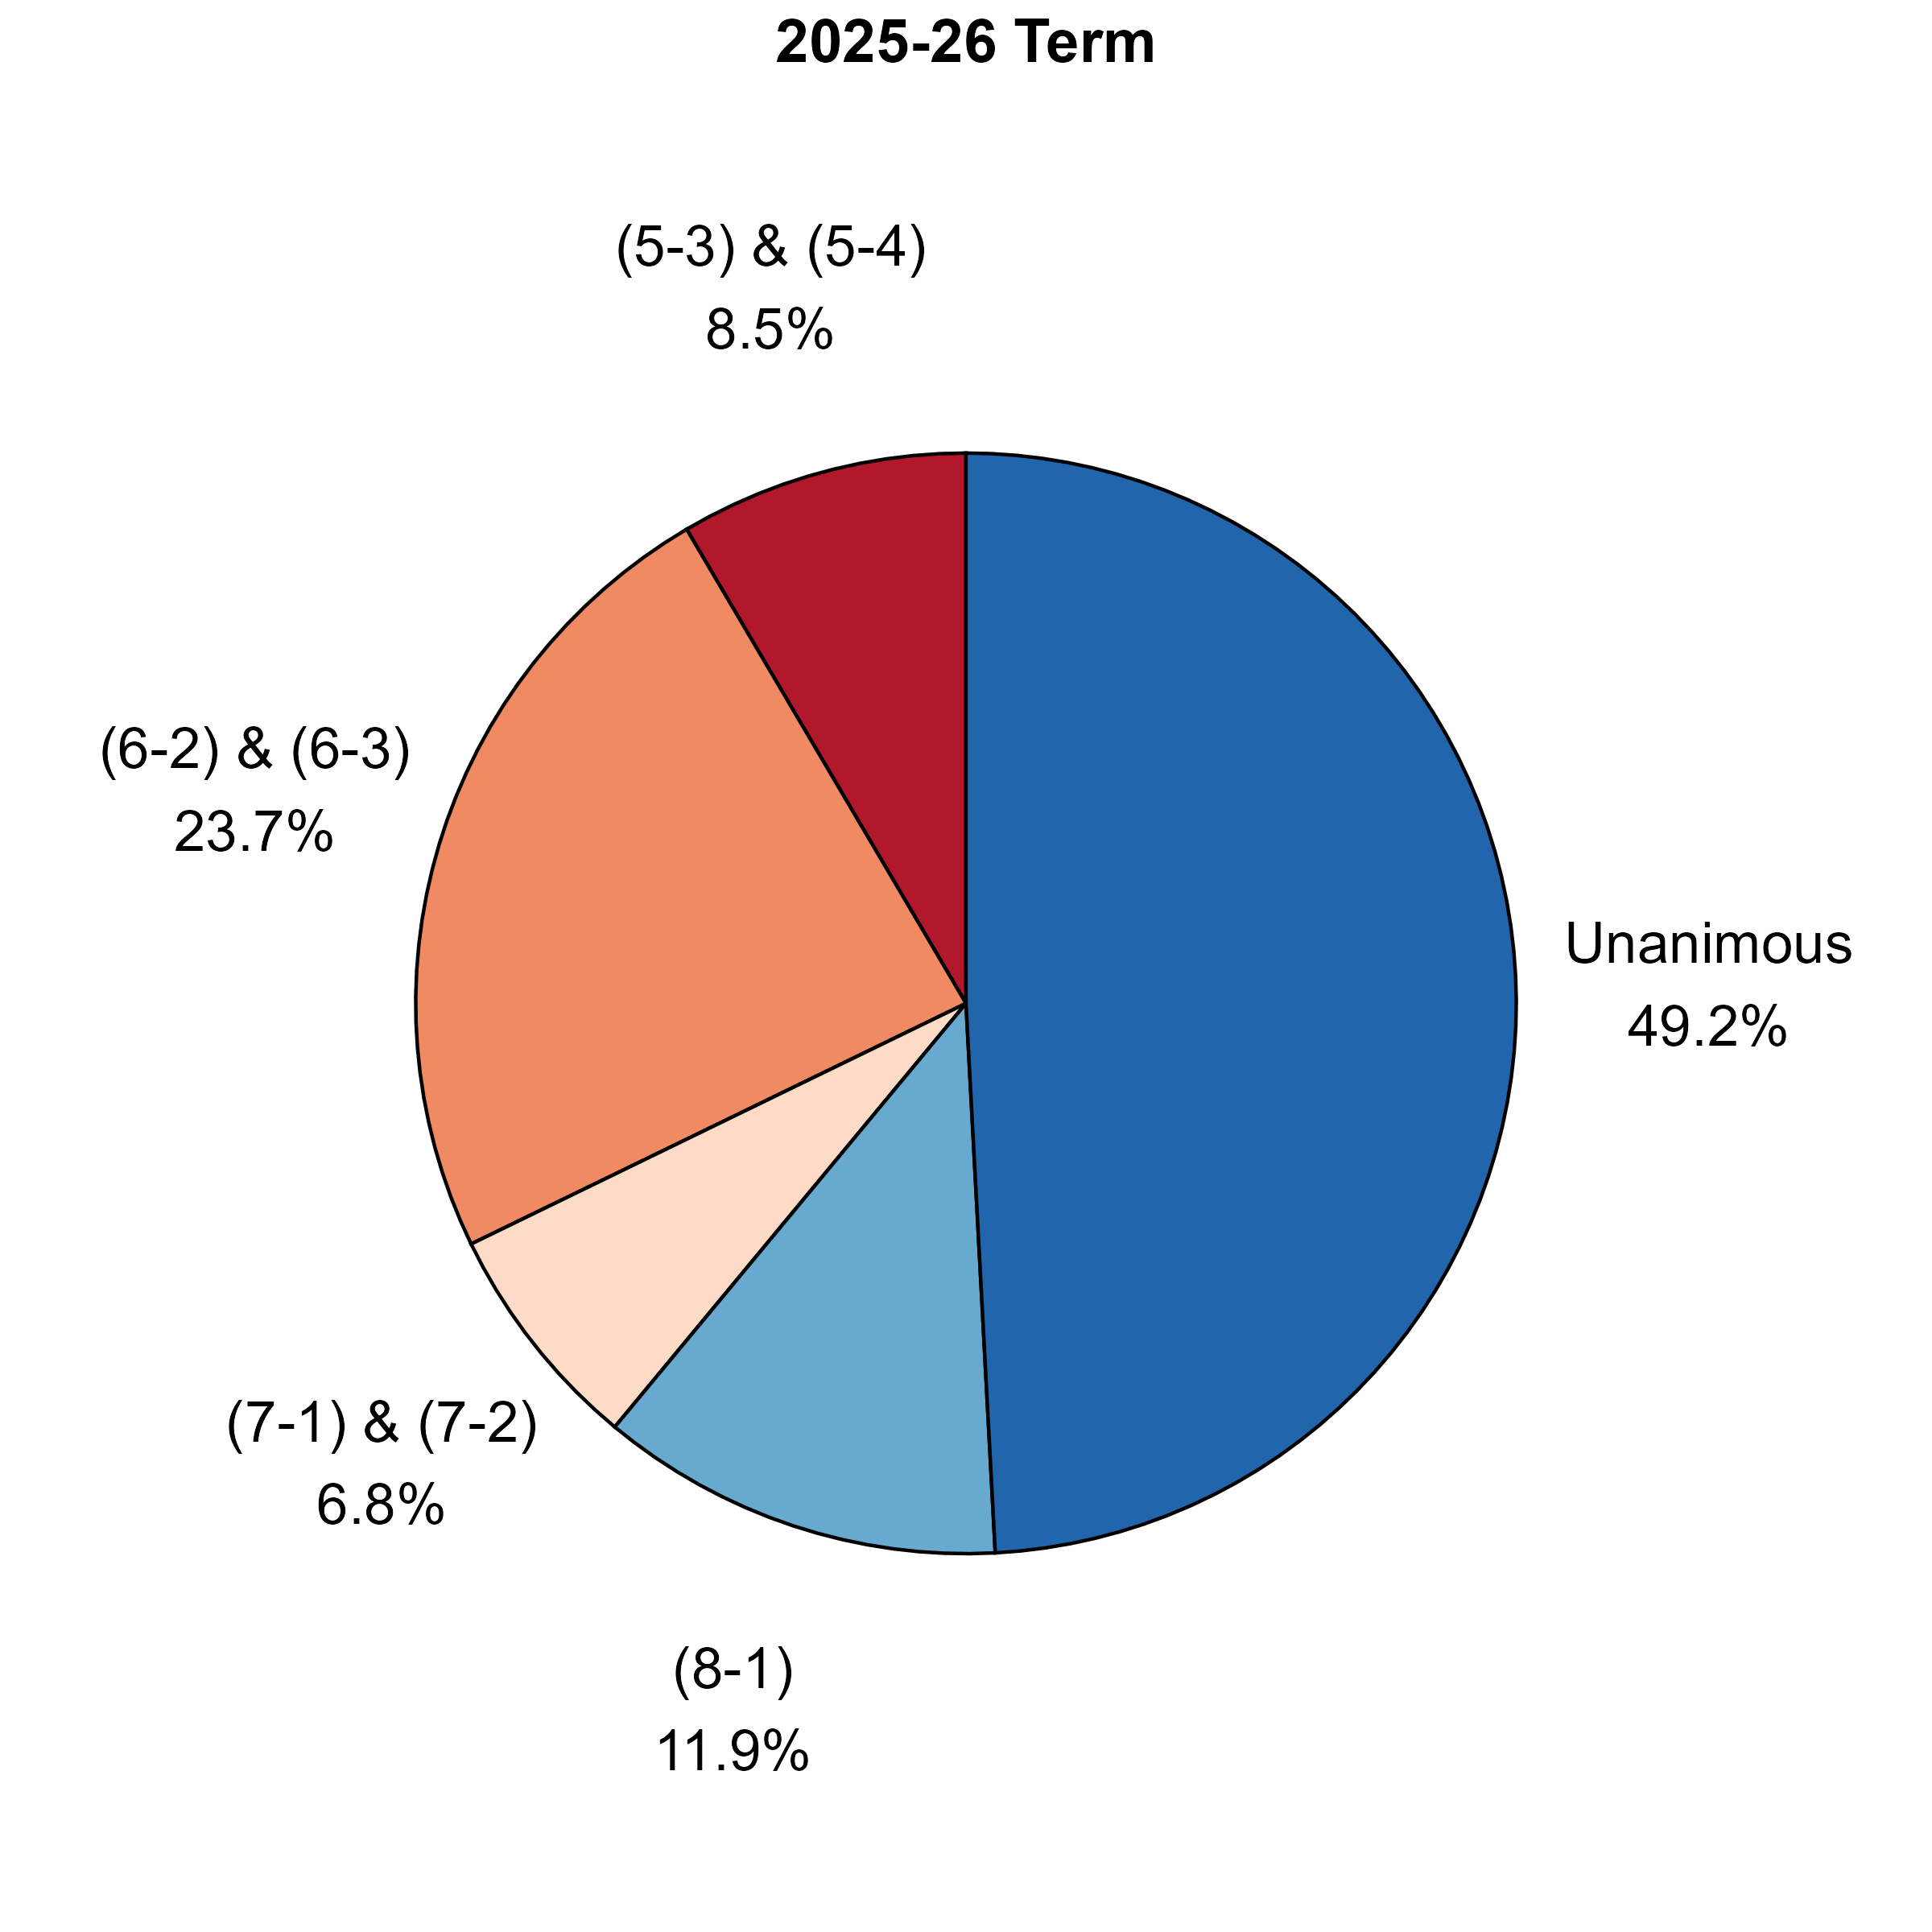
\includegraphics[width=\linewidth]{../../scotusblog_replication/figures/ot25_splits.png}
    \end{minipage}
\end{figure}

\footernote{
\textbf{Description}: Figures show the percent of cases decided by different coalition sizes between the 2005 and 2025 terms. For instances where justices were recused or did not participate in an otherwise unanimous decision, we coded these as \emph{unanimous} (e.g., 8-0 decisions were included in calculating 9-0 coalitions). 
}
\newpage



\section*{Decisions by Vote Split -- Ideologically Split Cases}
\addcontentsline{toc}{subsection}{Ideologically Split Cases}
\begin{figure}[h!]
    \centering
    \begin{minipage}{0.32\linewidth}
        \centering
        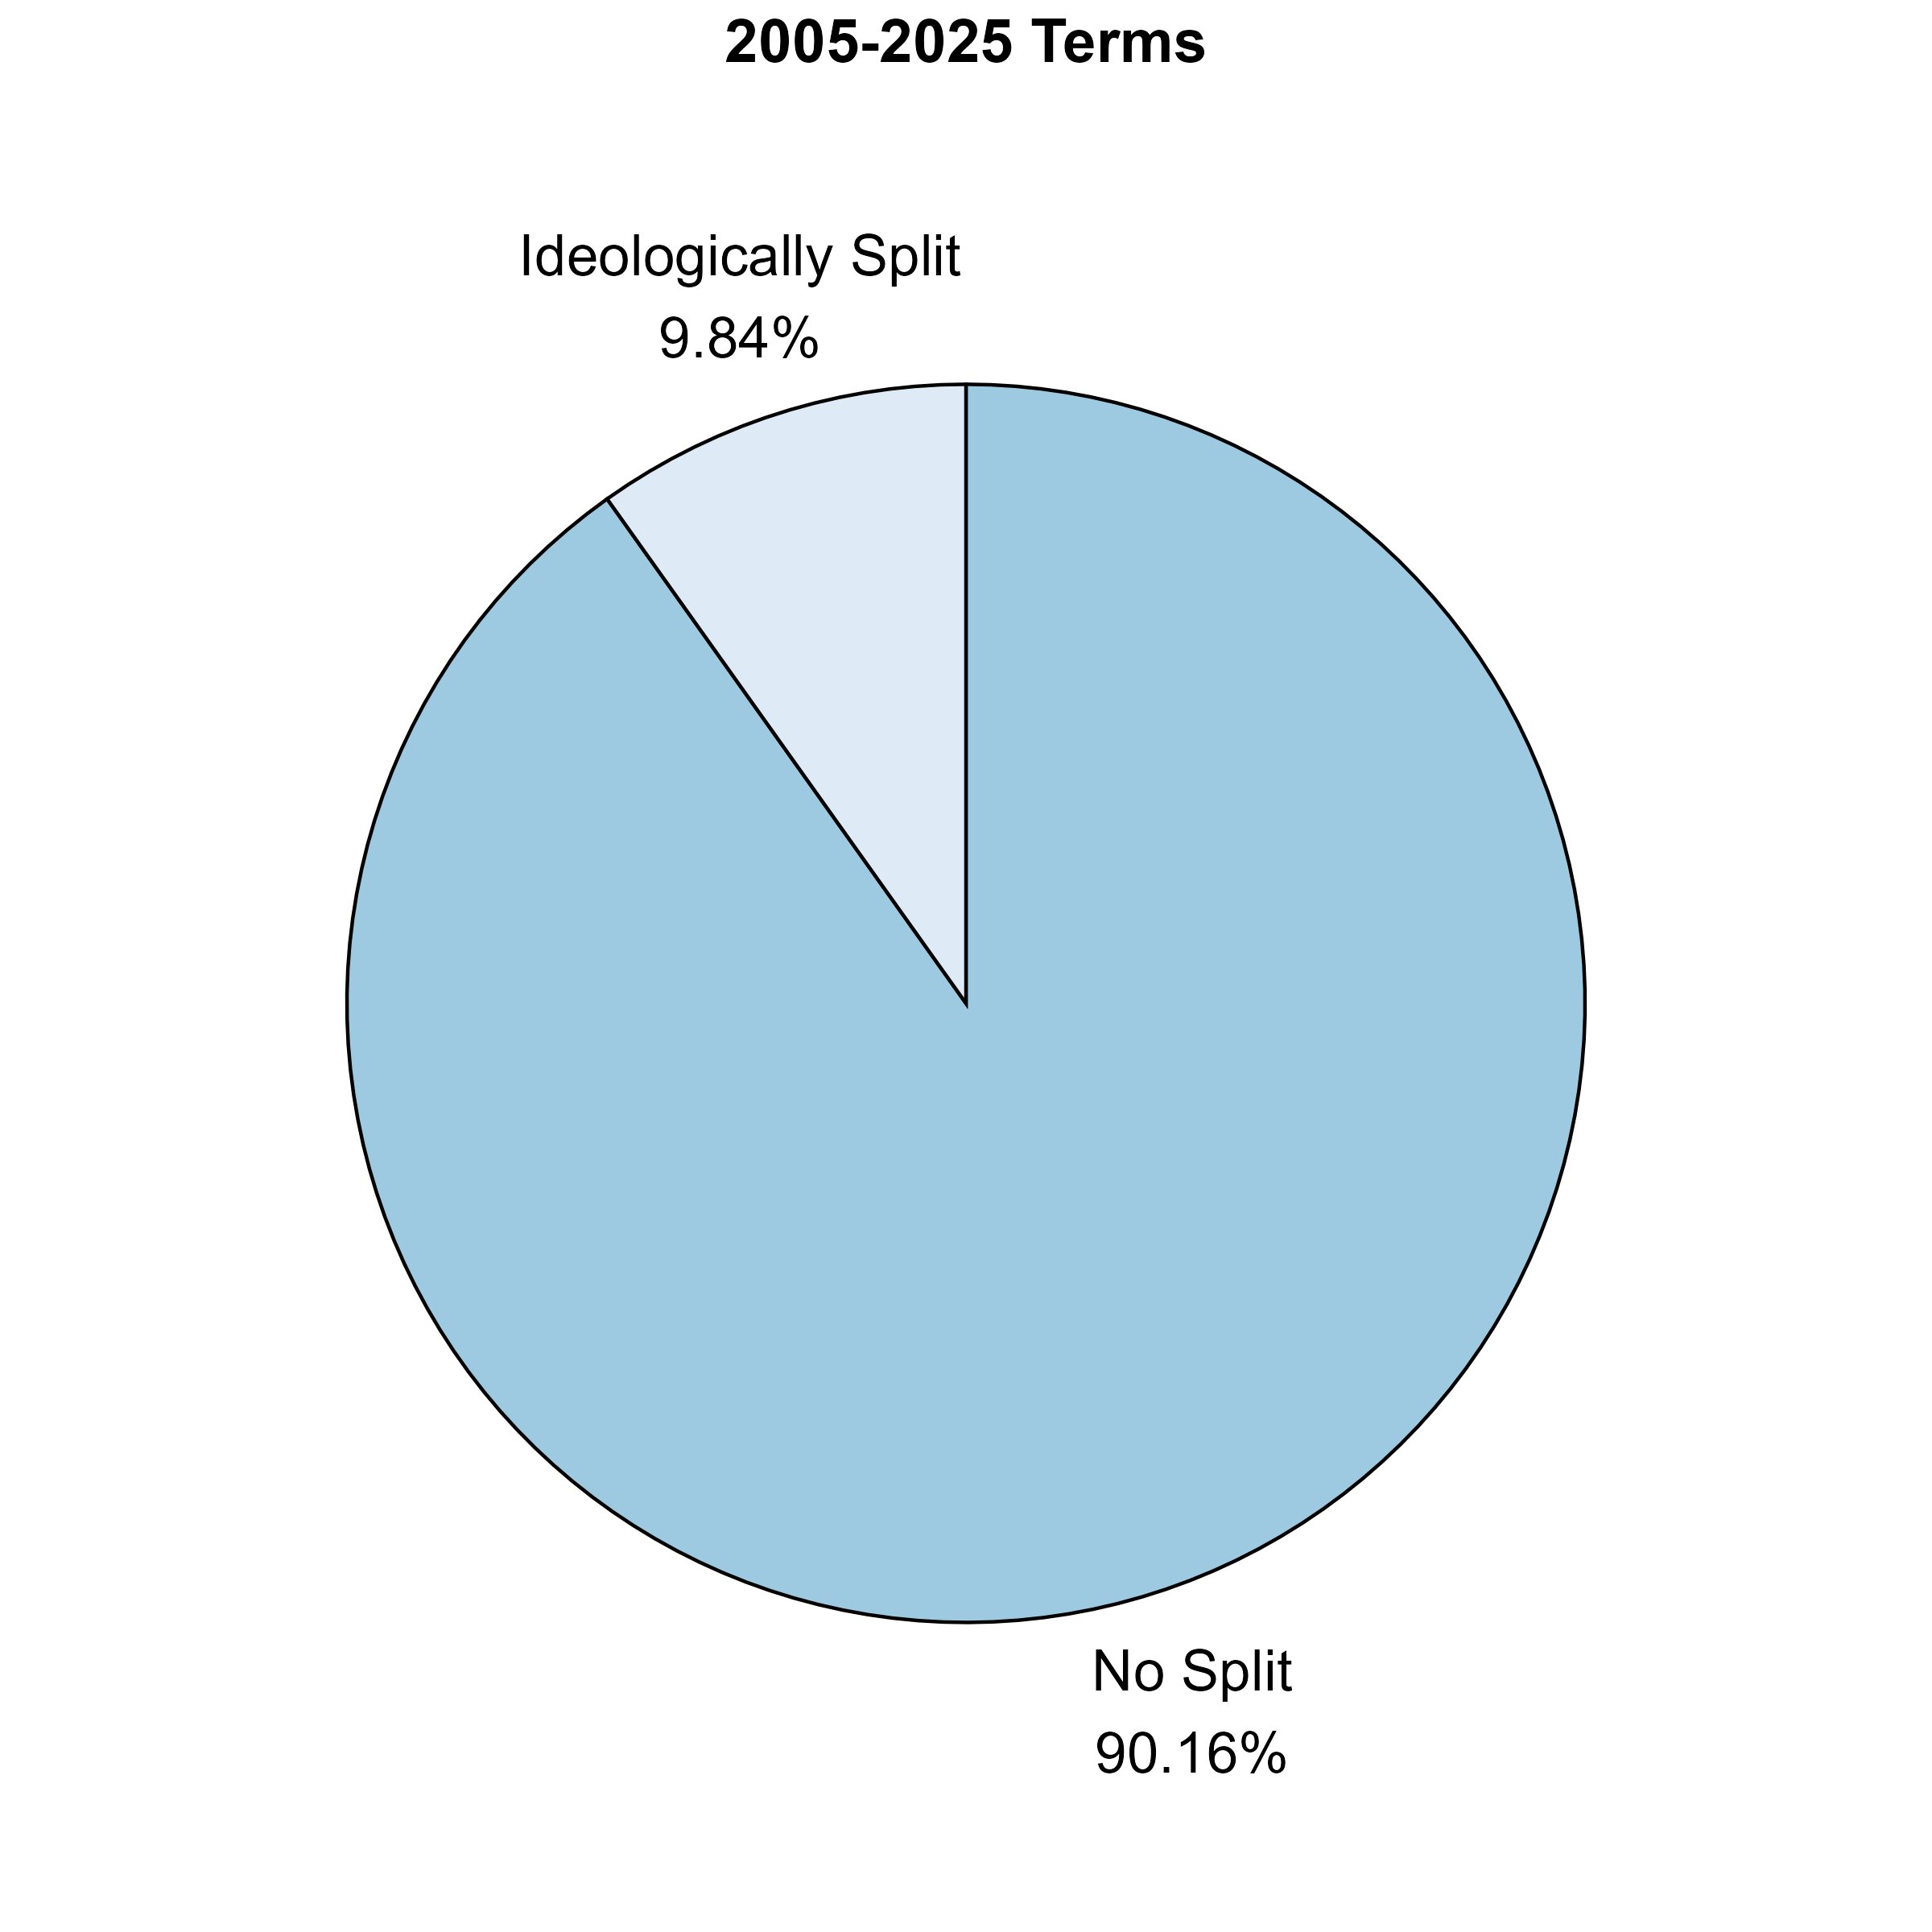
\includegraphics[width=\linewidth]{../../scotusblog_replication/figures/ot05_ot25_ideological.png}
    \end{minipage}
    \hfill
    \begin{minipage}{0.32\linewidth}
        \centering
        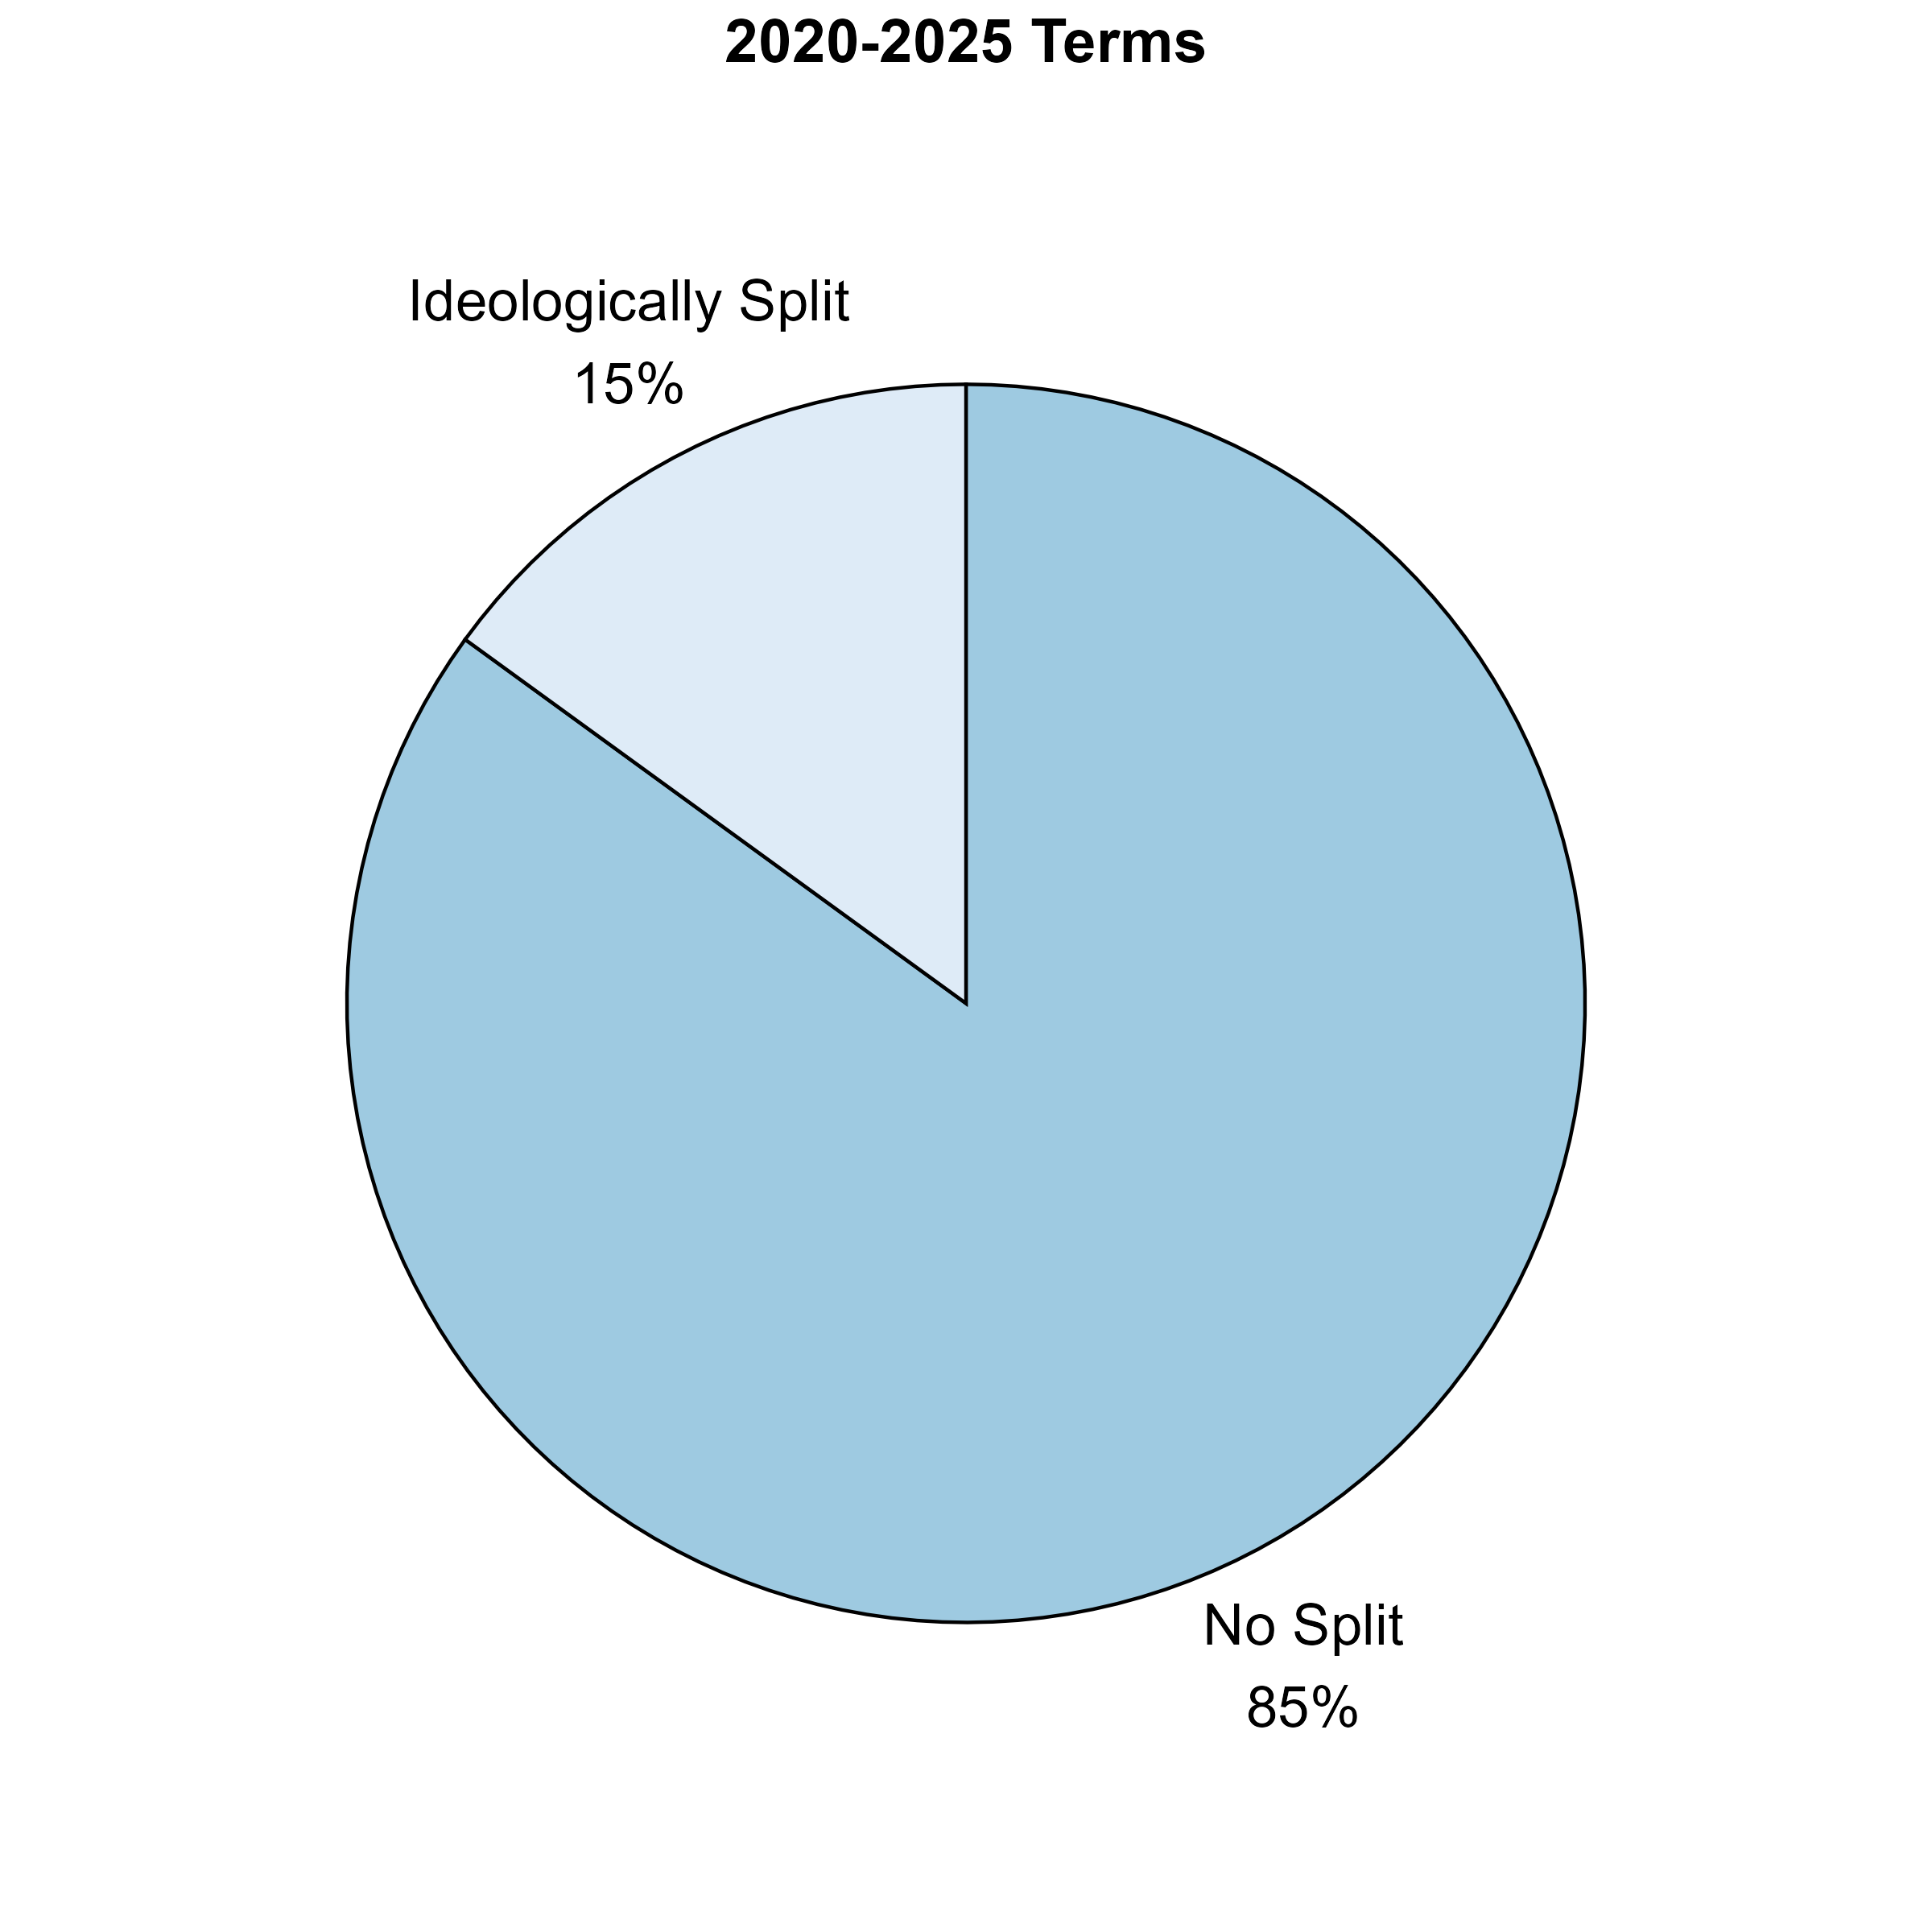
\includegraphics[width=\linewidth]{../../scotusblog_replication/figures/ot20_ot25_ideological.png}
    \end{minipage}
    \hfill
    \begin{minipage}{0.32\linewidth}
        \centering
        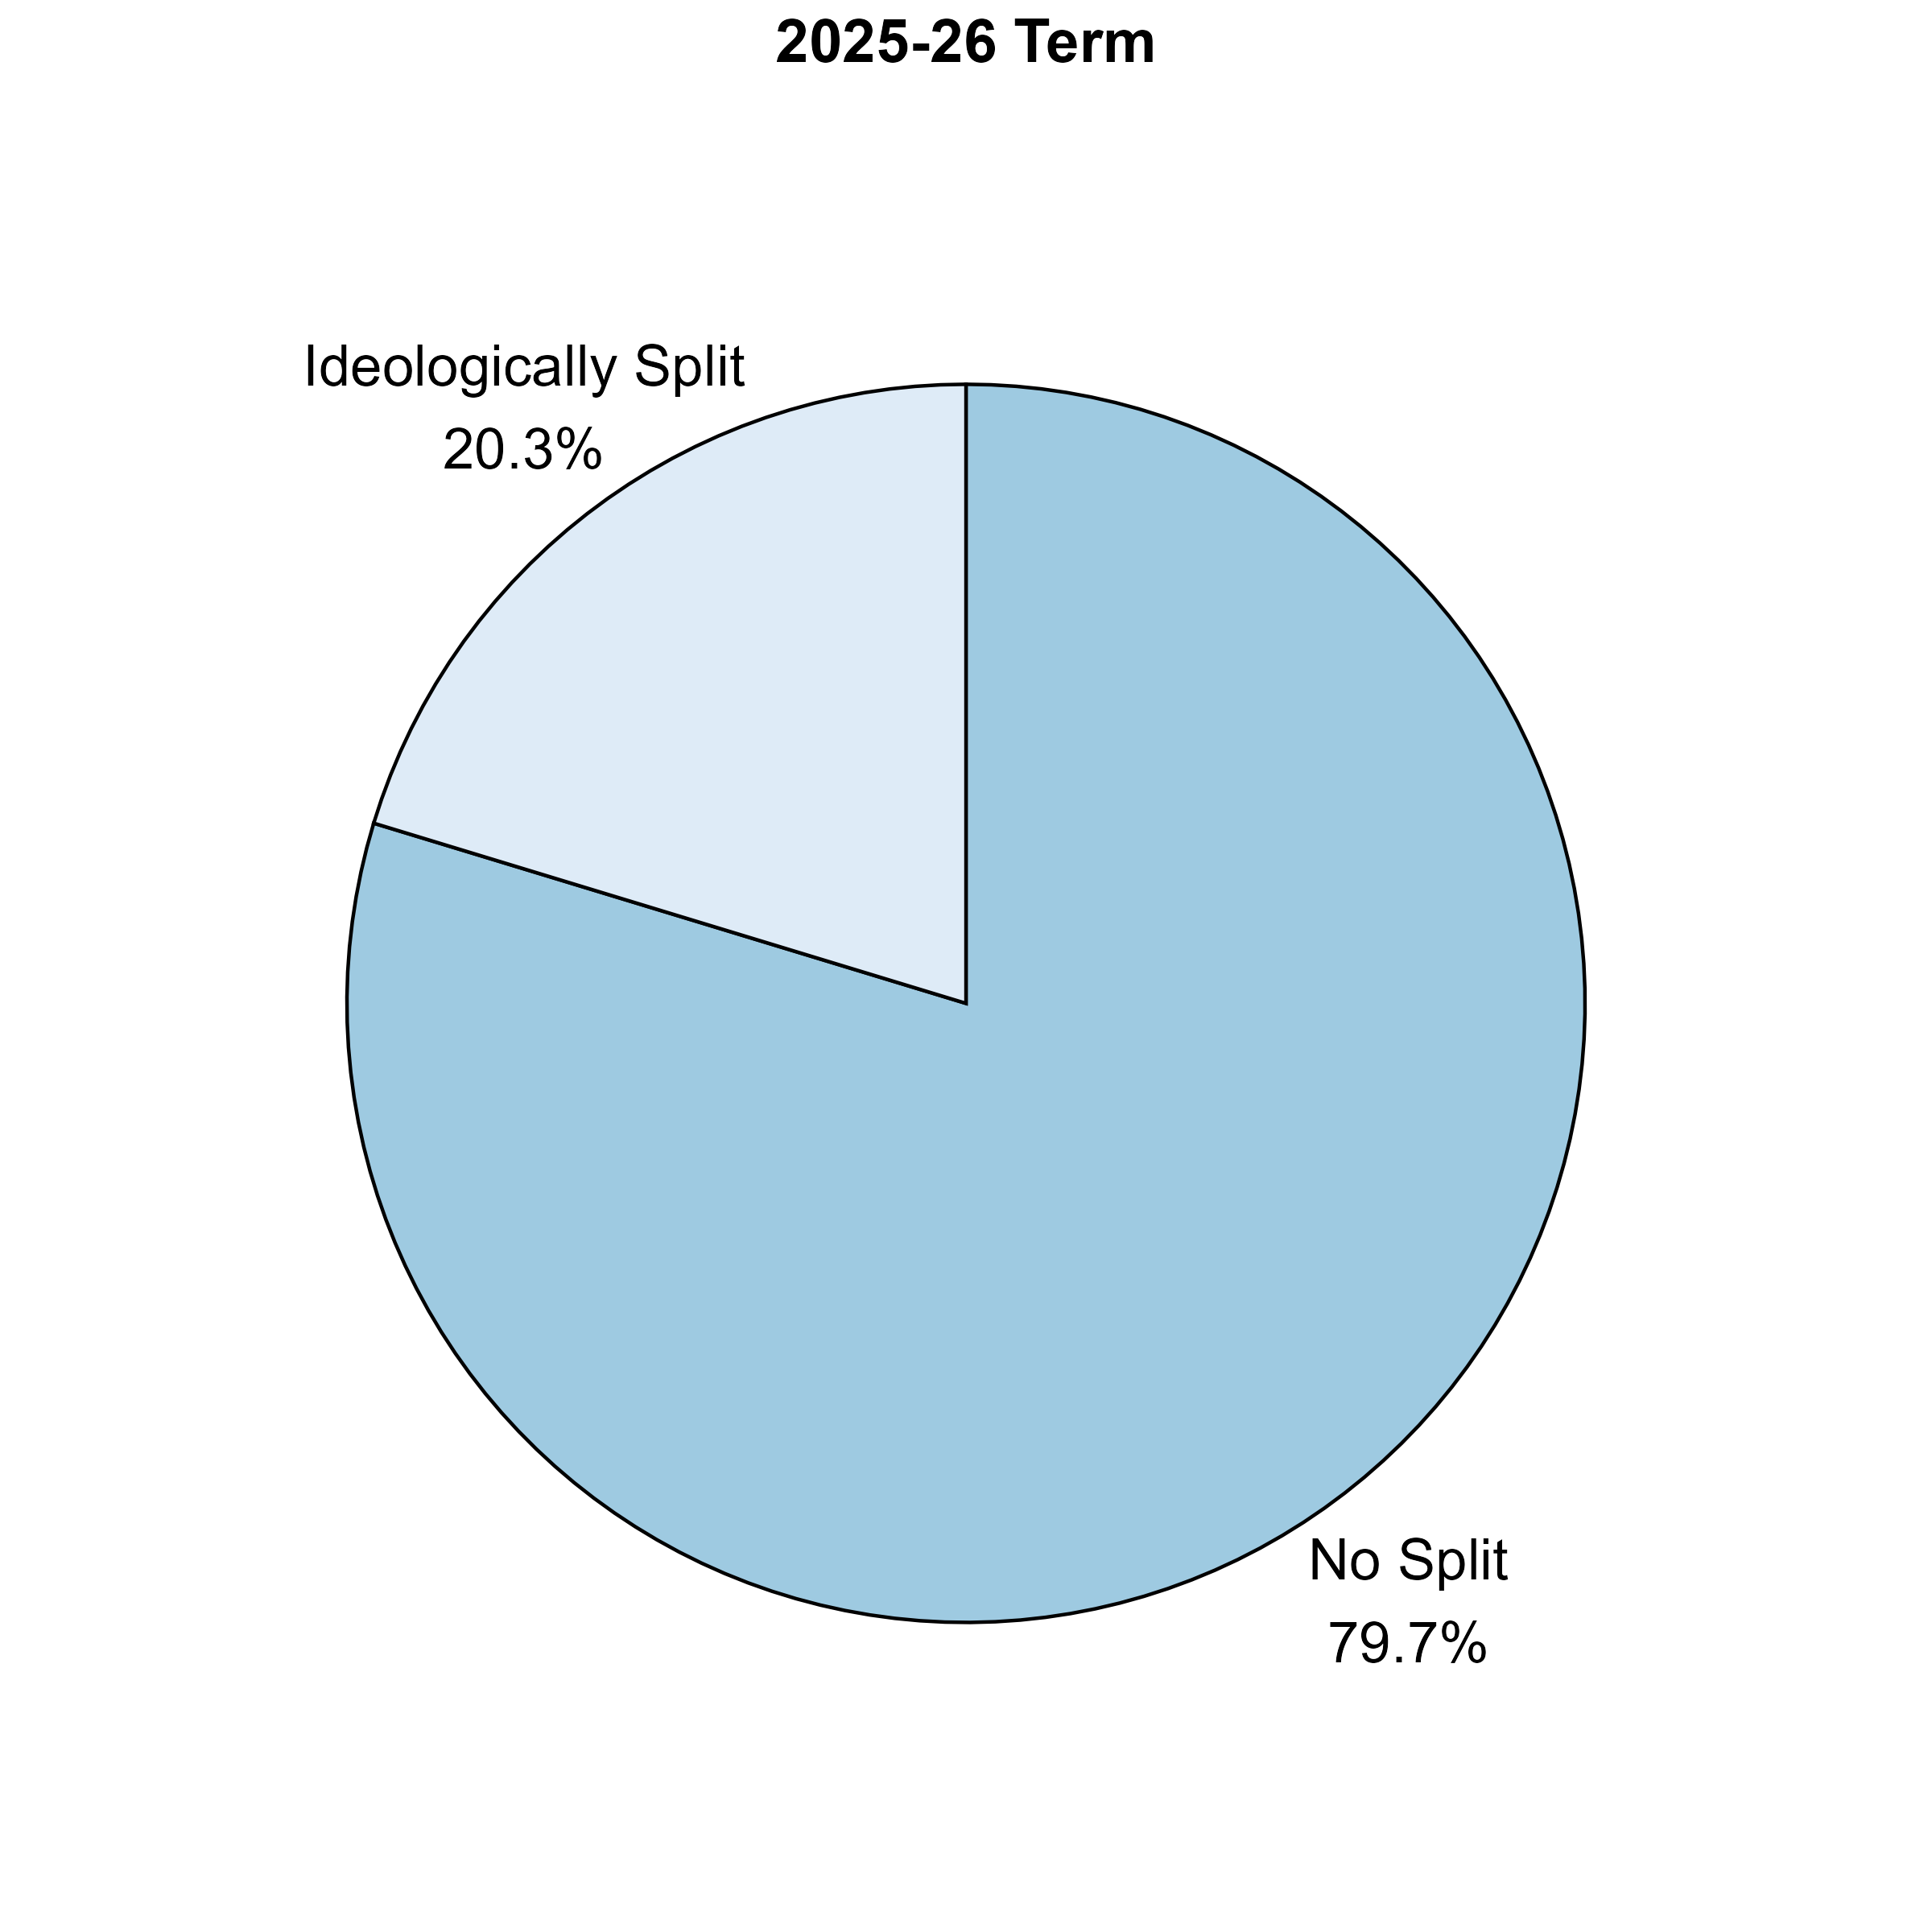
\includegraphics[width=\linewidth]{../../scotusblog_replication/figures/ot25_ideological.png}
    \end{minipage}
\end{figure}
\footernote{
\textbf{Description}: Figures show the percent of cases decided by ideologically split coalitions, consisting of Chief Justice Roberts and Justices Thomas, Alito, Gorsuch, Kavanaugh, and Barrett on one side, and Justices Sotomayor, Kagan, and Jackson on the other.
}
\newpage

W

\section{Closely Divided Cases}

\noindent

\begin{center}
{
\renewcommand{\arraystretch}{3.5}
\begin{table}[!h]
\centering\begingroup\fontsize{11}{13}\selectfont

\begin{tabular}[t]{L{8cm}C{6.5cm}m{12cm}}
\toprule
\multicolumn{1}{c}{\textbf{Condition}} & \multicolumn{1}{c}{\textbf{Percent of All Cases}} & \multicolumn{1}{c}{\textbf{Cases}}\\
\midrule
\textbf{6-3 with Justices Sotomayor, Kagan, and Jackson Dissenting} & 20.3\% & Callais, Zorn, Rutherford, FS Credit, McCarthy, Cisco, Exxon, Landor, Lau, Wolford, Al Otro Lado, Mullin v. Doe\\
\cellcolor[HTML]{F5F5F5}{\textbf{6-3 with Justices Thomas, Alito, and Gorsuch Dissenting}} & \cellcolor[HTML]{F5F5F5}{0\%} & \cellcolor[HTML]{F5F5F5}{}\\
\textbf{Cases with Justices Sotomayor, Kagan, and Jackson All in Dissent} & 22\% & Callais, Zorn, Rutherford, FS Credit, McCarthy, Cisco, Exxon, Landor, Lau, Wolford, Al Otro Lado, Mullin v. Doe, USPS\\
\cellcolor[HTML]{F5F5F5}{\textbf{Cases with Three or More Conservative Justices Dissenting}} & \cellcolor[HTML]{F5F5F5}{10.2\%} & \cellcolor[HTML]{F5F5F5}{Bowe, Pitchford, UMD Medical, Learning Resources, Hamm, Hencely}\\
\bottomrule
\end{tabular}
\endgroup{}
\end{table}}
\end{center}

\newpage

\section{Circuit Scorecard}

\noindent

\begin{center}

\begin{tabular}[t]{>{\centering\arraybackslash}p{5cm}>{\centering\arraybackslash}p{4cm}>{\centering\arraybackslash}p{4cm}>{\centering\arraybackslash}p{4cm}>{\centering\arraybackslash}p{4cm}>{\centering\arraybackslash}p{4cm}}
\toprule
\textbf{Court Below} & \textbf{\# Decided} & \textbf{\# Affirm} & \textbf{\# Reversed} & \textbf{\% Affirmed} & \textbf{\% Reversed}\\
\midrule
\midrule
\textbf{CA1} & 1 & 1 & 0 & 100\% & 0\%\\
\addlinespace[0.5em]
\textbf{\cellcolor[HTML]{F5F5F5}{CA2}} & \cellcolor[HTML]{F5F5F5}{9} & \cellcolor[HTML]{F5F5F5}{3} & \cellcolor[HTML]{F5F5F5}{6} & \cellcolor[HTML]{F5F5F5}{33.3\%} & \cellcolor[HTML]{F5F5F5}{66.7\%}\\
\addlinespace[0.5em]
\textbf{CA3} & 3 & 1 & 2 & 33.3\% & 66.7\%\\
\addlinespace[0.5em]
\textbf{\cellcolor[HTML]{F5F5F5}{CA4}} & \cellcolor[HTML]{F5F5F5}{6} & \cellcolor[HTML]{F5F5F5}{1} & \cellcolor[HTML]{F5F5F5}{5} & \cellcolor[HTML]{F5F5F5}{16.7\%} & \cellcolor[HTML]{F5F5F5}{83.3\%}\\
\addlinespace[0.5em]
\textbf{CA5} & 10 & 3 & 7 & 30\% & 70\%\\
\addlinespace[0.5em]
\textbf{\cellcolor[HTML]{F5F5F5}{CA6}} & \cellcolor[HTML]{F5F5F5}{3} & \cellcolor[HTML]{F5F5F5}{2} & \cellcolor[HTML]{F5F5F5}{1} & \cellcolor[HTML]{F5F5F5}{66.7\%} & \cellcolor[HTML]{F5F5F5}{33.3\%}\\
\addlinespace[0.5em]
\textbf{CA7} & 2 & 0 & 2 & 0\% & 100\%\\
\addlinespace[0.5em]
\textbf{\cellcolor[HTML]{F5F5F5}{CA8}} & \cellcolor[HTML]{F5F5F5}{1} & \cellcolor[HTML]{F5F5F5}{0} & \cellcolor[HTML]{F5F5F5}{1} & \cellcolor[HTML]{F5F5F5}{0\%} & \cellcolor[HTML]{F5F5F5}{100\%}\\
\addlinespace[0.5em]
\textbf{CA9} & 6 & 1 & 5 & 16.7\% & 83.3\%\\
\addlinespace[0.5em]
\textbf{\cellcolor[HTML]{F5F5F5}{CA10}} & \cellcolor[HTML]{F5F5F5}{3} & \cellcolor[HTML]{F5F5F5}{2} & \cellcolor[HTML]{F5F5F5}{1} & \cellcolor[HTML]{F5F5F5}{66.7\%} & \cellcolor[HTML]{F5F5F5}{33.3\%}\\
\addlinespace[0.5em]
\textbf{CA11} & 3 & 0 & 3 & 0\% & 100\%\\
\addlinespace[0.5em]
\textbf{\cellcolor[HTML]{F5F5F5}{CADC}} & \cellcolor[HTML]{F5F5F5}{4} & \cellcolor[HTML]{F5F5F5}{1} & \cellcolor[HTML]{F5F5F5}{3} & \cellcolor[HTML]{F5F5F5}{25\%} & \cellcolor[HTML]{F5F5F5}{75\%}\\
\addlinespace[0.5em]
\textbf{CAFED} & 2 & 1 & 1 & 50\% & 50\%\\
\addlinespace[0.5em]
\midrule
\textbf{\cellcolor[HTML]{F5F5F5}{Total}} & \cellcolor[HTML]{F5F5F5}{53} & \cellcolor[HTML]{F5F5F5}{16} & \cellcolor[HTML]{F5F5F5}{37} & \cellcolor[HTML]{F5F5F5}{30.19\%} & \cellcolor[HTML]{F5F5F5}{69.81\%}\\
\addlinespace[0.5em]
\bottomrule
\end{tabular}\end{center}

\begin{tikzpicture}[remember picture,overlay]

% Box dimensions
\coordinate (boxSW) at ($(current page.south west)+(0.5in,0.10in)$);
\coordinate (boxNE) at ($(current page.south east)+(-0.5in,1.15in)$);

% Draw box
\filldraw[
  fill=dispatchBlue!8,
  draw=dispatchBlue,
  line width=1.2pt,
  rounded corners=6pt
]
(boxSW) rectangle (boxNE);

% Text
\node[
anchor=center,
text width=11.5in,
align=left,
font=\footnotesize
]
at ($(boxSW)!0.5!(boxNE)$)
{

\textbf{Description}: Table reflects the rates of affirmance and reversal for cases decided during OT25 that emerged from the U.S. Courts of Appeals.  \par 

\vspace{4mm}

\textbf{Notes}: (1) We treat consolidated cases emerging from the same lower court as single entries. (2) Decisions that were granted review but subsequently dismissed (as improvidently granted) are omitted. (3) Table further includes the following decisions from consolidated proceedings: 25-567 (CA2, Affirm); 25-1084 (CADC, Reverse); 25-250 (CAFED, Affirm)
};

\end{tikzpicture}

\newpage

\section{Opinions Authored by Each
Justice}\label{opinions-authored-by-each-justice}

\vspace{-0.75cm}\begingroup\fontsize{8}{10}\selectfont

\begin{longtable}[t]{>{\centering\arraybackslash}p{3cm}>{\centering\arraybackslash}p{3cm}>{\centering\arraybackslash}p{3cm}>{\centering\arraybackslash}p{3cm}>{\centering\arraybackslash}p{3cm}>{\centering\arraybackslash}p{3cm}>{\centering\arraybackslash}p{3cm}>{\centering\arraybackslash}p{3cm}>{\centering\arraybackslash}p{3cm}}
\toprule
\multicolumn{9}{c}{\normalsize \textbf{Majority Opinions}} \\
\cmidrule(l{3pt}r{3pt}){1-9}
\begingroup\fontsize{9}{11}\selectfont \textbf{Roberts}\endgroup & \begingroup\fontsize{9}{11}\selectfont \textbf{Thomas}\endgroup & \begingroup\fontsize{9}{11}\selectfont \textbf{Alito}\endgroup & \begingroup\fontsize{9}{11}\selectfont \textbf{Sotomayor}\endgroup & \begingroup\fontsize{9}{11}\selectfont \textbf{Kagan}\endgroup & \begingroup\fontsize{9}{11}\selectfont \textbf{Gorsuch}\endgroup & \begingroup\fontsize{9}{11}\selectfont \textbf{Kavanaugh}\endgroup & \begingroup\fontsize{9}{11}\selectfont \textbf{Barrett}\endgroup & \begingroup\fontsize{9}{11}\selectfont \textbf{Jackson}\endgroup\\
\midrule
\endfirsthead
\multicolumn{9}{@{}l}{\textit{(continued)}}\\
\toprule
\multicolumn{9}{c}{\normalsize \textbf{Majority Opinions}} \\
\cmidrule(l{3pt}r{3pt}){1-9}
\begingroup\fontsize{9}{11}\selectfont \textbf{Roberts}\endgroup & \begingroup\fontsize{9}{11}\selectfont \textbf{Thomas}\endgroup & \begingroup\fontsize{9}{11}\selectfont \textbf{Alito}\endgroup & \begingroup\fontsize{9}{11}\selectfont \textbf{Sotomayor}\endgroup & \begingroup\fontsize{9}{11}\selectfont \textbf{Kagan}\endgroup & \begingroup\fontsize{9}{11}\selectfont \textbf{Gorsuch}\endgroup & \begingroup\fontsize{9}{11}\selectfont \textbf{Kavanaugh}\endgroup & \begingroup\fontsize{9}{11}\selectfont \textbf{Barrett}\endgroup & \begingroup\fontsize{9}{11}\selectfont \textbf{Jackson}\endgroup\\
\midrule
\endhead

\endfoot

\endlastfoot
\cellcolor{gray!10}{Bost} & \cellcolor{gray!10}{Plaquemines Parish} & \cellcolor{gray!10}{Coney Island Auto} & \cellcolor{gray!10}{Bowe} & \cellcolor{gray!10}{Case} & \cellcolor{gray!10}{Chiles} & \cellcolor{gray!10}{Ellingburg} & \cellcolor{gray!10}{Berk} & \cellcolor{gray!10}{Barrett}\\
Learning Resources & Cox & Callais & Enbridge & GEO Group & First Choice & Pitchford & Montgomery & Urias-Orellana\\
\cellcolor{gray!10}{AT\&T} & \cellcolor{gray!10}{Hencely} & \cellcolor{gray!10}{Pung} & \cellcolor{gray!10}{Galette} & \cellcolor{gray!10}{Olivier} & \cellcolor{gray!10}{Rico} & \cellcolor{gray!10}{Exxon} & \cellcolor{gray!10}{Fernandez} & \cellcolor{gray!10}{Villarreal}\\
 & USPS & Wolford & Hain Celestial Grp. & Abouammo & Flowers Foods & Monsanto & Rutherford & IAM Pension Fund\\
\cellcolor{gray!10}{} & \cellcolor{gray!10}{Havana Docks} & \cellcolor{gray!10}{Al Otro Lado} & \cellcolor{gray!10}{Jules} & \cellcolor{gray!10}{Hunter} & \cellcolor{gray!10}{Sripetch} & \cellcolor{gray!10}{} & \cellcolor{gray!10}{FS Credit} & \cellcolor{gray!10}{Hikma}\\
 & Lau & Mullin v. Doe & UMD Medical &  & Hemani &  & Cisco & Keathley\\
\cellcolor{gray!10}{} & \cellcolor{gray!10}{} & \cellcolor{gray!10}{} & \cellcolor{gray!10}{} & \cellcolor{gray!10}{} & \cellcolor{gray!10}{Landor} & \cellcolor{gray!10}{} & \cellcolor{gray!10}{} & \cellcolor{gray!10}{}\\*
\end{longtable}
\endgroup{}\vspace{-0.75cm}\begingroup\fontsize{8}{10}\selectfont

\begin{longtable}[t]{>{\centering\arraybackslash}p{3cm}>{\centering\arraybackslash}p{3cm}>{\centering\arraybackslash}p{3cm}>{\centering\arraybackslash}p{3cm}>{\centering\arraybackslash}p{3cm}>{\centering\arraybackslash}p{3cm}>{\centering\arraybackslash}p{3cm}>{\centering\arraybackslash}p{3cm}>{\centering\arraybackslash}p{3cm}}
\toprule
\multicolumn{9}{c}{\normalsize \textbf{Concurring Opinions}} \\
\cmidrule(l{3pt}r{3pt}){1-9}
\begingroup\fontsize{9}{11}\selectfont \textbf{Roberts}\endgroup & \begingroup\fontsize{9}{11}\selectfont \textbf{Thomas}\endgroup & \begingroup\fontsize{9}{11}\selectfont \textbf{Alito}\endgroup & \begingroup\fontsize{9}{11}\selectfont \textbf{Sotomayor}\endgroup & \begingroup\fontsize{9}{11}\selectfont \textbf{Kagan}\endgroup & \begingroup\fontsize{9}{11}\selectfont \textbf{Gorsuch}\endgroup & \begingroup\fontsize{9}{11}\selectfont \textbf{Kavanaugh}\endgroup & \begingroup\fontsize{9}{11}\selectfont \textbf{Barrett}\endgroup & \begingroup\fontsize{9}{11}\selectfont \textbf{Jackson}\endgroup\\
\midrule
\endfirsthead
\multicolumn{9}{@{}l}{\textit{(continued)}}\\
\toprule
\multicolumn{9}{c}{\normalsize \textbf{Concurring Opinions}} \\
\cmidrule(l{3pt}r{3pt}){1-9}
\begingroup\fontsize{9}{11}\selectfont \textbf{Roberts}\endgroup & \begingroup\fontsize{9}{11}\selectfont \textbf{Thomas}\endgroup & \begingroup\fontsize{9}{11}\selectfont \textbf{Alito}\endgroup & \begingroup\fontsize{9}{11}\selectfont \textbf{Sotomayor}\endgroup & \begingroup\fontsize{9}{11}\selectfont \textbf{Kagan}\endgroup & \begingroup\fontsize{9}{11}\selectfont \textbf{Gorsuch}\endgroup & \begingroup\fontsize{9}{11}\selectfont \textbf{Kavanaugh}\endgroup & \begingroup\fontsize{9}{11}\selectfont \textbf{Barrett}\endgroup & \begingroup\fontsize{9}{11}\selectfont \textbf{Jackson}\endgroup\\
\midrule
\endhead

\endfoot

\endlastfoot
\cellcolor{gray!10}{} & \cellcolor{gray!10}{Ellingburg} & \cellcolor{gray!10}{GEO Group} & \cellcolor{gray!10}{Case} & \cellcolor{gray!10}{Chiles} & \cellcolor{gray!10}{Barrett} & \cellcolor{gray!10}{Montgomery} & \cellcolor{gray!10}{Bost} & \cellcolor{gray!10}{Berk}\\
 & GEO Group & Villarreal & Coney Island Auto & Learning Resources & Case & Hunter & Learning Resources & Bowe\\
\cellcolor{gray!10}{} & \cellcolor{gray!10}{Hain Celestial Grp.} & \cellcolor{gray!10}{Hemani} & \cellcolor{gray!10}{Cox} & \cellcolor{gray!10}{} & \cellcolor{gray!10}{Learning Resources} & \cellcolor{gray!10}{} & \cellcolor{gray!10}{Hunter} & \cellcolor{gray!10}{Plaquemines Parish}\\
 & Callais &  & Havana Docks &  & Hunter &  & Wolford & Learning Resources\\
\cellcolor{gray!10}{} & \cellcolor{gray!10}{Villarreal} & \cellcolor{gray!10}{} & \cellcolor{gray!10}{Hamm} & \cellcolor{gray!10}{} & \cellcolor{gray!10}{} & \cellcolor{gray!10}{} & \cellcolor{gray!10}{} & \cellcolor{gray!10}{Hemani}\\
 & Margolin &  & Fernandez &  &  &  &  & Cisco\\
\cellcolor{gray!10}{} & \cellcolor{gray!10}{Sripetch} & \cellcolor{gray!10}{} & \cellcolor{gray!10}{Keathley} & \cellcolor{gray!10}{} & \cellcolor{gray!10}{} & \cellcolor{gray!10}{} & \cellcolor{gray!10}{} & \cellcolor{gray!10}{}\\
 & Keathley &  & Pung &  &  &  &  & \\
\cellcolor{gray!10}{} & \cellcolor{gray!10}{Hemani} & \cellcolor{gray!10}{} & \cellcolor{gray!10}{} & \cellcolor{gray!10}{} & \cellcolor{gray!10}{} & \cellcolor{gray!10}{} & \cellcolor{gray!10}{} & \cellcolor{gray!10}{}\\
 & UMD Medical &  &  &  &  &  &  & \\
\cellcolor{gray!10}{} & \cellcolor{gray!10}{Pung} & \cellcolor{gray!10}{} & \cellcolor{gray!10}{} & \cellcolor{gray!10}{} & \cellcolor{gray!10}{} & \cellcolor{gray!10}{} & \cellcolor{gray!10}{} & \cellcolor{gray!10}{}\\
 & Monsanto &  &  &  &  &  &  & \\
\cellcolor{gray!10}{} & \cellcolor{gray!10}{Al Otro Lado} & \cellcolor{gray!10}{} & \cellcolor{gray!10}{} & \cellcolor{gray!10}{} & \cellcolor{gray!10}{} & \cellcolor{gray!10}{} & \cellcolor{gray!10}{} & \cellcolor{gray!10}{}\\
 & Mullin v. Doe &  &  &  &  &  &  & \\*
\end{longtable}
\endgroup{}\vspace{-0.75cm}\begingroup\fontsize{8}{10}\selectfont

\begin{longtable}[t]{>{\centering\arraybackslash}p{3cm}>{\centering\arraybackslash}p{3cm}>{\centering\arraybackslash}p{3cm}>{\centering\arraybackslash}p{3cm}>{\centering\arraybackslash}p{3cm}>{\centering\arraybackslash}p{3cm}>{\centering\arraybackslash}p{3cm}>{\centering\arraybackslash}p{3cm}>{\centering\arraybackslash}p{3cm}}
\toprule
\multicolumn{9}{c}{\normalsize \textbf{Dissenting Opinions}} \\
\cmidrule(l{3pt}r{3pt}){1-9}
\begingroup\fontsize{9}{11}\selectfont \textbf{Roberts}\endgroup & \begingroup\fontsize{9}{11}\selectfont \textbf{Thomas}\endgroup & \begingroup\fontsize{9}{11}\selectfont \textbf{Alito}\endgroup & \begingroup\fontsize{9}{11}\selectfont \textbf{Sotomayor}\endgroup & \begingroup\fontsize{9}{11}\selectfont \textbf{Kagan}\endgroup & \begingroup\fontsize{9}{11}\selectfont \textbf{Gorsuch}\endgroup & \begingroup\fontsize{9}{11}\selectfont \textbf{Kavanaugh}\endgroup & \begingroup\fontsize{9}{11}\selectfont \textbf{Barrett}\endgroup & \begingroup\fontsize{9}{11}\selectfont \textbf{Jackson}\endgroup\\
\midrule
\endfirsthead
\multicolumn{9}{@{}l}{\textit{(continued)}}\\
\toprule
\multicolumn{9}{c}{\normalsize \textbf{Dissenting Opinions}} \\
\cmidrule(l{3pt}r{3pt}){1-9}
\begingroup\fontsize{9}{11}\selectfont \textbf{Roberts}\endgroup & \begingroup\fontsize{9}{11}\selectfont \textbf{Thomas}\endgroup & \begingroup\fontsize{9}{11}\selectfont \textbf{Alito}\endgroup & \begingroup\fontsize{9}{11}\selectfont \textbf{Sotomayor}\endgroup & \begingroup\fontsize{9}{11}\selectfont \textbf{Kagan}\endgroup & \begingroup\fontsize{9}{11}\selectfont \textbf{Gorsuch}\endgroup & \begingroup\fontsize{9}{11}\selectfont \textbf{Kavanaugh}\endgroup & \begingroup\fontsize{9}{11}\selectfont \textbf{Barrett}\endgroup & \begingroup\fontsize{9}{11}\selectfont \textbf{Jackson}\endgroup\\
\midrule
\endhead

\endfoot
\bottomrule
\endlastfoot
\cellcolor{gray!10}{} & \cellcolor{gray!10}{Learning Resources} & \cellcolor{gray!10}{Hencely} & \cellcolor{gray!10}{USPS} & \cellcolor{gray!10}{Callais} & \cellcolor{gray!10}{Bowe} & \cellcolor{gray!10}{Learning Resources} & \cellcolor{gray!10}{UMD Medical} & \cellcolor{gray!10}{Bost}\\
 & Hamm & Rico & Zorn & Havana Docks & Pitchford &  &  & Chiles\\
\cellcolor{gray!10}{} & \cellcolor{gray!10}{Whitton} & \cellcolor{gray!10}{Hamm} & \cellcolor{gray!10}{Rutherford} & \cellcolor{gray!10}{FS Credit} & \cellcolor{gray!10}{} & \cellcolor{gray!10}{} & \cellcolor{gray!10}{} & \cellcolor{gray!10}{R.W.}\\
 & AT\&T &  & Cisco & Exxon &  &  &  & Fernandez\\
\cellcolor{gray!10}{} & \cellcolor{gray!10}{Hunter} & \cellcolor{gray!10}{} & \cellcolor{gray!10}{Al Otro Lado} & \cellcolor{gray!10}{Wolford} & \cellcolor{gray!10}{} & \cellcolor{gray!10}{} & \cellcolor{gray!10}{} & \cellcolor{gray!10}{FS Credit}\\
 &  &  &  & Mullin v. Doe &  &  &  & Landor\\
\cellcolor{gray!10}{} & \cellcolor{gray!10}{} & \cellcolor{gray!10}{} & \cellcolor{gray!10}{} & \cellcolor{gray!10}{} & \cellcolor{gray!10}{} & \cellcolor{gray!10}{} & \cellcolor{gray!10}{} & \cellcolor{gray!10}{Lau}\\
 &  &  &  &  &  &  &  & Monsanto\\
\cellcolor{gray!10}{} & \cellcolor{gray!10}{} & \cellcolor{gray!10}{} & \cellcolor{gray!10}{} & \cellcolor{gray!10}{} & \cellcolor{gray!10}{} & \cellcolor{gray!10}{} & \cellcolor{gray!10}{} & \cellcolor{gray!10}{Wolford}\\
 &  &  &  &  &  &  &  & Al Otro Lado\\*
\end{longtable}
\endgroup{}

\newpage

\section*{Opinions Authored by Each Justice (Cont.)}
\begin{figure}[h!]
    \centering
      
\includegraphics[width=0.75\linewidth]{../../scotusblog_replication/figures/opinions_by_justice.png}
\end{figure}

\footernote{
\textbf{Description}: Figure shows the volume and proportion of opinions (by type) authored by each justice during the 2025 term.

}
\newpage

\section{Days Between Oral Argument \& Opinion}

\vspace{-0.75cm}

\begin{figure}[H]
\centering

%------------------------------------
% TOP ROW
%------------------------------------

\begin{minipage}[t]{0.25\textwidth}
\centering
\vspace{0pt}

 
\begin{tabular}[t]{>{}cc}
\toprule
\textbf{Justice} & \textbf{Average Days Between Argument and Opinion}\\
\midrule
\textbf{Roberts} & 84.00\\
\textbf{\cellcolor[HTML]{F5F5F5}{Thomas}} & \cellcolor[HTML]{F5F5F5}{112.17}\\
\textbf{Alito} & 117.17\\
\textbf{\cellcolor[HTML]{F5F5F5}{Sotomayor}} & \cellcolor[HTML]{F5F5F5}{68.83}\\
\textbf{Kagan} & 98.00\\
\textbf{\cellcolor[HTML]{F5F5F5}{Gorsuch}} & \cellcolor[HTML]{F5F5F5}{130.57}\\
\textbf{Kavanaugh} & 84.75\\
\textbf{\cellcolor[HTML]{F5F5F5}{Barrett}} & \cellcolor[HTML]{F5F5F5}{136.00}\\
\textbf{Jackson} & 96.00\\
\bottomrule
\end{tabular} 

\end{minipage}
\hspace{0.15cm}
\begin{minipage}[t]{0.7\textwidth}
\raggedleft
\vspace{0pt}

 
\begin{tabular}[t]{>{}c>{}cccccc}
\toprule
\textbf{} & \textbf{Case} & \textbf{Days} & \textbf{Author} & \textbf{Vote} & \textbf{Argued} & \textbf{Decided}\\
\midrule
\textbf{} & \em{Hikma} & 37 & Jackson & (9-0) & 04/29/2026 & 06/04/2026\\
\textbf{\cellcolor[HTML]{F5F5F5}{}} & \em{\cellcolor[HTML]{F5F5F5}{AT\&T}} & \cellcolor[HTML]{F5F5F5}{45} & \cellcolor[HTML]{F5F5F5}{Roberts} & \cellcolor[HTML]{F5F5F5}{(8-1)} & \cellcolor[HTML]{F5F5F5}{04/21/2026} & \cellcolor[HTML]{F5F5F5}{06/04/2026}\\
\textbf{Shortest} & \em{Sripetch} & 46 & Gorsuch & (9-0) & 04/20/2026 & 06/04/2026\\
\textbf{\cellcolor[HTML]{F5F5F5}{}} & \em{\cellcolor[HTML]{F5F5F5}{Jules}} & \cellcolor[HTML]{F5F5F5}{46} & \cellcolor[HTML]{F5F5F5}{Sotomayor} & \cellcolor[HTML]{F5F5F5}{(9-0)} & \cellcolor[HTML]{F5F5F5}{03/30/2026} & \cellcolor[HTML]{F5F5F5}{05/14/2026}\\
\textbf{} & \em{Galette} & 50 & Sotomayor & (9-0) & 01/14/2026 & 03/04/2026\\
\midrule
\textbf{\cellcolor[HTML]{F5F5F5}{}} & \em{\cellcolor[HTML]{F5F5F5}{Landor}} & \cellcolor[HTML]{F5F5F5}{226} & \cellcolor[HTML]{F5F5F5}{Gorsuch} & \cellcolor[HTML]{F5F5F5}{(6-3)} & \cellcolor[HTML]{F5F5F5}{11/10/2025} & \cellcolor[HTML]{F5F5F5}{06/23/2026}\\
\textbf{} & \em{Fernandez} & 198 & Barrett & (8-1) & 11/12/2025 & 05/28/2026\\
\textbf{\cellcolor[HTML]{F5F5F5}{Longest}} & \em{\cellcolor[HTML]{F5F5F5}{Rutherford}} & \cellcolor[HTML]{F5F5F5}{198} & \cellcolor[HTML]{F5F5F5}{Barrett} & \cellcolor[HTML]{F5F5F5}{(6-3)} & \cellcolor[HTML]{F5F5F5}{11/12/2025} & \cellcolor[HTML]{F5F5F5}{05/28/2026}\\
\textbf{} & \em{Callais} & 197 & Alito & (6-3) & 10/15/2025 & 04/29/2026\\
\textbf{\cellcolor[HTML]{F5F5F5}{}} & \em{\cellcolor[HTML]{F5F5F5}{FS Credit}} & \cellcolor[HTML]{F5F5F5}{184} & \cellcolor[HTML]{F5F5F5}{Barrett} & \cellcolor[HTML]{F5F5F5}{(6-3)} & \cellcolor[HTML]{F5F5F5}{12/10/2025} & \cellcolor[HTML]{F5F5F5}{06/11/2026}\\
\bottomrule
\end{tabular} 

\end{minipage}

%------------------------------------
% spacing
%------------------------------------

\vspace{0.8cm}

%------------------------------------
% BOTTOM ROW
%------------------------------------

\begin{minipage}[t]{0.60\textwidth}
\centering
\vspace{0pt}


\includegraphics[width=0.75\linewidth]{../../scotusblog_replication/figures/days_elapsed_figure.png}

\end{minipage}
\hfill
\begin{minipage}[t]{0.35\textwidth}
\vspace{0pt}


\hspace{-2cm}
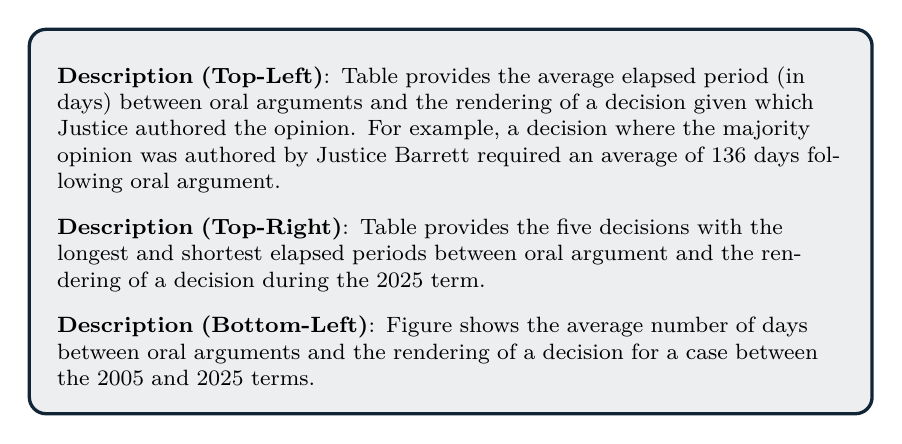
\begin{tikzpicture}[outer sep=0pt,inner sep=0pt]
\node[
fill=dispatchBlue!8,
draw=dispatchBlue,
line width=1.2pt,
rounded corners=6pt,
inner sep=10pt,
text width=10cm,
align=left,
font=\footnotesize, 
]{


 
\textbf{Description (Top-Left)}: Table provides the average elapsed period (in days) between oral arguments and the rendering of a decision given which Justice authored the opinion. For example, a decision where the majority opinion was authored by Justice Barrett required an average of  136  days following oral argument.  \par \vspace{2.5mm}

\textbf{Description (Top-Right)}: Table provides the five decisions with the longest and shortest elapsed periods between oral argument and the rendering of a decision during the 2025 term.  \par \vspace{2.5mm}

\textbf{Description (Bottom-Left)}: Figure shows the average number of days between oral arguments and the rendering of a decision for a case between the 2005 and 2025 terms. \par \vspace{2.5mm}

 


};
\end{tikzpicture}


\end{minipage}

\end{figure}

\vspace{-10mm}

\section{Opinion Lengths}

\begingroup\fontsize{10}{12}\selectfont

\begin{longtable}[t]{>{}ccc>{\centering\arraybackslash}p{6cm}ccc}
\toprule
\multicolumn{1}{c}{\textbf{}} & \multicolumn{1}{c}{\textbf{Case}} & \multicolumn{1}{c}{\textbf{Opinion Type (Total Opinions)}} & \multicolumn{1}{c}{\textbf{Author(s)}} & \multicolumn{1}{c}{\textbf{Vote}} & \multicolumn{1}{c}{\textbf{Word Count}} & \multicolumn{1}{c}{\textbf{Decided}}\\
\midrule
\endfirsthead
\multicolumn{7}{@{}l}{\textit{(continued)}}\\
\toprule
\multicolumn{1}{c}{\textbf{}} & \multicolumn{1}{c}{\textbf{Case}} & \multicolumn{1}{c}{\textbf{Opinion Type (Total Opinions)}} & \multicolumn{1}{c}{\textbf{Author(s)}} & \multicolumn{1}{c}{\textbf{Vote}} & \multicolumn{1}{c}{\textbf{Word Count}} & \multicolumn{1}{c}{\textbf{Decided}}\\
\midrule
\endhead

\endfoot
\bottomrule
\endlastfoot
\cellcolor{white}{\textbf{\cellcolor{gray!10}{}}} & \cellcolor{gray!10}{Zorn} & \cellcolor{gray!10}{Per Curiam} & \cellcolor{gray!10}{Per Curiam} & \cellcolor{gray!10}{(6-3)} & \cellcolor{gray!10}{209} & \cellcolor{gray!10}{3/23/2026}\\
\cellcolor{white}{\textbf{Shortest}} & Coney Island Auto & Concurrence & Sotomayor & (9-0) & 211 & 1/20/2026\\
\cellcolor{white}{\textbf{\cellcolor{gray!10}{(Individual Opinions)}}} & \cellcolor{gray!10}{Dynamic PT} & \cellcolor{gray!10}{Per Curiam} & \cellcolor{gray!10}{Per Curiam} & \cellcolor{gray!10}{(9-0)} & \cellcolor{gray!10}{228} & \cellcolor{gray!10}{12/8/2025}\\
\cellcolor{white}{\textbf{}} & Callais & Concurrence & Thomas & (6-3) & 315 & 4/29/2026\\
\cellcolor{white}{\textbf{\cellcolor{gray!10}{}}} & \cellcolor{gray!10}{GEO Group} & \cellcolor{gray!10}{Concurrence} & \cellcolor{gray!10}{Thomas} & \cellcolor{gray!10}{(9-0)} & \cellcolor{gray!10}{377} & \cellcolor{gray!10}{2/25/2026}\\
\midrule
\cellcolor{white}{\textbf{}} & Learning Resources & Dissent & Kavanaugh & (6-3) & 17,030 & 2/20/2026\\
\cellcolor{white}{\textbf{\cellcolor{gray!10}{Longest}}} & \cellcolor{gray!10}{Learning Resources} & \cellcolor{gray!10}{Concurrence} & \cellcolor{gray!10}{Gorsuch} & \cellcolor{gray!10}{(6-3)} & \cellcolor{gray!10}{14,065} & \cellcolor{gray!10}{2/20/2026}\\
\cellcolor{white}{\textbf{(Individual Opinions)}} & Callais & Dissent & Kagan & (6-3) & 13,905 & 4/29/2026\\
\cellcolor{white}{\textbf{\cellcolor{gray!10}{}}} & \cellcolor{gray!10}{Callais} & \cellcolor{gray!10}{Majority Opinion} & \cellcolor{gray!10}{Alito} & \cellcolor{gray!10}{(6-3)} & \cellcolor{gray!10}{10,237} & \cellcolor{gray!10}{4/29/2026}\\
\cellcolor{white}{\textbf{}} & Chiles & Dissent & Jackson & (8-1) & 9,047 & 3/31/2026\\
\midrule
\cellcolor{white}{\textbf{\cellcolor{gray!10}{}}} & \cellcolor{gray!10}{Learning Resources} & \cellcolor{gray!10}{(7 Opinions)} & \cellcolor{gray!10}{Roberts; Gorsuch; Barrett; Kagan; Jackson; Thomas; Kavanaugh} & \cellcolor{gray!10}{(6-3)} & \cellcolor{gray!10}{44,972} & \cellcolor{gray!10}{2/20/2026}\\
\cellcolor{white}{\textbf{}} & Callais & (3 Opinions) & Alito; Thomas; Kagan & (6-3) & 24,457 & 4/29/2026\\
\cellcolor{white}{\textbf{\cellcolor{gray!10}{}}} & \cellcolor{gray!10}{Hamm} & \cellcolor{gray!10}{(4 Opinions)} & \cellcolor{gray!10}{Per Curiam; Sotomayor; Thomas; Alito} & \cellcolor{gray!10}{(5-4)} & \cellcolor{gray!10}{17,710} & \cellcolor{gray!10}{5/21/2026}\\
\cellcolor{white}{\textbf{}} & Chiles & (3 Opinions) & Gorsuch; Kagan; Jackson & (8-1) & 16,958 & 3/31/2026\\
\cellcolor{white}{\textbf{\cellcolor{gray!10}{Longest}}} & \cellcolor{gray!10}{Bowe} & \cellcolor{gray!10}{(3 Opinions)} & \cellcolor{gray!10}{Sotomayor; Jackson; Gorsuch} & \cellcolor{gray!10}{(5-4)} & \cellcolor{gray!10}{15,423} & \cellcolor{gray!10}{1/9/2026}\\
\cellcolor{white}{\textbf{(Total Combined)}} & Hencely & (2 Opinions) & Thomas; Alito & (6-3) & 9,430 & 4/22/2026\\
\cellcolor{white}{\textbf{\cellcolor{gray!10}{}}} & \cellcolor{gray!10}{USPS} & \cellcolor{gray!10}{(2 Opinions)} & \cellcolor{gray!10}{Thomas; Sotomayor} & \cellcolor{gray!10}{(5-4)} & \cellcolor{gray!10}{7,928} & \cellcolor{gray!10}{2/24/2026}\\
\cellcolor{white}{\textbf{}} & Bost & (2 Opinions) & Roberts; Jackson & (7-2) & 7,868 & 1/14/2026\\
\cellcolor{white}{\textbf{\cellcolor{gray!10}{}}} & \cellcolor{gray!10}{Havana Docks} & \cellcolor{gray!10}{(3 Opinions)} & \cellcolor{gray!10}{Thomas; Sotomayor; Kagan} & \cellcolor{gray!10}{(8-1)} & \cellcolor{gray!10}{7,452} & \cellcolor{gray!10}{5/21/2026}\\
\cellcolor{white}{\textbf{}} & Villarreal & (3 Opinions) & Jackson; Alito; Thomas & (9-0) & 7,218 & 2/25/2026\\*
\end{longtable}
\endgroup{}

\begin{tikzpicture}[remember picture,overlay]

% Box dimensions
\coordinate (boxSW) at ($(current page.south west)+(0.5in,0.10in)$);
\coordinate (boxNE) at ($(current page.south east)+(-0.5in,1.9in)$);

% Draw box
\filldraw[
  fill=dispatchBlue!8,
  draw=dispatchBlue,
  line width=1.2pt,
  rounded corners=6pt
]
(boxSW) rectangle (boxNE);

% Text
\node[
anchor=center,
text width=11.5in,
align=left,
font=\footnotesize
]
at ($(boxSW)!0.5!(boxNE)$)
{

\textbf{Descriptions}: \par \vspace{2.5mm} 

\textbf{Longest (Total Combined)}: Table represents cases with the largest total word count combined across the published majority and separate opinions. For example, the 7 opinions published in \emph{Learning Resources, Inc. v. Trump} (24-1287) totaled approximately 45,000 words -- which included both a dissent filed by Justice Kavanaugh ($\approx$ 17,000 words), as well as a separate concurrence filed by Justice Gorsuch ($\approx$ 14,000 words). \par \vspace{2.5mm}

\textbf{Shortest (Longest) (Individual Opinions)}: Table represents the shortest (longest) opinions filed by individual justices (or per curiam). For example, Justice Kagan's dissenting opinion in \emph{Louisiana v. Callais} represents one of the longest individual opinions this term at approximately 13,900 words. \par \vspace{2.5mm}

\textbf{Notes}: (1) Cases that were dismissed as improvidently granted (e.g., \emph{Hamm v. Smith}) are omitted from \emph{smallest individual opinions}. 


};

\end{tikzpicture}

\newpage

\section{Opinion Lengths (Cont.)}

\begin{figure}[H]
\centering

%------------------------------------
% TOP ROW
%------------------------------------

\hspace*{0.5cm}
\begin{minipage}[t]{0.35\textwidth}
\centering
\vspace{0pt}
{\centering
\small\textbf{Average Opinion Length by Authoring Justice}\par
\vspace{0.2cm}
}
 \begingroup\fontsize{10}{12}\selectfont

\begin{longtable}[t]{>{\centering\arraybackslash}p{5cm}>{\centering\arraybackslash}p{5cm}}
\toprule
\textbf{Justice} & \textbf{Words}\\
\midrule
\endfirsthead
\multicolumn{2}{@{}l}{\textit{(continued)}}\\
\toprule
\textbf{Justice} & \textbf{Words}\\
\midrule
\endhead

\endfoot
\bottomrule
\endlastfoot
\cellcolor{gray!10}{Roberts} & \cellcolor{gray!10}{\ensuremath{\approx} 4000 Words}\\
Thomas & \ensuremath{\approx} 3100 Words\\
\cellcolor{gray!10}{Alito} & \cellcolor{gray!10}{\ensuremath{\approx} 4100 Words}\\
Sotomayor & \ensuremath{\approx} 3800 Words\\
\cellcolor{gray!10}{Kagan} & \cellcolor{gray!10}{\ensuremath{\approx} 3800 Words}\\
Gorsuch & \ensuremath{\approx} 5700 Words\\
\cellcolor{gray!10}{Kavanaugh} & \cellcolor{gray!10}{\ensuremath{\approx} 6700 Words}\\
Barrett & \ensuremath{\approx} 1800 Words\\
\cellcolor{gray!10}{Jackson} & \cellcolor{gray!10}{\ensuremath{\approx} 3700 Words}\\
Per Curiam & \ensuremath{\approx} 1200 Words\\*
\end{longtable}
\endgroup{} 

\end{minipage}
\hspace{0.15cm}
\begin{minipage}[t]{0.6\textwidth}
\centering
\vspace{0pt}

\includegraphics[width=0.85\linewidth]{../../scotusblog_replication/figures/opinion_lengths_by_term.png}
\end{minipage}
\end{figure}

\begin{tikzpicture}[remember picture,overlay]

% Box dimensions
\coordinate (boxSW) at ($(current page.south west)+(0.5in,0.10in)$);
\coordinate (boxNE) at ($(current page.south east)+(-0.5in,1.15in)$);

% Draw box
\filldraw[
  fill=dispatchBlue!8,
  draw=dispatchBlue,
  line width=1.2pt,
  rounded corners=6pt
]
(boxSW) rectangle (boxNE);

% Text
\node[
anchor=center,
text width=11.5in,
align=left,
font=\footnotesize
]
at ($(boxSW)!0.5!(boxNE)$)
{

\textbf{Description (Left)}: Table provides the average length of opinions (in words) authored by each Justice during the 2025 term.   \par \vspace{4mm}
\textbf{Description (Right)}: Figure shows the average length (in words) of opinions issued by the Court by type between the 2016 and 2025 terms 

};

\end{tikzpicture}

\newpage

\vspace{-5mm}

\noindent
\begin{minipage}[t]{0.4\textwidth}
\section{Voting Alignments}
\end{minipage}
\hfill
\begin{minipage}[t]{0.55\textwidth}
\centering
\footnotesize
\vspace*{0.2cm} 
\hspace*{-0.75cm}
\begin{tabular}{@{}c l c l c l c l@{}}

\fbox{\colorbox[HTML]{4f4789}{\rule{0pt}{1.4ex}\rule{1.4ex}{0pt}}} & Joined Majority &
\fbox{\colorbox[HTML]{ff0000}{\rule{0pt}{1.4ex}\rule{1.4ex}{0pt}}} & Joined Dissent &
\fbox{\colorbox[HTML]{70ac47}{\rule{0pt}{1.4ex}\rule{1.4ex}{0pt}}} & \parbox{4.2cm}{Authored Special \\ (\emph{In Part}) Concurrence \\ (or \emph{In Judgment})} &
\fbox{\colorbox[HTML]{ffffff}{\rule{0pt}{1.4ex}\rule{1.4ex}{0pt}}} & Did Not Participate \\

\end{tabular}

\end{minipage}
\vspace{-5mm}

\begingroup\fontsize{9}{11}\selectfont

\begin{longtable}[t]{cccc|>{}c>{\centering\arraybackslash}p{0.75in}>{\centering\arraybackslash}p{0.75in}>{\centering\arraybackslash}p{0.75in}>{\centering\arraybackslash}p{0.75in}>{\centering\arraybackslash}p{0.75in}>{\centering\arraybackslash}p{0.75in}>{\centering\arraybackslash}p{0.75in}>{}c|}
\multicolumn{1}{c}{\textbf{Case Name}} & \multicolumn{1}{c}{\textbf{Decided}} & \multicolumn{1}{c}{\textbf{Vote}} & \multicolumn{1}{c}{\textbf{Author}} & \multicolumn{1}{>{\centering\arraybackslash}p{0.75in}}{\textbf{\makebox[0pt][c]{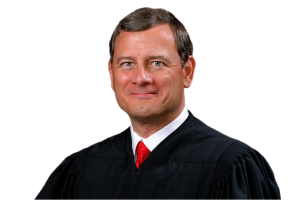
\includegraphics[width=1.5in,height=1.5in]{../../../../data/justice_images/Roberts.png}}}} & \multicolumn{1}{>{\centering\arraybackslash}p{0.75in}}{\textbf{\makebox[0pt][c]{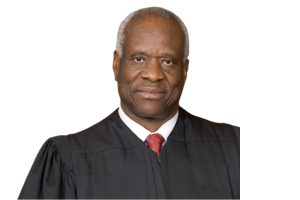
\includegraphics[width=1.5in,height=1.5in]{../../../../data/justice_images/Thomas.png}}}} & \multicolumn{1}{>{\centering\arraybackslash}p{0.75in}}{\textbf{\makebox[0pt][c]{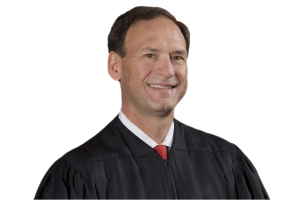
\includegraphics[width=1.5in,height=1.5in]{../../../../data/justice_images/Alito.png}}}} & \multicolumn{1}{>{\centering\arraybackslash}p{0.75in}}{\textbf{\makebox[0pt][c]{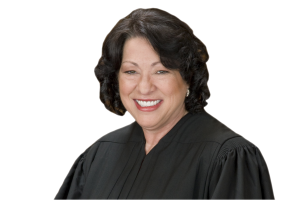
\includegraphics[width=1.5in,height=1.5in]{../../../../data/justice_images/Sotomayor.png}}}} & \multicolumn{1}{>{\centering\arraybackslash}p{0.75in}}{\textbf{\makebox[0pt][c]{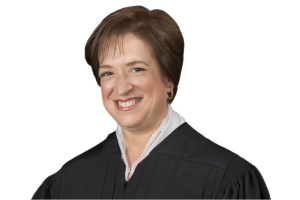
\includegraphics[width=1.5in,height=1.5in]{../../../../data/justice_images/Kagan.png}}}} & \multicolumn{1}{>{\centering\arraybackslash}p{0.75in}}{\textbf{\makebox[0pt][c]{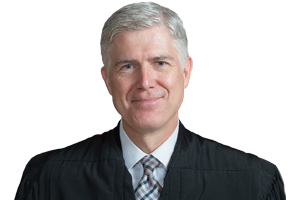
\includegraphics[width=1.5in,height=1.5in]{../../../../data/justice_images/Gorsuch.png}}}} & \multicolumn{1}{>{\centering\arraybackslash}p{0.75in}}{\textbf{\makebox[0pt][c]{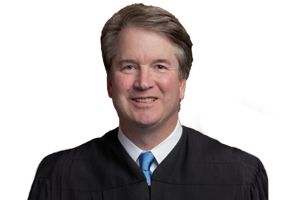
\includegraphics[width=1.5in,height=1.5in]{../../../../data/justice_images/Kavanaugh.png}}}} & \multicolumn{1}{>{\centering\arraybackslash}p{0.75in}}{\textbf{\makebox[0pt][c]{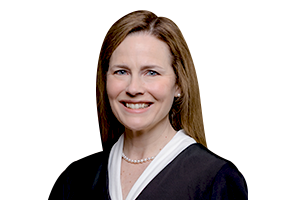
\includegraphics[width=1.5in,height=1.5in]{../../../../data/justice_images/Barrett.png}}}} & \multicolumn{1}{>{\centering\arraybackslash}p{0.75in}}{\textbf{\makebox[0pt][c]{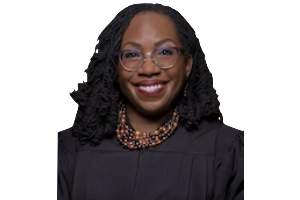
\includegraphics[width=1.5in,height=1.5in]{../../../../data/justice_images/Jackson.png}}}}\\
\addlinespace[0.3em]
\midrule
\endfirsthead
\multicolumn{13}{@{}l}{\textit{(continued)}}\\
\multicolumn{1}{c}{\textbf{Case Name}} & \multicolumn{1}{c}{\textbf{Decided}} & \multicolumn{1}{c}{\textbf{Vote}} & \multicolumn{1}{c}{\textbf{Author}} & \multicolumn{1}{>{\centering\arraybackslash}p{0.75in}}{\textbf{\makebox[0pt][c]{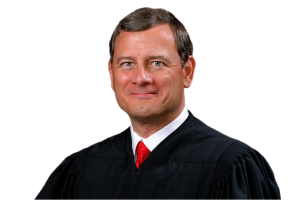
\includegraphics[width=1.5in,height=1.5in]{../../../../data/justice_images/Roberts.png}}}} & \multicolumn{1}{>{\centering\arraybackslash}p{0.75in}}{\textbf{\makebox[0pt][c]{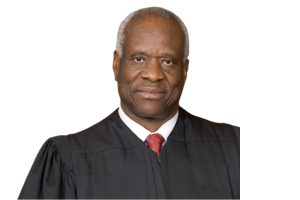
\includegraphics[width=1.5in,height=1.5in]{../../../../data/justice_images/Thomas.png}}}} & \multicolumn{1}{>{\centering\arraybackslash}p{0.75in}}{\textbf{\makebox[0pt][c]{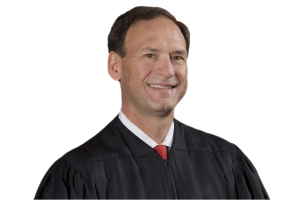
\includegraphics[width=1.5in,height=1.5in]{../../../../data/justice_images/Alito.png}}}} & \multicolumn{1}{>{\centering\arraybackslash}p{0.75in}}{\textbf{\makebox[0pt][c]{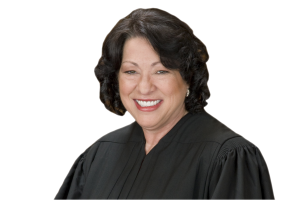
\includegraphics[width=1.5in,height=1.5in]{../../../../data/justice_images/Sotomayor.png}}}} & \multicolumn{1}{>{\centering\arraybackslash}p{0.75in}}{\textbf{\makebox[0pt][c]{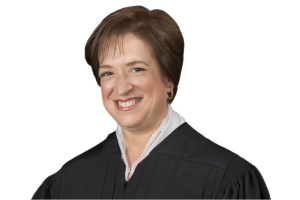
\includegraphics[width=1.5in,height=1.5in]{../../../../data/justice_images/Kagan.png}}}} & \multicolumn{1}{>{\centering\arraybackslash}p{0.75in}}{\textbf{\makebox[0pt][c]{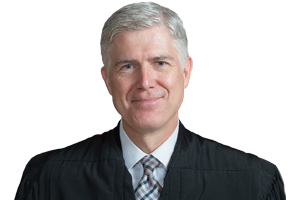
\includegraphics[width=1.5in,height=1.5in]{../../../../data/justice_images/Gorsuch.png}}}} & \multicolumn{1}{>{\centering\arraybackslash}p{0.75in}}{\textbf{\makebox[0pt][c]{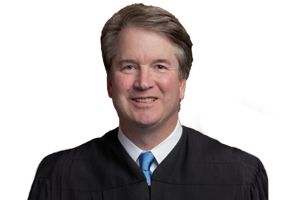
\includegraphics[width=1.5in,height=1.5in]{../../../../data/justice_images/Kavanaugh.png}}}} & \multicolumn{1}{>{\centering\arraybackslash}p{0.75in}}{\textbf{\makebox[0pt][c]{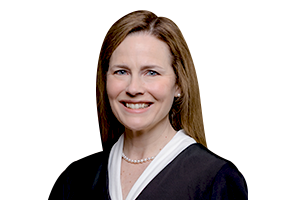
\includegraphics[width=1.5in,height=1.5in]{../../../../data/justice_images/Barrett.png}}}} & \multicolumn{1}{>{\centering\arraybackslash}p{0.75in}}{\textbf{\makebox[0pt][c]{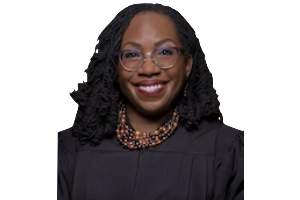
\includegraphics[width=1.5in,height=1.5in]{../../../../data/justice_images/Jackson.png}}}}\\
\addlinespace[0.3em]
\midrule
\endhead

\endfoot
\bottomrule
\endlastfoot
\cellcolor{white}{Clark} & \cellcolor{white}{11/24/2025} & \cellcolor{white}{(9-0)} & \cellcolor{white}{PC} & \cellcolor[HTML]{4f4789}{\textcolor{white}{ }} & \cellcolor[HTML]{4f4789}{\textcolor{white}{ }} & \cellcolor[HTML]{4f4789}{\textcolor{white}{ }} & \cellcolor[HTML]{4f4789}{\textcolor{white}{ }} & \cellcolor[HTML]{4f4789}{\textcolor{white}{ }} & \cellcolor[HTML]{4f4789}{\textcolor{white}{ }} & \cellcolor[HTML]{4f4789}{\textcolor{white}{ }} & \cellcolor[HTML]{4f4789}{\textcolor{white}{ }} & \cellcolor[HTML]{4f4789}{\textcolor{white}{ }}\\
\addlinespace[0.3em]
\cellcolor[HTML]{f7f7f7}{Pitts} & \cellcolor[HTML]{f7f7f7}{11/24/2025} & \cellcolor[HTML]{f7f7f7}{(9-0)} & \cellcolor[HTML]{f7f7f7}{PC} & \cellcolor[HTML]{4f4789}{\textcolor{white}{ }} & \cellcolor[HTML]{4f4789}{\textcolor{white}{ }} & \cellcolor[HTML]{4f4789}{\textcolor{white}{ }} & \cellcolor[HTML]{4f4789}{\textcolor{white}{ }} & \cellcolor[HTML]{4f4789}{\textcolor{white}{ }} & \cellcolor[HTML]{4f4789}{\textcolor{white}{ }} & \cellcolor[HTML]{4f4789}{\textcolor{white}{ }} & \cellcolor[HTML]{4f4789}{\textcolor{white}{ }} & \cellcolor[HTML]{4f4789}{\textcolor{white}{ }}\\
\addlinespace[0.3em]
\cellcolor{white}{Dynamic PT} & \cellcolor{white}{12/8/2025} & \cellcolor{white}{(9-0)} & \cellcolor{white}{PC} & \cellcolor[HTML]{4f4789}{\textcolor{white}{ }} & \cellcolor[HTML]{4f4789}{\textcolor{white}{ }} & \cellcolor[HTML]{4f4789}{\textcolor{white}{ }} & \cellcolor[HTML]{4f4789}{\textcolor{white}{ }} & \cellcolor[HTML]{4f4789}{\textcolor{white}{ }} & \cellcolor[HTML]{4f4789}{\textcolor{white}{ }} & \cellcolor[HTML]{4f4789}{\textcolor{white}{ }} & \cellcolor[HTML]{4f4789}{\textcolor{white}{ }} & \cellcolor[HTML]{4f4789}{\textcolor{white}{ }}\\
\addlinespace[0.3em]
\cellcolor[HTML]{f7f7f7}{Bowe\textsuperscript{(1)}} & \cellcolor[HTML]{f7f7f7}{1/9/2026} & \cellcolor[HTML]{f7f7f7}{(5-4)} & \cellcolor[HTML]{f7f7f7}{Sotomayor} & \cellcolor[HTML]{4f4789}{\textcolor{white}{ }} & \cellcolor[HTML]{ff0000}{\textcolor{white}{ }} & \cellcolor[HTML]{ff0000}{\textcolor{white}{ }} & \cellcolor[HTML]{4f4789}{\textcolor{white}{ }} & \cellcolor[HTML]{4f4789}{\textcolor{white}{ }} & \cellcolor[HTML]{ff0000}{\textcolor{white}{ }} & \cellcolor[HTML]{4f4789}{\textcolor{white}{ }} & \cellcolor[HTML]{ff0000}{\textcolor{white}{ }} & \cellcolor[HTML]{4f4789}{\textcolor{white}{ }}\\
\addlinespace[0.3em]
\cellcolor{white}{Barrett\textsuperscript{(2)}} & \cellcolor{white}{1/14/2026} & \cellcolor{white}{(9-0)} & \cellcolor{white}{Jackson} & \cellcolor[HTML]{4f4789}{\textcolor{white}{ }} & \cellcolor[HTML]{4f4789}{\textcolor{white}{ }} & \cellcolor[HTML]{4f4789}{\textcolor{white}{ }} & \cellcolor[HTML]{4f4789}{\textcolor{white}{ }} & \cellcolor[HTML]{4f4789}{\textcolor{white}{ }} & \cellcolor[HTML]{70ac47}{\textcolor{white}{ }} & \cellcolor[HTML]{4f4789}{\textcolor{white}{ }} & \cellcolor[HTML]{4f4789}{\textcolor{white}{ }} & \cellcolor[HTML]{4f4789}{\textcolor{white}{ }}\\
\addlinespace[0.3em]
\cellcolor[HTML]{f7f7f7}{Bost} & \cellcolor[HTML]{f7f7f7}{1/14/2026} & \cellcolor[HTML]{f7f7f7}{(7-2)} & \cellcolor[HTML]{f7f7f7}{Roberts} & \cellcolor[HTML]{4f4789}{\textcolor{white}{ }} & \cellcolor[HTML]{4f4789}{\textcolor{white}{ }} & \cellcolor[HTML]{4f4789}{\textcolor{white}{ }} & \cellcolor[HTML]{ff0000}{\textcolor{white}{ }} & \cellcolor[HTML]{4f4789}{\textcolor{white}{ }} & \cellcolor[HTML]{4f4789}{\textcolor{white}{ }} & \cellcolor[HTML]{4f4789}{\textcolor{white}{ }} & \cellcolor[HTML]{70ac47}{\textcolor{white}{ }} & \cellcolor[HTML]{ff0000}{\textcolor{white}{ }}\\
\addlinespace[0.3em]
\cellcolor{white}{Case} & \cellcolor{white}{1/14/2026} & \cellcolor{white}{(9-0)} & \cellcolor{white}{Kagan} & \cellcolor[HTML]{4f4789}{\textcolor{white}{ }} & \cellcolor[HTML]{4f4789}{\textcolor{white}{ }} & \cellcolor[HTML]{4f4789}{\textcolor{white}{ }} & \cellcolor[HTML]{4f4789}{\textcolor{white}{ }} & \cellcolor[HTML]{4f4789}{\textcolor{white}{ }} & \cellcolor[HTML]{4f4789}{\textcolor{white}{ }} & \cellcolor[HTML]{4f4789}{\textcolor{white}{ }} & \cellcolor[HTML]{4f4789}{\textcolor{white}{ }} & \cellcolor[HTML]{4f4789}{\textcolor{white}{ }}\\
\addlinespace[0.3em]
\cellcolor[HTML]{f7f7f7}{Berk} & \cellcolor[HTML]{f7f7f7}{1/20/2026} & \cellcolor[HTML]{f7f7f7}{(9-0)} & \cellcolor[HTML]{f7f7f7}{Barrett} & \cellcolor[HTML]{4f4789}{\textcolor{white}{ }} & \cellcolor[HTML]{4f4789}{\textcolor{white}{ }} & \cellcolor[HTML]{4f4789}{\textcolor{white}{ }} & \cellcolor[HTML]{4f4789}{\textcolor{white}{ }} & \cellcolor[HTML]{4f4789}{\textcolor{white}{ }} & \cellcolor[HTML]{4f4789}{\textcolor{white}{ }} & \cellcolor[HTML]{4f4789}{\textcolor{white}{ }} & \cellcolor[HTML]{4f4789}{\textcolor{white}{ }} & \cellcolor[HTML]{70ac47}{\textcolor{white}{ }}\\
\addlinespace[0.3em]
\cellcolor{white}{Coney Island Auto} & \cellcolor{white}{1/20/2026} & \cellcolor{white}{(9-0)} & \cellcolor{white}{Alito} & \cellcolor[HTML]{4f4789}{\textcolor{white}{ }} & \cellcolor[HTML]{4f4789}{\textcolor{white}{ }} & \cellcolor[HTML]{4f4789}{\textcolor{white}{ }} & \cellcolor[HTML]{70ac47}{\textcolor{white}{ }} & \cellcolor[HTML]{4f4789}{\textcolor{white}{ }} & \cellcolor[HTML]{4f4789}{\textcolor{white}{ }} & \cellcolor[HTML]{4f4789}{\textcolor{white}{ }} & \cellcolor[HTML]{4f4789}{\textcolor{white}{ }} & \cellcolor[HTML]{4f4789}{\textcolor{white}{ }}\\
\addlinespace[0.3em]
\cellcolor[HTML]{f7f7f7}{Ellingburg} & \cellcolor[HTML]{f7f7f7}{1/20/2026} & \cellcolor[HTML]{f7f7f7}{(9-0)} & \cellcolor[HTML]{f7f7f7}{Kavanaugh} & \cellcolor[HTML]{4f4789}{\textcolor{white}{ }} & \cellcolor[HTML]{4f4789}{\textcolor{white}{ }} & \cellcolor[HTML]{4f4789}{\textcolor{white}{ }} & \cellcolor[HTML]{4f4789}{\textcolor{white}{ }} & \cellcolor[HTML]{4f4789}{\textcolor{white}{ }} & \cellcolor[HTML]{4f4789}{\textcolor{white}{ }} & \cellcolor[HTML]{4f4789}{\textcolor{white}{ }} & \cellcolor[HTML]{4f4789}{\textcolor{white}{ }} & \cellcolor[HTML]{4f4789}{\textcolor{white}{ }}\\
\addlinespace[0.3em]
\cellcolor{white}{Klein\textsuperscript{(3)}} & \cellcolor{white}{1/26/2026} & \cellcolor{white}{(8-1)} & \cellcolor{white}{PC} & \cellcolor[HTML]{4f4789}{\textcolor{white}{ }} & \cellcolor[HTML]{4f4789}{\textcolor{white}{ }} & \cellcolor[HTML]{4f4789}{\textcolor{white}{ }} & \cellcolor[HTML]{4f4789}{\textcolor{white}{ }} & \cellcolor[HTML]{4f4789}{\textcolor{white}{ }} & \cellcolor[HTML]{4f4789}{\textcolor{white}{ }} & \cellcolor[HTML]{4f4789}{\textcolor{white}{ }} & \cellcolor[HTML]{4f4789}{\textcolor{white}{ }} & \cellcolor[HTML]{ff0000}{\textcolor{white}{ }}\\
\addlinespace[0.3em]
\cellcolor[HTML]{f7f7f7}{Learning Resources\textsuperscript{(4)}} & \cellcolor[HTML]{f7f7f7}{2/20/2026} & \cellcolor[HTML]{f7f7f7}{(6-3)} & \cellcolor[HTML]{f7f7f7}{Roberts} & \cellcolor[HTML]{4f4789}{\textcolor{white}{ }} & \cellcolor[HTML]{ff0000}{\textcolor{white}{ }} & \cellcolor[HTML]{ff0000}{\textcolor{white}{ }} & \cellcolor[HTML]{4f4789}{\textcolor{white}{ }} & \cellcolor[HTML]{70ac47}{\textcolor{white}{ }} & \cellcolor[HTML]{4f4789}{\textcolor{white}{ }} & \cellcolor[HTML]{ff0000}{\textcolor{white}{ }} & \cellcolor[HTML]{4f4789}{\textcolor{white}{ }} & \cellcolor[HTML]{70ac47}{\textcolor{white}{ }}\\
\addlinespace[0.3em]
\cellcolor{white}{Hain Celestial Grp.} & \cellcolor{white}{2/24/2026} & \cellcolor{white}{(9-0)} & \cellcolor{white}{Sotomayor} & \cellcolor[HTML]{4f4789}{\textcolor{white}{ }} & \cellcolor[HTML]{4f4789}{\textcolor{white}{ }} & \cellcolor[HTML]{4f4789}{\textcolor{white}{ }} & \cellcolor[HTML]{4f4789}{\textcolor{white}{ }} & \cellcolor[HTML]{4f4789}{\textcolor{white}{ }} & \cellcolor[HTML]{4f4789}{\textcolor{white}{ }} & \cellcolor[HTML]{4f4789}{\textcolor{white}{ }} & \cellcolor[HTML]{4f4789}{\textcolor{white}{ }} & \cellcolor[HTML]{4f4789}{\textcolor{white}{ }}\\
\addlinespace[0.3em]
\cellcolor[HTML]{f7f7f7}{USPS} & \cellcolor[HTML]{f7f7f7}{2/24/2026} & \cellcolor[HTML]{f7f7f7}{(5-4)} & \cellcolor[HTML]{f7f7f7}{Thomas} & \cellcolor[HTML]{4f4789}{\textcolor{white}{ }} & \cellcolor[HTML]{4f4789}{\textcolor{white}{ }} & \cellcolor[HTML]{4f4789}{\textcolor{white}{ }} & \cellcolor[HTML]{ff0000}{\textcolor{white}{ }} & \cellcolor[HTML]{ff0000}{\textcolor{white}{ }} & \cellcolor[HTML]{ff0000}{\textcolor{white}{ }} & \cellcolor[HTML]{4f4789}{\textcolor{white}{ }} & \cellcolor[HTML]{4f4789}{\textcolor{white}{ }} & \cellcolor[HTML]{ff0000}{\textcolor{white}{ }}\\
\addlinespace[0.3em]
\cellcolor{white}{GEO Group} & \cellcolor{white}{2/25/2026} & \cellcolor{white}{(9-0)} & \cellcolor{white}{Kagan} & \cellcolor[HTML]{4f4789}{\textcolor{white}{ }} & \cellcolor[HTML]{70ac47}{\textcolor{white}{ }} & \cellcolor[HTML]{70ac47}{\textcolor{white}{ }} & \cellcolor[HTML]{4f4789}{\textcolor{white}{ }} & \cellcolor[HTML]{4f4789}{\textcolor{white}{ }} & \cellcolor[HTML]{4f4789}{\textcolor{white}{ }} & \cellcolor[HTML]{4f4789}{\textcolor{white}{ }} & \cellcolor[HTML]{4f4789}{\textcolor{white}{ }} & \cellcolor[HTML]{4f4789}{\textcolor{white}{ }}\\
\addlinespace[0.3em]
\cellcolor[HTML]{f7f7f7}{Villarreal} & \cellcolor[HTML]{f7f7f7}{2/25/2026} & \cellcolor[HTML]{f7f7f7}{(9-0)} & \cellcolor[HTML]{f7f7f7}{Jackson} & \cellcolor[HTML]{4f4789}{\textcolor{white}{ }} & \cellcolor[HTML]{70ac47}{\textcolor{white}{ }} & \cellcolor[HTML]{4f4789}{\textcolor{white}{ }} & \cellcolor[HTML]{4f4789}{\textcolor{white}{ }} & \cellcolor[HTML]{4f4789}{\textcolor{white}{ }} & \cellcolor[HTML]{4f4789}{\textcolor{white}{ }} & \cellcolor[HTML]{4f4789}{\textcolor{white}{ }} & \cellcolor[HTML]{4f4789}{\textcolor{white}{ }} & \cellcolor[HTML]{4f4789}{\textcolor{white}{ }}\\
\addlinespace[0.3em]
\cellcolor{white}{Galette} & \cellcolor{white}{3/4/2026} & \cellcolor{white}{(9-0)} & \cellcolor{white}{Sotomayor} & \cellcolor[HTML]{4f4789}{\textcolor{white}{ }} & \cellcolor[HTML]{4f4789}{\textcolor{white}{ }} & \cellcolor[HTML]{4f4789}{\textcolor{white}{ }} & \cellcolor[HTML]{4f4789}{\textcolor{white}{ }} & \cellcolor[HTML]{4f4789}{\textcolor{white}{ }} & \cellcolor[HTML]{4f4789}{\textcolor{white}{ }} & \cellcolor[HTML]{4f4789}{\textcolor{white}{ }} & \cellcolor[HTML]{4f4789}{\textcolor{white}{ }} & \cellcolor[HTML]{4f4789}{\textcolor{white}{ }}\\
\addlinespace[0.3em]
\cellcolor[HTML]{f7f7f7}{Urias-Orellana} & \cellcolor[HTML]{f7f7f7}{3/4/2026} & \cellcolor[HTML]{f7f7f7}{(9-0)} & \cellcolor[HTML]{f7f7f7}{Jackson} & \cellcolor[HTML]{4f4789}{\textcolor{white}{ }} & \cellcolor[HTML]{4f4789}{\textcolor{white}{ }} & \cellcolor[HTML]{4f4789}{\textcolor{white}{ }} & \cellcolor[HTML]{4f4789}{\textcolor{white}{ }} & \cellcolor[HTML]{4f4789}{\textcolor{white}{ }} & \cellcolor[HTML]{4f4789}{\textcolor{white}{ }} & \cellcolor[HTML]{4f4789}{\textcolor{white}{ }} & \cellcolor[HTML]{4f4789}{\textcolor{white}{ }} & \cellcolor[HTML]{4f4789}{\textcolor{white}{ }}\\
\addlinespace[0.3em]
\cellcolor{white}{Olivier} & \cellcolor{white}{3/20/2026} & \cellcolor{white}{(9-0)} & \cellcolor{white}{Kagan} & \cellcolor[HTML]{4f4789}{\textcolor{white}{ }} & \cellcolor[HTML]{4f4789}{\textcolor{white}{ }} & \cellcolor[HTML]{4f4789}{\textcolor{white}{ }} & \cellcolor[HTML]{4f4789}{\textcolor{white}{ }} & \cellcolor[HTML]{4f4789}{\textcolor{white}{ }} & \cellcolor[HTML]{4f4789}{\textcolor{white}{ }} & \cellcolor[HTML]{4f4789}{\textcolor{white}{ }} & \cellcolor[HTML]{4f4789}{\textcolor{white}{ }} & \cellcolor[HTML]{4f4789}{\textcolor{white}{ }}\\
\addlinespace[0.3em]
\cellcolor[HTML]{f7f7f7}{Zorn} & \cellcolor[HTML]{f7f7f7}{3/23/2026} & \cellcolor[HTML]{f7f7f7}{(6-3)} & \cellcolor[HTML]{f7f7f7}{PC} & \cellcolor[HTML]{4f4789}{\textcolor{white}{ }} & \cellcolor[HTML]{4f4789}{\textcolor{white}{ }} & \cellcolor[HTML]{4f4789}{\textcolor{white}{ }} & \cellcolor[HTML]{ff0000}{\textcolor{white}{ }} & \cellcolor[HTML]{ff0000}{\textcolor{white}{ }} & \cellcolor[HTML]{4f4789}{\textcolor{white}{ }} & \cellcolor[HTML]{4f4789}{\textcolor{white}{ }} & \cellcolor[HTML]{4f4789}{\textcolor{white}{ }} & \cellcolor[HTML]{ff0000}{\textcolor{white}{ }}\\
\addlinespace[0.3em]
\cellcolor{white}{Cox} & \cellcolor{white}{3/25/2026} & \cellcolor{white}{(9-0)} & \cellcolor{white}{Thomas} & \cellcolor[HTML]{4f4789}{\textcolor{white}{ }} & \cellcolor[HTML]{4f4789}{\textcolor{white}{ }} & \cellcolor[HTML]{4f4789}{\textcolor{white}{ }} & \cellcolor[HTML]{70ac47}{\textcolor{white}{ }} & \cellcolor[HTML]{4f4789}{\textcolor{white}{ }} & \cellcolor[HTML]{4f4789}{\textcolor{white}{ }} & \cellcolor[HTML]{4f4789}{\textcolor{white}{ }} & \cellcolor[HTML]{4f4789}{\textcolor{white}{ }} & \cellcolor[HTML]{4f4789}{\textcolor{white}{ }}\\
\addlinespace[0.3em]
\cellcolor[HTML]{f7f7f7}{Rico} & \cellcolor[HTML]{f7f7f7}{3/25/2026} & \cellcolor[HTML]{f7f7f7}{(8-1)} & \cellcolor[HTML]{f7f7f7}{Gorsuch} & \cellcolor[HTML]{4f4789}{\textcolor{white}{ }} & \cellcolor[HTML]{4f4789}{\textcolor{white}{ }} & \cellcolor[HTML]{ff0000}{\textcolor{white}{ }} & \cellcolor[HTML]{4f4789}{\textcolor{white}{ }} & \cellcolor[HTML]{4f4789}{\textcolor{white}{ }} & \cellcolor[HTML]{4f4789}{\textcolor{white}{ }} & \cellcolor[HTML]{4f4789}{\textcolor{white}{ }} & \cellcolor[HTML]{4f4789}{\textcolor{white}{ }} & \cellcolor[HTML]{4f4789}{\textcolor{white}{ }}\\
\addlinespace[0.3em]
\cellcolor{white}{Chiles} & \cellcolor{white}{3/31/2026} & \cellcolor{white}{(8-1)} & \cellcolor{white}{Gorsuch} & \cellcolor[HTML]{4f4789}{\textcolor{white}{ }} & \cellcolor[HTML]{4f4789}{\textcolor{white}{ }} & \cellcolor[HTML]{4f4789}{\textcolor{white}{ }} & \cellcolor[HTML]{4f4789}{\textcolor{white}{ }} & \cellcolor[HTML]{4f4789}{\textcolor{white}{ }} & \cellcolor[HTML]{4f4789}{\textcolor{white}{ }} & \cellcolor[HTML]{4f4789}{\textcolor{white}{ }} & \cellcolor[HTML]{4f4789}{\textcolor{white}{ }} & \cellcolor[HTML]{ff0000}{\textcolor{white}{ }}\\
\addlinespace[0.3em]
\cellcolor[HTML]{f7f7f7}{Plaquemines Parish} & \cellcolor[HTML]{f7f7f7}{4/17/2026} & \cellcolor[HTML]{f7f7f7}{(8-0)} & \cellcolor[HTML]{f7f7f7}{Thomas} & \cellcolor[HTML]{4f4789}{\textcolor{white}{ }} & \cellcolor[HTML]{4f4789}{\textcolor{white}{ }} & \cellcolor{white}{\textcolor{white}{ }} & \cellcolor[HTML]{4f4789}{\textcolor{white}{ }} & \cellcolor[HTML]{4f4789}{\textcolor{white}{ }} & \cellcolor[HTML]{4f4789}{\textcolor{white}{ }} & \cellcolor[HTML]{4f4789}{\textcolor{white}{ }} & \cellcolor[HTML]{4f4789}{\textcolor{white}{ }} & \cellcolor[HTML]{70ac47}{\textcolor{white}{ }}\\
\addlinespace[0.3em]
\cellcolor{white}{R.W.\textsuperscript{(5)}} & \cellcolor{white}{4/20/2026} & \cellcolor{white}{(7-2)} & \cellcolor{white}{PC} & \cellcolor[HTML]{4f4789}{\textcolor{white}{ }} & \cellcolor[HTML]{4f4789}{\textcolor{white}{ }} & \cellcolor[HTML]{4f4789}{\textcolor{white}{ }} & \cellcolor[HTML]{ff0000}{\textcolor{white}{ }} & \cellcolor[HTML]{4f4789}{\textcolor{white}{ }} & \cellcolor[HTML]{4f4789}{\textcolor{white}{ }} & \cellcolor[HTML]{4f4789}{\textcolor{white}{ }} & \cellcolor[HTML]{4f4789}{\textcolor{white}{ }} & \cellcolor[HTML]{ff0000}{\textcolor{white}{ }}\\
\addlinespace[0.3em]
\cellcolor[HTML]{f7f7f7}{Enbridge} & \cellcolor[HTML]{f7f7f7}{4/22/2026} & \cellcolor[HTML]{f7f7f7}{(9-0)} & \cellcolor[HTML]{f7f7f7}{Sotomayor} & \cellcolor[HTML]{4f4789}{\textcolor{white}{ }} & \cellcolor[HTML]{4f4789}{\textcolor{white}{ }} & \cellcolor[HTML]{4f4789}{\textcolor{white}{ }} & \cellcolor[HTML]{4f4789}{\textcolor{white}{ }} & \cellcolor[HTML]{4f4789}{\textcolor{white}{ }} & \cellcolor[HTML]{4f4789}{\textcolor{white}{ }} & \cellcolor[HTML]{4f4789}{\textcolor{white}{ }} & \cellcolor[HTML]{4f4789}{\textcolor{white}{ }} & \cellcolor[HTML]{4f4789}{\textcolor{white}{ }}\\
\addlinespace[0.3em]
\cellcolor{white}{Hencely} & \cellcolor{white}{4/22/2026} & \cellcolor{white}{(6-3)} & \cellcolor{white}{Thomas} & \cellcolor[HTML]{ff0000}{\textcolor{white}{ }} & \cellcolor[HTML]{4f4789}{\textcolor{white}{ }} & \cellcolor[HTML]{ff0000}{\textcolor{white}{ }} & \cellcolor[HTML]{4f4789}{\textcolor{white}{ }} & \cellcolor[HTML]{4f4789}{\textcolor{white}{ }} & \cellcolor[HTML]{4f4789}{\textcolor{white}{ }} & \cellcolor[HTML]{ff0000}{\textcolor{white}{ }} & \cellcolor[HTML]{4f4789}{\textcolor{white}{ }} & \cellcolor[HTML]{4f4789}{\textcolor{white}{ }}\\
\addlinespace[0.3em]
\cellcolor[HTML]{f7f7f7}{First Choice} & \cellcolor[HTML]{f7f7f7}{4/29/2026} & \cellcolor[HTML]{f7f7f7}{(9-0)} & \cellcolor[HTML]{f7f7f7}{Gorsuch} & \cellcolor[HTML]{4f4789}{\textcolor{white}{ }} & \cellcolor[HTML]{4f4789}{\textcolor{white}{ }} & \cellcolor[HTML]{4f4789}{\textcolor{white}{ }} & \cellcolor[HTML]{4f4789}{\textcolor{white}{ }} & \cellcolor[HTML]{4f4789}{\textcolor{white}{ }} & \cellcolor[HTML]{4f4789}{\textcolor{white}{ }} & \cellcolor[HTML]{4f4789}{\textcolor{white}{ }} & \cellcolor[HTML]{4f4789}{\textcolor{white}{ }} & \cellcolor[HTML]{4f4789}{\textcolor{white}{ }}\\
\addlinespace[0.3em]
\cellcolor{white}{Callais} & \cellcolor{white}{4/29/2026} & \cellcolor{white}{(6-3)} & \cellcolor{white}{Alito} & \cellcolor[HTML]{4f4789}{\textcolor{white}{ }} & \cellcolor[HTML]{4f4789}{\textcolor{white}{ }} & \cellcolor[HTML]{4f4789}{\textcolor{white}{ }} & \cellcolor[HTML]{ff0000}{\textcolor{white}{ }} & \cellcolor[HTML]{ff0000}{\textcolor{white}{ }} & \cellcolor[HTML]{4f4789}{\textcolor{white}{ }} & \cellcolor[HTML]{4f4789}{\textcolor{white}{ }} & \cellcolor[HTML]{4f4789}{\textcolor{white}{ }} & \cellcolor[HTML]{ff0000}{\textcolor{white}{ }}\\
\addlinespace[0.3em]
\cellcolor[HTML]{f7f7f7}{Jules} & \cellcolor[HTML]{f7f7f7}{5/14/2026} & \cellcolor[HTML]{f7f7f7}{(9-0)} & \cellcolor[HTML]{f7f7f7}{Sotomayor} & \cellcolor[HTML]{4f4789}{\textcolor{white}{ }} & \cellcolor[HTML]{4f4789}{\textcolor{white}{ }} & \cellcolor[HTML]{4f4789}{\textcolor{white}{ }} & \cellcolor[HTML]{4f4789}{\textcolor{white}{ }} & \cellcolor[HTML]{4f4789}{\textcolor{white}{ }} & \cellcolor[HTML]{4f4789}{\textcolor{white}{ }} & \cellcolor[HTML]{4f4789}{\textcolor{white}{ }} & \cellcolor[HTML]{4f4789}{\textcolor{white}{ }} & \cellcolor[HTML]{4f4789}{\textcolor{white}{ }}\\
\addlinespace[0.3em]
\cellcolor{white}{Montgomery} & \cellcolor{white}{5/14/2026} & \cellcolor{white}{(9-0)} & \cellcolor{white}{Barrett} & \cellcolor[HTML]{4f4789}{\textcolor{white}{ }} & \cellcolor[HTML]{4f4789}{\textcolor{white}{ }} & \cellcolor[HTML]{4f4789}{\textcolor{white}{ }} & \cellcolor[HTML]{4f4789}{\textcolor{white}{ }} & \cellcolor[HTML]{4f4789}{\textcolor{white}{ }} & \cellcolor[HTML]{4f4789}{\textcolor{white}{ }} & \cellcolor[HTML]{4f4789}{\textcolor{white}{ }} & \cellcolor[HTML]{4f4789}{\textcolor{white}{ }} & \cellcolor[HTML]{4f4789}{\textcolor{white}{ }}\\
\addlinespace[0.3em]
\cellcolor[HTML]{f7f7f7}{Havana Docks} & \cellcolor[HTML]{f7f7f7}{5/21/2026} & \cellcolor[HTML]{f7f7f7}{(8-1)} & \cellcolor[HTML]{f7f7f7}{Thomas} & \cellcolor[HTML]{4f4789}{\textcolor{white}{ }} & \cellcolor[HTML]{4f4789}{\textcolor{white}{ }} & \cellcolor[HTML]{4f4789}{\textcolor{white}{ }} & \cellcolor[HTML]{4f4789}{\textcolor{white}{ }} & \cellcolor[HTML]{ff0000}{\textcolor{white}{ }} & \cellcolor[HTML]{4f4789}{\textcolor{white}{ }} & \cellcolor[HTML]{4f4789}{\textcolor{white}{ }} & \cellcolor[HTML]{4f4789}{\textcolor{white}{ }} & \cellcolor[HTML]{4f4789}{\textcolor{white}{ }}\\
\addlinespace[0.3em]
\cellcolor{white}{IAM Pension Fund} & \cellcolor{white}{5/21/2026} & \cellcolor{white}{(9-0)} & \cellcolor{white}{Jackson} & \cellcolor[HTML]{4f4789}{\textcolor{white}{ }} & \cellcolor[HTML]{4f4789}{\textcolor{white}{ }} & \cellcolor[HTML]{4f4789}{\textcolor{white}{ }} & \cellcolor[HTML]{4f4789}{\textcolor{white}{ }} & \cellcolor[HTML]{4f4789}{\textcolor{white}{ }} & \cellcolor[HTML]{4f4789}{\textcolor{white}{ }} & \cellcolor[HTML]{4f4789}{\textcolor{white}{ }} & \cellcolor[HTML]{4f4789}{\textcolor{white}{ }} & \cellcolor[HTML]{4f4789}{\textcolor{white}{ }}\\
\addlinespace[0.3em]
\cellcolor[HTML]{f7f7f7}{Hamm\textsuperscript{(6)}} & \cellcolor[HTML]{f7f7f7}{5/21/2026} & \cellcolor[HTML]{f7f7f7}{(5-4)} & \cellcolor[HTML]{f7f7f7}{PC} & \cellcolor[HTML]{ff0000}{\textcolor{white}{ }} & \cellcolor[HTML]{ff0000}{\textcolor{white}{ }} & \cellcolor[HTML]{ff0000}{\textcolor{white}{ }} & \cellcolor[HTML]{4f4789}{\textcolor{white}{ }} & \cellcolor[HTML]{4f4789}{\textcolor{white}{ }} & \cellcolor[HTML]{ff0000}{\textcolor{white}{ }} & \cellcolor[HTML]{4f4789}{\textcolor{white}{ }} & \cellcolor[HTML]{4f4789}{\textcolor{white}{ }} & \cellcolor[HTML]{4f4789}{\textcolor{white}{ }}\\
\addlinespace[0.3em]
\cellcolor{white}{Margolin} & \cellcolor{white}{5/26/2026} & \cellcolor{white}{(9-0)} & \cellcolor{white}{PC} & \cellcolor[HTML]{4f4789}{\textcolor{white}{ }} & \cellcolor[HTML]{4f4789}{\textcolor{white}{ }} & \cellcolor[HTML]{4f4789}{\textcolor{white}{ }} & \cellcolor[HTML]{4f4789}{\textcolor{white}{ }} & \cellcolor[HTML]{4f4789}{\textcolor{white}{ }} & \cellcolor[HTML]{4f4789}{\textcolor{white}{ }} & \cellcolor[HTML]{4f4789}{\textcolor{white}{ }} & \cellcolor[HTML]{4f4789}{\textcolor{white}{ }} & \cellcolor[HTML]{4f4789}{\textcolor{white}{ }}\\
\addlinespace[0.3em]
\cellcolor[HTML]{f7f7f7}{Flowers Foods} & \cellcolor[HTML]{f7f7f7}{5/28/2026} & \cellcolor[HTML]{f7f7f7}{(9-0)} & \cellcolor[HTML]{f7f7f7}{Gorsuch} & \cellcolor[HTML]{4f4789}{\textcolor{white}{ }} & \cellcolor[HTML]{4f4789}{\textcolor{white}{ }} & \cellcolor[HTML]{4f4789}{\textcolor{white}{ }} & \cellcolor[HTML]{4f4789}{\textcolor{white}{ }} & \cellcolor[HTML]{4f4789}{\textcolor{white}{ }} & \cellcolor[HTML]{4f4789}{\textcolor{white}{ }} & \cellcolor[HTML]{4f4789}{\textcolor{white}{ }} & \cellcolor[HTML]{4f4789}{\textcolor{white}{ }} & \cellcolor[HTML]{4f4789}{\textcolor{white}{ }}\\
\addlinespace[0.3em]
\cellcolor{white}{Pitchford} & \cellcolor{white}{5/28/2026} & \cellcolor{white}{(5-4)} & \cellcolor{white}{Kavanaugh} & \cellcolor[HTML]{4f4789}{\textcolor{white}{ }} & \cellcolor[HTML]{ff0000}{\textcolor{white}{ }} & \cellcolor[HTML]{ff0000}{\textcolor{white}{ }} & \cellcolor[HTML]{4f4789}{\textcolor{white}{ }} & \cellcolor[HTML]{4f4789}{\textcolor{white}{ }} & \cellcolor[HTML]{ff0000}{\textcolor{white}{ }} & \cellcolor[HTML]{4f4789}{\textcolor{white}{ }} & \cellcolor[HTML]{ff0000}{\textcolor{white}{ }} & \cellcolor[HTML]{4f4789}{\textcolor{white}{ }}\\
\addlinespace[0.3em]
\cellcolor[HTML]{f7f7f7}{Fernandez} & \cellcolor[HTML]{f7f7f7}{5/28/2026} & \cellcolor[HTML]{f7f7f7}{(8-1)} & \cellcolor[HTML]{f7f7f7}{Barrett} & \cellcolor[HTML]{4f4789}{\textcolor{white}{ }} & \cellcolor[HTML]{4f4789}{\textcolor{white}{ }} & \cellcolor[HTML]{4f4789}{\textcolor{white}{ }} & \cellcolor[HTML]{70ac47}{\textcolor{white}{ }} & \cellcolor[HTML]{4f4789}{\textcolor{white}{ }} & \cellcolor[HTML]{4f4789}{\textcolor{white}{ }} & \cellcolor[HTML]{4f4789}{\textcolor{white}{ }} & \cellcolor[HTML]{4f4789}{\textcolor{white}{ }} & \cellcolor[HTML]{ff0000}{\textcolor{white}{ }}\\
\addlinespace[0.3em]
\cellcolor{white}{Rutherford} & \cellcolor{white}{5/28/2026} & \cellcolor{white}{(6-3)} & \cellcolor{white}{Barrett} & \cellcolor[HTML]{4f4789}{\textcolor{white}{ }} & \cellcolor[HTML]{4f4789}{\textcolor{white}{ }} & \cellcolor[HTML]{4f4789}{\textcolor{white}{ }} & \cellcolor[HTML]{ff0000}{\textcolor{white}{ }} & \cellcolor[HTML]{ff0000}{\textcolor{white}{ }} & \cellcolor[HTML]{4f4789}{\textcolor{white}{ }} & \cellcolor[HTML]{4f4789}{\textcolor{white}{ }} & \cellcolor[HTML]{4f4789}{\textcolor{white}{ }} & \cellcolor[HTML]{ff0000}{\textcolor{white}{ }}\\
\addlinespace[0.3em]
\cellcolor[HTML]{f7f7f7}{Whitton\textsuperscript{(7)}} & \cellcolor[HTML]{f7f7f7}{6/1/2026} & \cellcolor[HTML]{f7f7f7}{(7-2)} & \cellcolor[HTML]{f7f7f7}{PC} & \cellcolor[HTML]{4f4789}{\textcolor{white}{ }} & \cellcolor[HTML]{ff0000}{\textcolor{white}{ }} & \cellcolor[HTML]{ff0000}{\textcolor{white}{ }} & \cellcolor[HTML]{4f4789}{\textcolor{white}{ }} & \cellcolor[HTML]{4f4789}{\textcolor{white}{ }} & \cellcolor[HTML]{4f4789}{\textcolor{white}{ }} & \cellcolor[HTML]{4f4789}{\textcolor{white}{ }} & \cellcolor[HTML]{4f4789}{\textcolor{white}{ }} & \cellcolor[HTML]{4f4789}{\textcolor{white}{ }}\\
\addlinespace[0.3em]
\cellcolor{white}{AT\&T} & \cellcolor{white}{6/4/2026} & \cellcolor{white}{(8-1)} & \cellcolor{white}{Roberts} & \cellcolor[HTML]{4f4789}{\textcolor{white}{ }} & \cellcolor[HTML]{ff0000}{\textcolor{white}{ }} & \cellcolor[HTML]{4f4789}{\textcolor{white}{ }} & \cellcolor[HTML]{4f4789}{\textcolor{white}{ }} & \cellcolor[HTML]{4f4789}{\textcolor{white}{ }} & \cellcolor[HTML]{4f4789}{\textcolor{white}{ }} & \cellcolor[HTML]{4f4789}{\textcolor{white}{ }} & \cellcolor[HTML]{4f4789}{\textcolor{white}{ }} & \cellcolor[HTML]{4f4789}{\textcolor{white}{ }}\\
\addlinespace[0.3em]
\cellcolor[HTML]{f7f7f7}{Sripetch} & \cellcolor[HTML]{f7f7f7}{6/4/2026} & \cellcolor[HTML]{f7f7f7}{(9-0)} & \cellcolor[HTML]{f7f7f7}{Gorsuch} & \cellcolor[HTML]{4f4789}{\textcolor{white}{ }} & \cellcolor[HTML]{4f4789}{\textcolor{white}{ }} & \cellcolor[HTML]{4f4789}{\textcolor{white}{ }} & \cellcolor[HTML]{4f4789}{\textcolor{white}{ }} & \cellcolor[HTML]{4f4789}{\textcolor{white}{ }} & \cellcolor[HTML]{4f4789}{\textcolor{white}{ }} & \cellcolor[HTML]{4f4789}{\textcolor{white}{ }} & \cellcolor[HTML]{4f4789}{\textcolor{white}{ }} & \cellcolor[HTML]{4f4789}{\textcolor{white}{ }}\\
\addlinespace[0.3em]
\cellcolor{white}{Hikma} & \cellcolor{white}{6/4/2026} & \cellcolor{white}{(9-0)} & \cellcolor{white}{Jackson} & \cellcolor[HTML]{4f4789}{\textcolor{white}{ }} & \cellcolor[HTML]{4f4789}{\textcolor{white}{ }} & \cellcolor[HTML]{4f4789}{\textcolor{white}{ }} & \cellcolor[HTML]{4f4789}{\textcolor{white}{ }} & \cellcolor[HTML]{4f4789}{\textcolor{white}{ }} & \cellcolor[HTML]{4f4789}{\textcolor{white}{ }} & \cellcolor[HTML]{4f4789}{\textcolor{white}{ }} & \cellcolor[HTML]{4f4789}{\textcolor{white}{ }} & \cellcolor[HTML]{4f4789}{\textcolor{white}{ }}\\
\addlinespace[0.3em]
\cellcolor[HTML]{f7f7f7}{Abouammo} & \cellcolor[HTML]{f7f7f7}{6/11/2026} & \cellcolor[HTML]{f7f7f7}{(9-0)} & \cellcolor[HTML]{f7f7f7}{Kagan} & \cellcolor[HTML]{4f4789}{\textcolor{white}{ }} & \cellcolor[HTML]{4f4789}{\textcolor{white}{ }} & \cellcolor[HTML]{4f4789}{\textcolor{white}{ }} & \cellcolor[HTML]{4f4789}{\textcolor{white}{ }} & \cellcolor[HTML]{4f4789}{\textcolor{white}{ }} & \cellcolor[HTML]{4f4789}{\textcolor{white}{ }} & \cellcolor[HTML]{4f4789}{\textcolor{white}{ }} & \cellcolor[HTML]{4f4789}{\textcolor{white}{ }} & \cellcolor[HTML]{4f4789}{\textcolor{white}{ }}\\
\addlinespace[0.3em]
\cellcolor{white}{FS Credit\textsuperscript{(8)}} & \cellcolor{white}{6/11/2026} & \cellcolor{white}{(6-3)} & \cellcolor{white}{Barrett} & \cellcolor[HTML]{4f4789}{\textcolor{white}{ }} & \cellcolor[HTML]{4f4789}{\textcolor{white}{ }} & \cellcolor[HTML]{4f4789}{\textcolor{white}{ }} & \cellcolor[HTML]{ff0000}{\textcolor{white}{ }} & \cellcolor[HTML]{ff0000}{\textcolor{white}{ }} & \cellcolor[HTML]{4f4789}{\textcolor{white}{ }} & \cellcolor[HTML]{4f4789}{\textcolor{white}{ }} & \cellcolor[HTML]{4f4789}{\textcolor{white}{ }} & \cellcolor[HTML]{ff0000}{\textcolor{white}{ }}\\
\addlinespace[0.3em]
\cellcolor[HTML]{f7f7f7}{Keathley} & \cellcolor[HTML]{f7f7f7}{6/11/2026} & \cellcolor[HTML]{f7f7f7}{(9-0)} & \cellcolor[HTML]{f7f7f7}{Jackson} & \cellcolor[HTML]{4f4789}{\textcolor{white}{ }} & \cellcolor[HTML]{4f4789}{\textcolor{white}{ }} & \cellcolor[HTML]{4f4789}{\textcolor{white}{ }} & \cellcolor[HTML]{4f4789}{\textcolor{white}{ }} & \cellcolor[HTML]{4f4789}{\textcolor{white}{ }} & \cellcolor[HTML]{4f4789}{\textcolor{white}{ }} & \cellcolor[HTML]{4f4789}{\textcolor{white}{ }} & \cellcolor[HTML]{4f4789}{\textcolor{white}{ }} & \cellcolor[HTML]{4f4789}{\textcolor{white}{ }}\\
\addlinespace[0.3em]
\cellcolor{white}{Hemani} & \cellcolor{white}{6/18/2026} & \cellcolor{white}{(9-0)} & \cellcolor{white}{Gorsuch} & \cellcolor[HTML]{4f4789}{\textcolor{white}{ }} & \cellcolor[HTML]{4f4789}{\textcolor{white}{ }} & \cellcolor[HTML]{70ac47}{\textcolor{white}{ }} & \cellcolor[HTML]{4f4789}{\textcolor{white}{ }} & \cellcolor[HTML]{4f4789}{\textcolor{white}{ }} & \cellcolor[HTML]{4f4789}{\textcolor{white}{ }} & \cellcolor[HTML]{4f4789}{\textcolor{white}{ }} & \cellcolor[HTML]{4f4789}{\textcolor{white}{ }} & \cellcolor[HTML]{4f4789}{\textcolor{white}{ }}\\
\addlinespace[0.3em]
\cellcolor[HTML]{f7f7f7}{Hunter} & \cellcolor[HTML]{f7f7f7}{6/18/2026} & \cellcolor[HTML]{f7f7f7}{(8-1)} & \cellcolor[HTML]{f7f7f7}{Kagan} & \cellcolor[HTML]{4f4789}{\textcolor{white}{ }} & \cellcolor[HTML]{ff0000}{\textcolor{white}{ }} & \cellcolor[HTML]{4f4789}{\textcolor{white}{ }} & \cellcolor[HTML]{4f4789}{\textcolor{white}{ }} & \cellcolor[HTML]{4f4789}{\textcolor{white}{ }} & \cellcolor[HTML]{4f4789}{\textcolor{white}{ }} & \cellcolor[HTML]{4f4789}{\textcolor{white}{ }} & \cellcolor[HTML]{70ac47}{\textcolor{white}{ }} & \cellcolor[HTML]{4f4789}{\textcolor{white}{ }}\\
\addlinespace[0.3em]
\cellcolor{white}{UMD Medical} & \cellcolor{white}{6/18/2026} & \cellcolor{white}{(5-4)} & \cellcolor{white}{Sotomayor} & \cellcolor[HTML]{ff0000}{\textcolor{white}{ }} & \cellcolor[HTML]{4f4789}{\textcolor{white}{ }} & \cellcolor[HTML]{4f4789}{\textcolor{white}{ }} & \cellcolor[HTML]{4f4789}{\textcolor{white}{ }} & \cellcolor[HTML]{ff0000}{\textcolor{white}{ }} & \cellcolor[HTML]{ff0000}{\textcolor{white}{ }} & \cellcolor[HTML]{4f4789}{\textcolor{white}{ }} & \cellcolor[HTML]{ff0000}{\textcolor{white}{ }} & \cellcolor[HTML]{4f4789}{\textcolor{white}{ }}\\
\addlinespace[0.3em]
\cellcolor[HTML]{f7f7f7}{McCarthy\textsuperscript{(9)}} & \cellcolor[HTML]{f7f7f7}{6/22/2026} & \cellcolor[HTML]{f7f7f7}{(6-3)} & \cellcolor[HTML]{f7f7f7}{PC} & \cellcolor[HTML]{4f4789}{\textcolor{white}{ }} & \cellcolor[HTML]{4f4789}{\textcolor{white}{ }} & \cellcolor[HTML]{4f4789}{\textcolor{white}{ }} & \cellcolor[HTML]{ff0000}{\textcolor{white}{ }} & \cellcolor[HTML]{ff0000}{\textcolor{white}{ }} & \cellcolor[HTML]{4f4789}{\textcolor{white}{ }} & \cellcolor[HTML]{4f4789}{\textcolor{white}{ }} & \cellcolor[HTML]{4f4789}{\textcolor{white}{ }} & \cellcolor[HTML]{ff0000}{\textcolor{white}{ }}\\
\addlinespace[0.3em]
\cellcolor{white}{Cisco\textsuperscript{(10)}} & \cellcolor{white}{6/23/2026} & \cellcolor{white}{(6-3)} & \cellcolor{white}{Barrett} & \cellcolor[HTML]{4f4789}{\textcolor{white}{ }} & \cellcolor[HTML]{4f4789}{\textcolor{white}{ }} & \cellcolor[HTML]{4f4789}{\textcolor{white}{ }} & \cellcolor[HTML]{ff0000}{\textcolor{white}{ }} & \cellcolor[HTML]{ff0000}{\textcolor{white}{ }} & \cellcolor[HTML]{4f4789}{\textcolor{white}{ }} & \cellcolor[HTML]{4f4789}{\textcolor{white}{ }} & \cellcolor[HTML]{4f4789}{\textcolor{white}{ }} & \cellcolor[HTML]{70ac47}{\textcolor{white}{\tikz[baseline=0pt]{
           \fill[red] (-3em,-0.1em) rectangle (3em,0.75em);
         }}}\\
\addlinespace[0.3em]
\cellcolor[HTML]{f7f7f7}{Exxon} & \cellcolor[HTML]{f7f7f7}{6/23/2026} & \cellcolor[HTML]{f7f7f7}{(6-3)} & \cellcolor[HTML]{f7f7f7}{Kavanaugh} & \cellcolor[HTML]{4f4789}{\textcolor{white}{ }} & \cellcolor[HTML]{4f4789}{\textcolor{white}{ }} & \cellcolor[HTML]{4f4789}{\textcolor{white}{ }} & \cellcolor[HTML]{ff0000}{\textcolor{white}{ }} & \cellcolor[HTML]{ff0000}{\textcolor{white}{ }} & \cellcolor[HTML]{4f4789}{\textcolor{white}{ }} & \cellcolor[HTML]{4f4789}{\textcolor{white}{ }} & \cellcolor[HTML]{4f4789}{\textcolor{white}{ }} & \cellcolor[HTML]{ff0000}{\textcolor{white}{ }}\\
\addlinespace[0.3em]
\cellcolor{white}{Landor} & \cellcolor{white}{6/23/2026} & \cellcolor{white}{(6-3)} & \cellcolor{white}{Gorsuch} & \cellcolor[HTML]{4f4789}{\textcolor{white}{ }} & \cellcolor[HTML]{4f4789}{\textcolor{white}{ }} & \cellcolor[HTML]{4f4789}{\textcolor{white}{ }} & \cellcolor[HTML]{ff0000}{\textcolor{white}{ }} & \cellcolor[HTML]{ff0000}{\textcolor{white}{ }} & \cellcolor[HTML]{4f4789}{\textcolor{white}{ }} & \cellcolor[HTML]{4f4789}{\textcolor{white}{ }} & \cellcolor[HTML]{4f4789}{\textcolor{white}{ }} & \cellcolor[HTML]{ff0000}{\textcolor{white}{ }}\\
\addlinespace[0.3em]
\cellcolor[HTML]{f7f7f7}{Pung\textsuperscript{(11)}} & \cellcolor[HTML]{f7f7f7}{6/23/2026} & \cellcolor[HTML]{f7f7f7}{(9-0)} & \cellcolor[HTML]{f7f7f7}{Alito} & \cellcolor[HTML]{4f4789}{\textcolor{white}{ }} & \cellcolor[HTML]{70ac47}{\textcolor{white}{ }} & \cellcolor[HTML]{4f4789}{\textcolor{white}{ }} & \cellcolor[HTML]{4f4789}{\textcolor{white}{ }} & \cellcolor[HTML]{4f4789}{\textcolor{white}{ }} & \cellcolor[HTML]{4f4789}{\textcolor{white}{ }} & \cellcolor[HTML]{4f4789}{\textcolor{white}{ }} & \cellcolor[HTML]{4f4789}{\textcolor{white}{ }} & \cellcolor[HTML]{4f4789}{\textcolor{white}{ }}\\
\addlinespace[0.3em]
\cellcolor{white}{Lau} & \cellcolor{white}{6/23/2026} & \cellcolor{white}{(6-3)} & \cellcolor{white}{Thomas} & \cellcolor[HTML]{4f4789}{\textcolor{white}{ }} & \cellcolor[HTML]{4f4789}{\textcolor{white}{ }} & \cellcolor[HTML]{4f4789}{\textcolor{white}{ }} & \cellcolor[HTML]{ff0000}{\textcolor{white}{ }} & \cellcolor[HTML]{ff0000}{\textcolor{white}{ }} & \cellcolor[HTML]{4f4789}{\textcolor{white}{ }} & \cellcolor[HTML]{4f4789}{\textcolor{white}{ }} & \cellcolor[HTML]{4f4789}{\textcolor{white}{ }} & \cellcolor[HTML]{ff0000}{\textcolor{white}{ }}\\
\addlinespace[0.3em]
\cellcolor[HTML]{f7f7f7}{Monsanto} & \cellcolor[HTML]{f7f7f7}{6/25/2026} & \cellcolor[HTML]{f7f7f7}{(7-2)} & \cellcolor[HTML]{f7f7f7}{Kavanaugh} & \cellcolor[HTML]{4f4789}{\textcolor{white}{ }} & \cellcolor[HTML]{4f4789}{\textcolor{white}{ }} & \cellcolor[HTML]{4f4789}{\textcolor{white}{ }} & \cellcolor[HTML]{4f4789}{\textcolor{white}{ }} & \cellcolor[HTML]{4f4789}{\textcolor{white}{ }} & \cellcolor[HTML]{ff0000}{\textcolor{white}{ }} & \cellcolor[HTML]{4f4789}{\textcolor{white}{ }} & \cellcolor[HTML]{4f4789}{\textcolor{white}{ }} & \cellcolor[HTML]{ff0000}{\textcolor{white}{ }}\\
\addlinespace[0.3em]
\cellcolor{white}{Wolford\textsuperscript{(12)}} & \cellcolor{white}{6/25/2026} & \cellcolor{white}{(6-3)} & \cellcolor{white}{Alito} & \cellcolor[HTML]{4f4789}{\textcolor{white}{ }} & \cellcolor[HTML]{4f4789}{\textcolor{white}{ }} & \cellcolor[HTML]{4f4789}{\textcolor{white}{ }} & \cellcolor[HTML]{ff0000}{\textcolor{white}{ }} & \cellcolor[HTML]{ff0000}{\textcolor{white}{ }} & \cellcolor[HTML]{4f4789}{\textcolor{white}{ }} & \cellcolor[HTML]{4f4789}{\textcolor{white}{ }} & \cellcolor[HTML]{4f4789}{\textcolor{white}{ }} & \cellcolor[HTML]{ff0000}{\textcolor{white}{ }}\\
\addlinespace[0.3em]
\cellcolor[HTML]{f7f7f7}{Al Otro Lado} & \cellcolor[HTML]{f7f7f7}{6/25/2026} & \cellcolor[HTML]{f7f7f7}{(6-3)} & \cellcolor[HTML]{f7f7f7}{Alito} & \cellcolor[HTML]{4f4789}{\textcolor{white}{ }} & \cellcolor[HTML]{4f4789}{\textcolor{white}{ }} & \cellcolor[HTML]{4f4789}{\textcolor{white}{ }} & \cellcolor[HTML]{ff0000}{\textcolor{white}{ }} & \cellcolor[HTML]{ff0000}{\textcolor{white}{ }} & \cellcolor[HTML]{4f4789}{\textcolor{white}{ }} & \cellcolor[HTML]{4f4789}{\textcolor{white}{ }} & \cellcolor[HTML]{4f4789}{\textcolor{white}{ }} & \cellcolor[HTML]{ff0000}{\textcolor{white}{ }}\\
\addlinespace[0.3em]
\cellcolor{white}{Mullin v. Doe\textsuperscript{(13)}} & \cellcolor{white}{6/25/2026} & \cellcolor{white}{(6-3)} & \cellcolor{white}{Alito} & \cellcolor[HTML]{4f4789}{\textcolor{white}{ }} & \cellcolor[HTML]{4f4789}{\textcolor{white}{ }} & \cellcolor[HTML]{4f4789}{\textcolor{white}{ }} & \cellcolor[HTML]{ff0000}{\textcolor{white}{ }} & \cellcolor[HTML]{ff0000}{\textcolor{white}{ }} & \cellcolor[HTML]{4f4789}{\textcolor{white}{ }} & \cellcolor[HTML]{4f4789}{\textcolor{white}{ }} & \cellcolor[HTML]{4f4789}{\textcolor{white}{ }} & \cellcolor[HTML]{ff0000}{\textcolor{white}{ }}\\
\addlinespace[0.3em]
\cellcolor[HTML]{f7f7f7}{Chatrie} & \cellcolor[HTML]{f7f7f7}{NA} & \cellcolor[HTML]{f7f7f7}{NA} & \cellcolor[HTML]{f7f7f7}{NA} & \cellcolor[HTML]{4f4789}{\textcolor{white}{ }} & \cellcolor[HTML]{4f4789}{\textcolor{white}{ }} & \cellcolor[HTML]{4f4789}{\textcolor{white}{ }} & \cellcolor[HTML]{4f4789}{\textcolor{white}{ }} & \cellcolor[HTML]{4f4789}{\textcolor{white}{ }} & \cellcolor[HTML]{4f4789}{\textcolor{white}{ }} & \cellcolor[HTML]{4f4789}{\textcolor{white}{ }} & \cellcolor[HTML]{4f4789}{\textcolor{white}{ }} & \cellcolor[HTML]{4f4789}{\textcolor{white}{ }}\\
\addlinespace[0.3em]
\cellcolor{white}{NRSC} & \cellcolor{white}{NA} & \cellcolor{white}{NA} & \cellcolor{white}{NA} & \cellcolor[HTML]{4f4789}{\textcolor{white}{ }} & \cellcolor[HTML]{4f4789}{\textcolor{white}{ }} & \cellcolor[HTML]{4f4789}{\textcolor{white}{ }} & \cellcolor[HTML]{4f4789}{\textcolor{white}{ }} & \cellcolor[HTML]{4f4789}{\textcolor{white}{ }} & \cellcolor[HTML]{4f4789}{\textcolor{white}{ }} & \cellcolor[HTML]{4f4789}{\textcolor{white}{ }} & \cellcolor[HTML]{4f4789}{\textcolor{white}{ }} & \cellcolor[HTML]{4f4789}{\textcolor{white}{ }}\\
\addlinespace[0.3em]
\cellcolor[HTML]{f7f7f7}{Slaughter} & \cellcolor[HTML]{f7f7f7}{NA} & \cellcolor[HTML]{f7f7f7}{NA} & \cellcolor[HTML]{f7f7f7}{NA} & \cellcolor[HTML]{4f4789}{\textcolor{white}{ }} & \cellcolor[HTML]{4f4789}{\textcolor{white}{ }} & \cellcolor[HTML]{4f4789}{\textcolor{white}{ }} & \cellcolor[HTML]{4f4789}{\textcolor{white}{ }} & \cellcolor[HTML]{4f4789}{\textcolor{white}{ }} & \cellcolor[HTML]{4f4789}{\textcolor{white}{ }} & \cellcolor[HTML]{4f4789}{\textcolor{white}{ }} & \cellcolor[HTML]{4f4789}{\textcolor{white}{ }} & \cellcolor[HTML]{4f4789}{\textcolor{white}{ }}\\
\addlinespace[0.3em]
\cellcolor{white}{Little} & \cellcolor{white}{NA} & \cellcolor{white}{NA} & \cellcolor{white}{NA} & \cellcolor[HTML]{4f4789}{\textcolor{white}{ }} & \cellcolor[HTML]{4f4789}{\textcolor{white}{ }} & \cellcolor[HTML]{4f4789}{\textcolor{white}{ }} & \cellcolor[HTML]{4f4789}{\textcolor{white}{ }} & \cellcolor[HTML]{4f4789}{\textcolor{white}{ }} & \cellcolor[HTML]{4f4789}{\textcolor{white}{ }} & \cellcolor[HTML]{4f4789}{\textcolor{white}{ }} & \cellcolor[HTML]{4f4789}{\textcolor{white}{ }} & \cellcolor[HTML]{4f4789}{\textcolor{white}{ }}\\
\addlinespace[0.3em]
\cellcolor[HTML]{f7f7f7}{Cook} & \cellcolor[HTML]{f7f7f7}{NA} & \cellcolor[HTML]{f7f7f7}{NA} & \cellcolor[HTML]{f7f7f7}{NA} & \cellcolor[HTML]{4f4789}{\textcolor{white}{ }} & \cellcolor[HTML]{4f4789}{\textcolor{white}{ }} & \cellcolor[HTML]{4f4789}{\textcolor{white}{ }} & \cellcolor[HTML]{4f4789}{\textcolor{white}{ }} & \cellcolor[HTML]{4f4789}{\textcolor{white}{ }} & \cellcolor[HTML]{4f4789}{\textcolor{white}{ }} & \cellcolor[HTML]{4f4789}{\textcolor{white}{ }} & \cellcolor[HTML]{4f4789}{\textcolor{white}{ }} & \cellcolor[HTML]{4f4789}{\textcolor{white}{ }}\\
\addlinespace[0.3em]
\cellcolor{white}{B.P.J.} & \cellcolor{white}{NA} & \cellcolor{white}{NA} & \cellcolor{white}{NA} & \cellcolor[HTML]{4f4789}{\textcolor{white}{ }} & \cellcolor[HTML]{4f4789}{\textcolor{white}{ }} & \cellcolor[HTML]{4f4789}{\textcolor{white}{ }} & \cellcolor[HTML]{4f4789}{\textcolor{white}{ }} & \cellcolor[HTML]{4f4789}{\textcolor{white}{ }} & \cellcolor[HTML]{4f4789}{\textcolor{white}{ }} & \cellcolor[HTML]{4f4789}{\textcolor{white}{ }} & \cellcolor[HTML]{4f4789}{\textcolor{white}{ }} & \cellcolor[HTML]{4f4789}{\textcolor{white}{ }}\\
\addlinespace[0.3em]
\cellcolor[HTML]{f7f7f7}{Barbara} & \cellcolor[HTML]{f7f7f7}{NA} & \cellcolor[HTML]{f7f7f7}{NA} & \cellcolor[HTML]{f7f7f7}{NA} & \cellcolor[HTML]{4f4789}{\textcolor{white}{ }} & \cellcolor[HTML]{4f4789}{\textcolor{white}{ }} & \cellcolor[HTML]{4f4789}{\textcolor{white}{ }} & \cellcolor[HTML]{4f4789}{\textcolor{white}{ }} & \cellcolor[HTML]{4f4789}{\textcolor{white}{ }} & \cellcolor[HTML]{4f4789}{\textcolor{white}{ }} & \cellcolor[HTML]{4f4789}{\textcolor{white}{ }} & \cellcolor[HTML]{4f4789}{\textcolor{white}{ }} & \cellcolor[HTML]{4f4789}{\textcolor{white}{ }}\\
\addlinespace[0.3em]
\cellcolor{white}{Watson} & \cellcolor{white}{NA} & \cellcolor{white}{NA} & \cellcolor{white}{NA} & \cellcolor[HTML]{4f4789}{\textcolor{white}{ }} & \cellcolor[HTML]{4f4789}{\textcolor{white}{ }} & \cellcolor[HTML]{4f4789}{\textcolor{white}{ }} & \cellcolor[HTML]{4f4789}{\textcolor{white}{ }} & \cellcolor[HTML]{4f4789}{\textcolor{white}{ }} & \cellcolor[HTML]{4f4789}{\textcolor{white}{ }} & \cellcolor[HTML]{4f4789}{\textcolor{white}{ }} & \cellcolor[HTML]{4f4789}{\textcolor{white}{ }} & \cellcolor[HTML]{4f4789}{\textcolor{white}{ }}\\*
\end{longtable}
\endgroup{}

\footernotevoting{
\textbf{Notes}: 

(1) Justice Barrett joined Justice Gorsuch's dissent but only in Part 1

(2) Split opinion by parts (Reverse in Part)

(3) Justice Jackson would deny the petition

(4) Majority opinion is highly fractured across multiple parts, although the core majority opinion is authored by Chief Justice Roberts and the principal coalition is (6-3)

(5) Justice Sotomayor would deny the petition

(6) Chief Justice Roberts and Justice Gorsuch join Justice Alito's Dissent as to Parts I, III, and IV

(7) Justice Alito joins Justice Thomas's Dissent Except as to Part III-B

(8) Justice Kagan joins Justice Jackson's Dissent as to Parts I and II

(9) Justices Sotomayor, Kagan, and Jackson would deny the petition

(10) Justices Kagan and Jackson join Justice Sotomayor's Dissent as to Parts I-III and V

(11) Justice Thomas joines the majority opinion except as to Part II-B. Justice Gorsuch joins Justice Thomas's special concurence except as to n. 1

(12) Justices Thomas and Gorsuch join Justice Barrett's Concurrence as to Part II-B

(13) Justices Gorsuch and Barret join the majority opinion except as to Part III-A
}
\newpage

\section*{Term Index}

\vspace{-1cm}\begin{table}[!h]
\centering\begingroup\fontsize{8}{10}\selectfont

\begin{tabular}[t]{>{\raggedright\arraybackslash}p{2.75cm}>{\centering\arraybackslash}p{1.25cm}>{\centering\arraybackslash}p{1.25cm}>{\centering\arraybackslash}p{1.25cm}>{\centering\arraybackslash}p{1.25cm}>{\centering\arraybackslash}p{1.25cm}>{\raggedright\arraybackslash}p{2.75cm}>{\centering\arraybackslash}p{1.25cm}>{\centering\arraybackslash}p{1.25cm}>{\centering\arraybackslash}p{1.25cm}>{\centering\arraybackslash}p{1.25cm}>{\centering\arraybackslash}p{1.25cm}>{\raggedright\arraybackslash}p{2.75cm}>{\centering\arraybackslash}p{1.25cm}>{\centering\arraybackslash}p{1.25cm}>{\centering\arraybackslash}p{1.25cm}>{\centering\arraybackslash}p{1.25cm}>{\centering\arraybackslash}p{1.25cm}}
\toprule
\multicolumn{6}{c}{\normalsize \textbf{October Sitting}} & \multicolumn{6}{c}{\normalsize \textbf{November Sitting}} & \multicolumn{6}{c}{\normalsize \textbf{December Sitting}} \\
\cmidrule(l{3pt}r{3pt}){1-6} \cmidrule(l{3pt}r{3pt}){7-12} \cmidrule(l{3pt}r{3pt}){13-18}
\textbf{Case} & \textbf{Author} & \textbf{Vote} & \textbf{Days} & \textbf{Decision} & \textbf{Court} & \textbf{Case} & \textbf{Author} & \textbf{Vote} & \textbf{Days} & \textbf{Decision} & \textbf{Court} & \textbf{Case} & \textbf{Author} & \textbf{Vote} & \textbf{Days} & \textbf{Decision} & \textbf{Court}\\
\midrule
\cellcolor{gray!10}{Barrett} & \cellcolor{gray!10}{Jackson} & \cellcolor{gray!10}{(9-0)} & \cellcolor{gray!10}{100d} & \cellcolor{gray!10}{R} & \cellcolor{gray!10}{CA2} & \cellcolor{gray!10}{Coney Island Auto} & \cellcolor{gray!10}{Alito} & \cellcolor{gray!10}{(9-0)} & \cellcolor{gray!10}{78d} & \cellcolor{gray!10}{A} & \cellcolor{gray!10}{CA6} & \cellcolor{gray!10}{Cox} & \cellcolor{gray!10}{Thomas} & \cellcolor{gray!10}{(9-0)} & \cellcolor{gray!10}{115d} & \cellcolor{gray!10}{R} & \cellcolor{gray!10}{CA4}\\
Berk & Barrett & (9-0) & 107d & R & CA3 & Fernandez & Barrett & (8-1) & 198d & A & CA2 & First Choice & Gorsuch & (9-0) & 149d & R & CA3\\
\cellcolor{gray!10}{Bost} & \cellcolor{gray!10}{Roberts} & \cellcolor{gray!10}{(7-2)} & \cellcolor{gray!10}{99d} & \cellcolor{gray!10}{R} & \cellcolor{gray!10}{CA7} & \cellcolor{gray!10}{GEO Group} & \cellcolor{gray!10}{Kagan} & \cellcolor{gray!10}{(9-0)} & \cellcolor{gray!10}{108d} & \cellcolor{gray!10}{A} & \cellcolor{gray!10}{CA10} & \cellcolor{gray!10}{FS Credit} & \cellcolor{gray!10}{Barrett} & \cellcolor{gray!10}{(6-3)} & \cellcolor{gray!10}{184d} & \cellcolor{gray!10}{R} & \cellcolor{gray!10}{CA2}\\
Bowe & Sotomayor & (5-4) & 88d & V & CA11 & Hain Celestial Grp. & Sotomayor & (9-0) & 113d & A & CA5 & Hamm & PC & (5-4) & 163d & DIG & CA11\\
\cellcolor{gray!10}{Case} & \cellcolor{gray!10}{Kagan} & \cellcolor{gray!10}{(9-0)} & \cellcolor{gray!10}{92d} & \cellcolor{gray!10}{A} & \cellcolor{gray!10}{SCMT} & \cellcolor{gray!10}{Hencely} & \cellcolor{gray!10}{Thomas} & \cellcolor{gray!10}{(6-3)} & \cellcolor{gray!10}{171d} & \cellcolor{gray!10}{V} & \cellcolor{gray!10}{CA4} & \cellcolor{gray!10}{NRSC} & \cellcolor{gray!10}{} & \cellcolor{gray!10}{} & \cellcolor{gray!10}{} & \cellcolor{gray!10}{} & \cellcolor{gray!10}{CA6}\\
Chiles & Gorsuch & (8-1) & 176d & R & CA10 & Landor & Gorsuch & (6-3) & 226d & A & CA5 & Olivier & Kagan & (9-0) & 108d & R & CA5\\
\cellcolor{gray!10}{Ellingburg} & \cellcolor{gray!10}{Kavanaugh} & \cellcolor{gray!10}{(9-0)} & \cellcolor{gray!10}{99d} & \cellcolor{gray!10}{R} & \cellcolor{gray!10}{CA8} & \cellcolor{gray!10}{Learning Resources} & \cellcolor{gray!10}{Roberts} & \cellcolor{gray!10}{(6-3)} & \cellcolor{gray!10}{108d} & \cellcolor{gray!10}{V} & \cellcolor{gray!10}{CADC} & \cellcolor{gray!10}{Slaughter} & \cellcolor{gray!10}{} & \cellcolor{gray!10}{} & \cellcolor{gray!10}{} & \cellcolor{gray!10}{} & \cellcolor{gray!10}{CADC}\\
Callais & Alito & (6-3) & 197d & A & WDLA & Rico & Gorsuch & (8-1) & 143d & R & CA9 & Urias-Orellana & Jackson & (9-0) & 94d & A & CA1\\
\cellcolor{gray!10}{USPS} & \cellcolor{gray!10}{Thomas} & \cellcolor{gray!10}{(5-4)} & \cellcolor{gray!10}{140d} & \cellcolor{gray!10}{V} & \cellcolor{gray!10}{CA5} & \cellcolor{gray!10}{Rutherford} & \cellcolor{gray!10}{Barrett} & \cellcolor{gray!10}{(6-3)} & \cellcolor{gray!10}{198d} & \cellcolor{gray!10}{A} & \cellcolor{gray!10}{CA3} & \cellcolor{gray!10}{} & \cellcolor{gray!10}{} & \cellcolor{gray!10}{} & \cellcolor{gray!10}{} & \cellcolor{gray!10}{} & \cellcolor{gray!10}{}\\
Villarreal & Jackson & (9-0) & 143d & A & CCATX &  &  &  &  &  &  &  &  &  &  &  & \\

\end{tabular}
\endgroup{}
\end{table}\vspace{-0.75cm}\begin{table}[!h]
\centering\begingroup\fontsize{8}{10}\selectfont

\begin{tabular}[t]{>{\raggedright\arraybackslash}p{2.75cm}>{\centering\arraybackslash}p{1.25cm}>{\centering\arraybackslash}p{1.25cm}>{\centering\arraybackslash}p{1.25cm}>{\centering\arraybackslash}p{1.25cm}>{\centering\arraybackslash}p{1.25cm}>{\raggedright\arraybackslash}p{2.75cm}>{\centering\arraybackslash}p{1.25cm}>{\centering\arraybackslash}p{1.25cm}>{\centering\arraybackslash}p{1.25cm}>{\centering\arraybackslash}p{1.25cm}>{\centering\arraybackslash}p{1.25cm}>{\raggedright\arraybackslash}p{2.75cm}>{\centering\arraybackslash}p{1.25cm}>{\centering\arraybackslash}p{1.25cm}>{\centering\arraybackslash}p{1.25cm}>{\centering\arraybackslash}p{1.25cm}>{\centering\arraybackslash}p{1.25cm}}
\toprule
\multicolumn{6}{c}{\normalsize \textbf{January Sitting}} & \multicolumn{6}{c}{\normalsize \textbf{February Sitting}} & \multicolumn{6}{c}{\normalsize \textbf{March Sitting}} \\
\cmidrule(l{3pt}r{3pt}){1-6} \cmidrule(l{3pt}r{3pt}){7-12} \cmidrule(l{3pt}r{3pt}){13-18}
\textbf{Case} & \textbf{Author} & \textbf{Vote} & \textbf{Days} & \textbf{Decision} & \textbf{Court} & \textbf{Case} & \textbf{Author} & \textbf{Vote} & \textbf{Days} & \textbf{Decision} & \textbf{Court} & \textbf{Case} & \textbf{Author} & \textbf{Vote} & \textbf{Days} & \textbf{Decision} & \textbf{Court}\\
\midrule
\cellcolor{gray!10}{Plaquemines Parish} & \cellcolor{gray!10}{Thomas} & \cellcolor{gray!10}{(8-0)} & \cellcolor{gray!10}{96d} & \cellcolor{gray!10}{V} & \cellcolor{gray!10}{CA5} & \cellcolor{gray!10}{Enbridge} & \cellcolor{gray!10}{Sotomayor} & \cellcolor{gray!10}{(9-0)} & \cellcolor{gray!10}{56d} & \cellcolor{gray!10}{A} & \cellcolor{gray!10}{CA6} & \cellcolor{gray!10}{Abouammo} & \cellcolor{gray!10}{Kagan} & \cellcolor{gray!10}{(9-0)} & \cellcolor{gray!10}{74d} & \cellcolor{gray!10}{R} & \cellcolor{gray!10}{CA9}\\
Galette & Sotomayor & (9-0) & 50d & R & SCPA & Exxon & Kavanaugh & (6-3) & 121d & R & CADC & Flowers Foods & Gorsuch & (9-0) & 65d & A & CA10\\
\cellcolor{gray!10}{Little} & \cellcolor{gray!10}{} & \cellcolor{gray!10}{} & \cellcolor{gray!10}{} & \cellcolor{gray!10}{} & \cellcolor{gray!10}{CA9} & \cellcolor{gray!10}{Havana Docks} & \cellcolor{gray!10}{Thomas} & \cellcolor{gray!10}{(8-1)} & \cellcolor{gray!10}{88d} & \cellcolor{gray!10}{V} & \cellcolor{gray!10}{CA11} & \cellcolor{gray!10}{Jules} & \cellcolor{gray!10}{Sotomayor} & \cellcolor{gray!10}{(9-0)} & \cellcolor{gray!10}{46d} & \cellcolor{gray!10}{A} & \cellcolor{gray!10}{CA2}\\
IAM Pension Fund & Jackson & (9-0) & 122d & A & CADC & Hunter & Kagan & (8-1) & 108d & V & CA5 & Keathley & Jackson & (9-0) & 80d & V & CA5\\
\cellcolor{gray!10}{Cook} & \cellcolor{gray!10}{} & \cellcolor{gray!10}{} & \cellcolor{gray!10}{} & \cellcolor{gray!10}{} & \cellcolor{gray!10}{CADC} & \cellcolor{gray!10}{Montgomery} & \cellcolor{gray!10}{Barrett} & \cellcolor{gray!10}{(9-0)} & \cellcolor{gray!10}{72d} & \cellcolor{gray!10}{R} & \cellcolor{gray!10}{CA7} & \cellcolor{gray!10}{Al Otro Lado} & \cellcolor{gray!10}{Alito} & \cellcolor{gray!10}{(6-3)} & \cellcolor{gray!10}{94d} & \cellcolor{gray!10}{R} & \cellcolor{gray!10}{CA9}\\
B.P.J. &  &  &  &  & CA4 & Pung & Alito & (9-0) & 119d & V & CA6 & Pitchford & Kavanaugh & (5-4) & 59d & R & CA5\\
\cellcolor{gray!10}{Wolford} & \cellcolor{gray!10}{Alito} & \cellcolor{gray!10}{(6-3)} & \cellcolor{gray!10}{157d} & \cellcolor{gray!10}{R} & \cellcolor{gray!10}{CA9} & \cellcolor{gray!10}{Hemani} & \cellcolor{gray!10}{Gorsuch} & \cellcolor{gray!10}{(9-0)} & \cellcolor{gray!10}{109d} & \cellcolor{gray!10}{A} & \cellcolor{gray!10}{CA5} & \cellcolor{gray!10}{Barbara} & \cellcolor{gray!10}{} & \cellcolor{gray!10}{} & \cellcolor{gray!10}{} & \cellcolor{gray!10}{} & \cellcolor{gray!10}{CA1}\\
 &  &  &  &  &  &  &  &  &  &  &  & Watson &  &  &  &  & CA5\\

\end{tabular}
\endgroup{}
\end{table}\vspace{-0.75cm}\begin{table}[!h]
\centering\begingroup\fontsize{8}{10}\selectfont

\begin{tabular}[t]{>{\raggedright\arraybackslash}p{2.75cm}>{\centering\arraybackslash}p{1.25cm}>{\centering\arraybackslash}p{1.25cm}>{\centering\arraybackslash}p{1.25cm}>{\centering\arraybackslash}p{1.25cm}>{\centering\arraybackslash}p{1.25cm}>{\raggedright\arraybackslash}p{2.75cm}>{\centering\arraybackslash}p{1.25cm}>{\centering\arraybackslash}p{1.25cm}>{\centering\arraybackslash}p{1.25cm}>{\centering\arraybackslash}p{1.25cm}>{\centering\arraybackslash}p{1.25cm}>{\raggedright\arraybackslash}p{6cm}>{\centering\arraybackslash}p{3cm}}
\toprule
\multicolumn{6}{c}{\normalsize \textbf{April Sitting}} & \multicolumn{6}{c}{\normalsize \textbf{No Oral Argument}} & \multicolumn{2}{c}{\normalsize \textbf{Totals}} \\
\cmidrule(l{3pt}r{3pt}){1-6} \cmidrule(l{3pt}r{3pt}){7-12} \cmidrule(l{3pt}r{3pt}){13-14}
\textbf{Case} & \textbf{Author} & \textbf{Vote} & \textbf{Days} & \textbf{Decision} & \textbf{Court} & \textbf{Case} & \textbf{Author} & \textbf{Vote} & \textbf{Days} & \textbf{Decision} & \textbf{Court} & \textbf{ } & \textbf{ }\\
\midrule
\cellcolor{gray!10}{Lau} & \cellcolor{gray!10}{Thomas} & \cellcolor{gray!10}{(6-3)} & \cellcolor{gray!10}{63d} & \cellcolor{gray!10}{V} & \cellcolor{gray!10}{CA2} & \cellcolor{gray!10}{Clark} & \cellcolor{gray!10}{PC} & \cellcolor{gray!10}{(9-0)} & \cellcolor{gray!10}{} & \cellcolor{gray!10}{R} & \cellcolor{gray!10}{CA4} & \textbf{\cellcolor{gray!10}{Opinions of the Court (Signed)}} & \cellcolor{gray!10}{49}\\
Chatrie &  &  &  &  & CA4 & R.W. & PC & (7-2) &  & R & DCCA & \textbf{Opinions of the Court (PC)} & 10\\
\cellcolor{gray!10}{Cisco} & \cellcolor{gray!10}{Barrett} & \cellcolor{gray!10}{(6-3)} & \cellcolor{gray!10}{57d} & \cellcolor{gray!10}{R} & \cellcolor{gray!10}{CA9} & \cellcolor{gray!10}{Dynamic PT} & \cellcolor{gray!10}{PC} & \cellcolor{gray!10}{(9-0)} & \cellcolor{gray!10}{} & \cellcolor{gray!10}{GRR} & \cellcolor{gray!10}{CALA} & \textbf{\cellcolor{gray!10}{Total Opinions Released}} & \cellcolor{gray!10}{59}\\
AT\&T & Roberts & (8-1) & 45d & R & CA5 & Klein & PC & (8-1) &  & GRR & CA4 & \textbf{} & \\
\cellcolor{gray!10}{Hikma} & \cellcolor{gray!10}{Jackson} & \cellcolor{gray!10}{(9-0)} & \cellcolor{gray!10}{37d} & \cellcolor{gray!10}{R} & \cellcolor{gray!10}{CAFED} & \cellcolor{gray!10}{Margolin} & \cellcolor{gray!10}{PC} & \cellcolor{gray!10}{(9-0)} & \cellcolor{gray!10}{} & \cellcolor{gray!10}{GRR} & \cellcolor{gray!10}{CA4} & \textbf{\cellcolor{gray!10}{Cases Granted for Argument}} & \cellcolor{gray!10}{58}\\
Monsanto & Kavanaugh & (7-2) & 60d & R & CAMOE & Pitts & PC & (9-0) &  & R & SCMS & \textbf{Cases Decided Without Argument} & 9\\
\cellcolor{gray!10}{Mullin v. Doe} & \cellcolor{gray!10}{Alito} & \cellcolor{gray!10}{(6-3)} & \cellcolor{gray!10}{58d} & \cellcolor{gray!10}{R} & \cellcolor{gray!10}{CA2} & \cellcolor{gray!10}{Whitton} & \cellcolor{gray!10}{PC} & \cellcolor{gray!10}{(7-2)} & \cellcolor{gray!10}{} & \cellcolor{gray!10}{GVR} & \cellcolor{gray!10}{CA11} & \textbf{\cellcolor{gray!10}{Cases Dismissed After Argument}} & \cellcolor{gray!10}{1}\\
Sripetch & Gorsuch & (9-0) & 46d & A & CA9 & Zorn & PC & (6-3) &  & R & CA2 & \textbf{} & \\
\cellcolor{gray!10}{UMD Medical} & \cellcolor{gray!10}{Sotomayor} & \cellcolor{gray!10}{(5-4)} & \cellcolor{gray!10}{60d} & \cellcolor{gray!10}{A} & \cellcolor{gray!10}{CA4} & \cellcolor{gray!10}{McCarthy} & \cellcolor{gray!10}{PC} & \cellcolor{gray!10}{(6-3)} & \cellcolor{gray!10}{} & \cellcolor{gray!10}{GRR} & \cellcolor{gray!10}{CA2} & \textbf{\cellcolor{gray!10}{Total Opinions Expected}} & \cellcolor{gray!10}{68}\\
\bottomrule
\end{tabular}
\endgroup{}
\end{table}

\footernote{
\textbf{A} = \emph{Affirmed} \quad \textbf{V} = \emph{Vacated} \quad \textbf{R} = \emph{Reversed} \quad \textbf{G} = \emph{Granted} \quad \textbf{DIG} = \emph{Dismissed as Improvidently Granted} \quad \textbf{GRR} = \emph{Granted, Reversed, and Remanded} \\ \textbf{GVR} = \emph{Granted, Vacated, and Remanded}  \quad \textbf{PC} = \emph{Per Curiam} \quad \textbf{Court} = \emph{Court Below} \quad \textbf{Days} = \emph{Days Elapsed Between Argument and Decision}
}
\newpage

\end{document}
